% #############################################################################
% This is Chapter 5
% !TEX root = ../main.tex
% #############################################################################
% Change the Name of the Chapter i the following line
\fancychapter{Sterio System}
\cleardoublepage
% The following line allows to ref this chapter
\label{chap:steriosystem}

To understand the tasks that our platform must fulfill, the first steps we have taken were an investigation and analysis of the currently available music streaming platforms and terrestrial radio stations, identifying the strengths, weaknesses, and opportunities of each. At the same time, we have conducted a study on the available literature that addresses these mediums and the vital concept of interactive radio. Further, we have overseen a thorough user research study by conducting a survey, a diary study, and interviews, and, most importantly, by applying the speed dating method. As we're applying user-centered design and human-computer interaction principles and methodologies, our users must be involved in the development of the project from the very early stages. This will maximize the quality of the user experience of the solution, and the earlier the user is involved, the less repair work needs to be done at the final stages of the project's life cycles.~\cite{Courage2005}

After the presented research, we can identify our opportunity and act upon it. As such, in the first stage, we need to determine our requirements and accordingly plan the features and tasks that are going to be made available on the platform to fulfill our users' desires. The gathered datasets from sections ~\ref{chap:relatedwork}, ~\ref{chap:userresearch}, and ~\ref{sec:speeddating} provided pivotal information that helped fulfill this task. Then, after we've outlined the goals that our platform must satisfy, we can outset the development of a functional prototype with a working feature set and near ready for general-purpose usage.

In this section, we explain in greater detail the development process that led us to the final \textit{Sterio} platform. We begin by outlining the requirements and goals that our solution must fulfill. Afterward, we discuss and examine the adopted technologies and services, as well as the overall architecture of the system. Finally, we present a complete overhaul of the crafted features by describing the methods, technical facets, and reasoning behind all components of the application.


% #############################################################################
\section{Requirements} 
\label{sec:req}

Taking into account all the conducted research regarding previous work, and by identifying and understanding our users' needs, we were able to identify a concrete set of features that we expect our solution to tackle. These features can be described as followed:

\begin{itemize}
	\item Creation of personalized radio stations, allowing users to select their desired audio content (by songs, albums, artists, playlists or others) using an on-demand music streaming service, or even add to the station other audio media content such as podcasts or audiobooks;
	\item A 'virtual radio host' based on text-to-speech technology is attributed to a given station, allowing content to be delivered in the periphery during that session (news, weather, traffic, social feeds, information about friends and family, and other types of readable information);
	\item A high level of customization of such radio stations and of its content must be available, allowing users to choose how often they would like to listen to each sort of content, the specific topics or themes of each audible content, the voice of the 'virtual radio-host' from the selection of the available text-to-speech voices, among other functionalities;
	\item The 'virtual radio host' mimics as best as possible a 'real' radio host, promoting interaction, human connection, and empathy between the listeners and their ‘own radio host’. Plus, audible divisors and elements, as well as other radio-familiar components are introduced along the session, so that these personal radio stations are as natural as possible, reassembling a 'real' radio station;
	\item A high level of shareability of the created radio stations, social/informative content, and other elements, allowing a simultaneous listening experience of radio stations among the platform's users, reproducing the same community feeling as traditional terrestrial radio, while at the same time indulging audio listeners in a social-network like atmosphere.
\end{itemize}

In the end, a general-purpose platform will emerge that creates a novel listening experience by merging the best functionalities of both music streaming services and traditional terrestrial radio in a personalized, integrated and social experience that may be shared with users' friends and family.


% #############################################################################


\section{Architecture}

The \textit{Sterio} platform was developed following a layered architecture, which not only supports the incremental development of systems, but also provides a changeable structure so that an equivalent layer can replace another one. Moreover, when a given layer is changed or updated, only its adjacent layer is affected. ~\cite{Aarsten} Every layer of the \textit{Sterio} system can be used individually with other similar applications or can be easily changed without compromising the other layers. 

The three main layers that compose our system are the Presentation, Business, and Database Layer, represented in Figure ~\ref{fig:arc}. In the following subsections, we explain in greater detail the role of each layer, as well as the reasoning and advantages of the used frameworks and technologies. 

\begin{figure}[h]
\centering
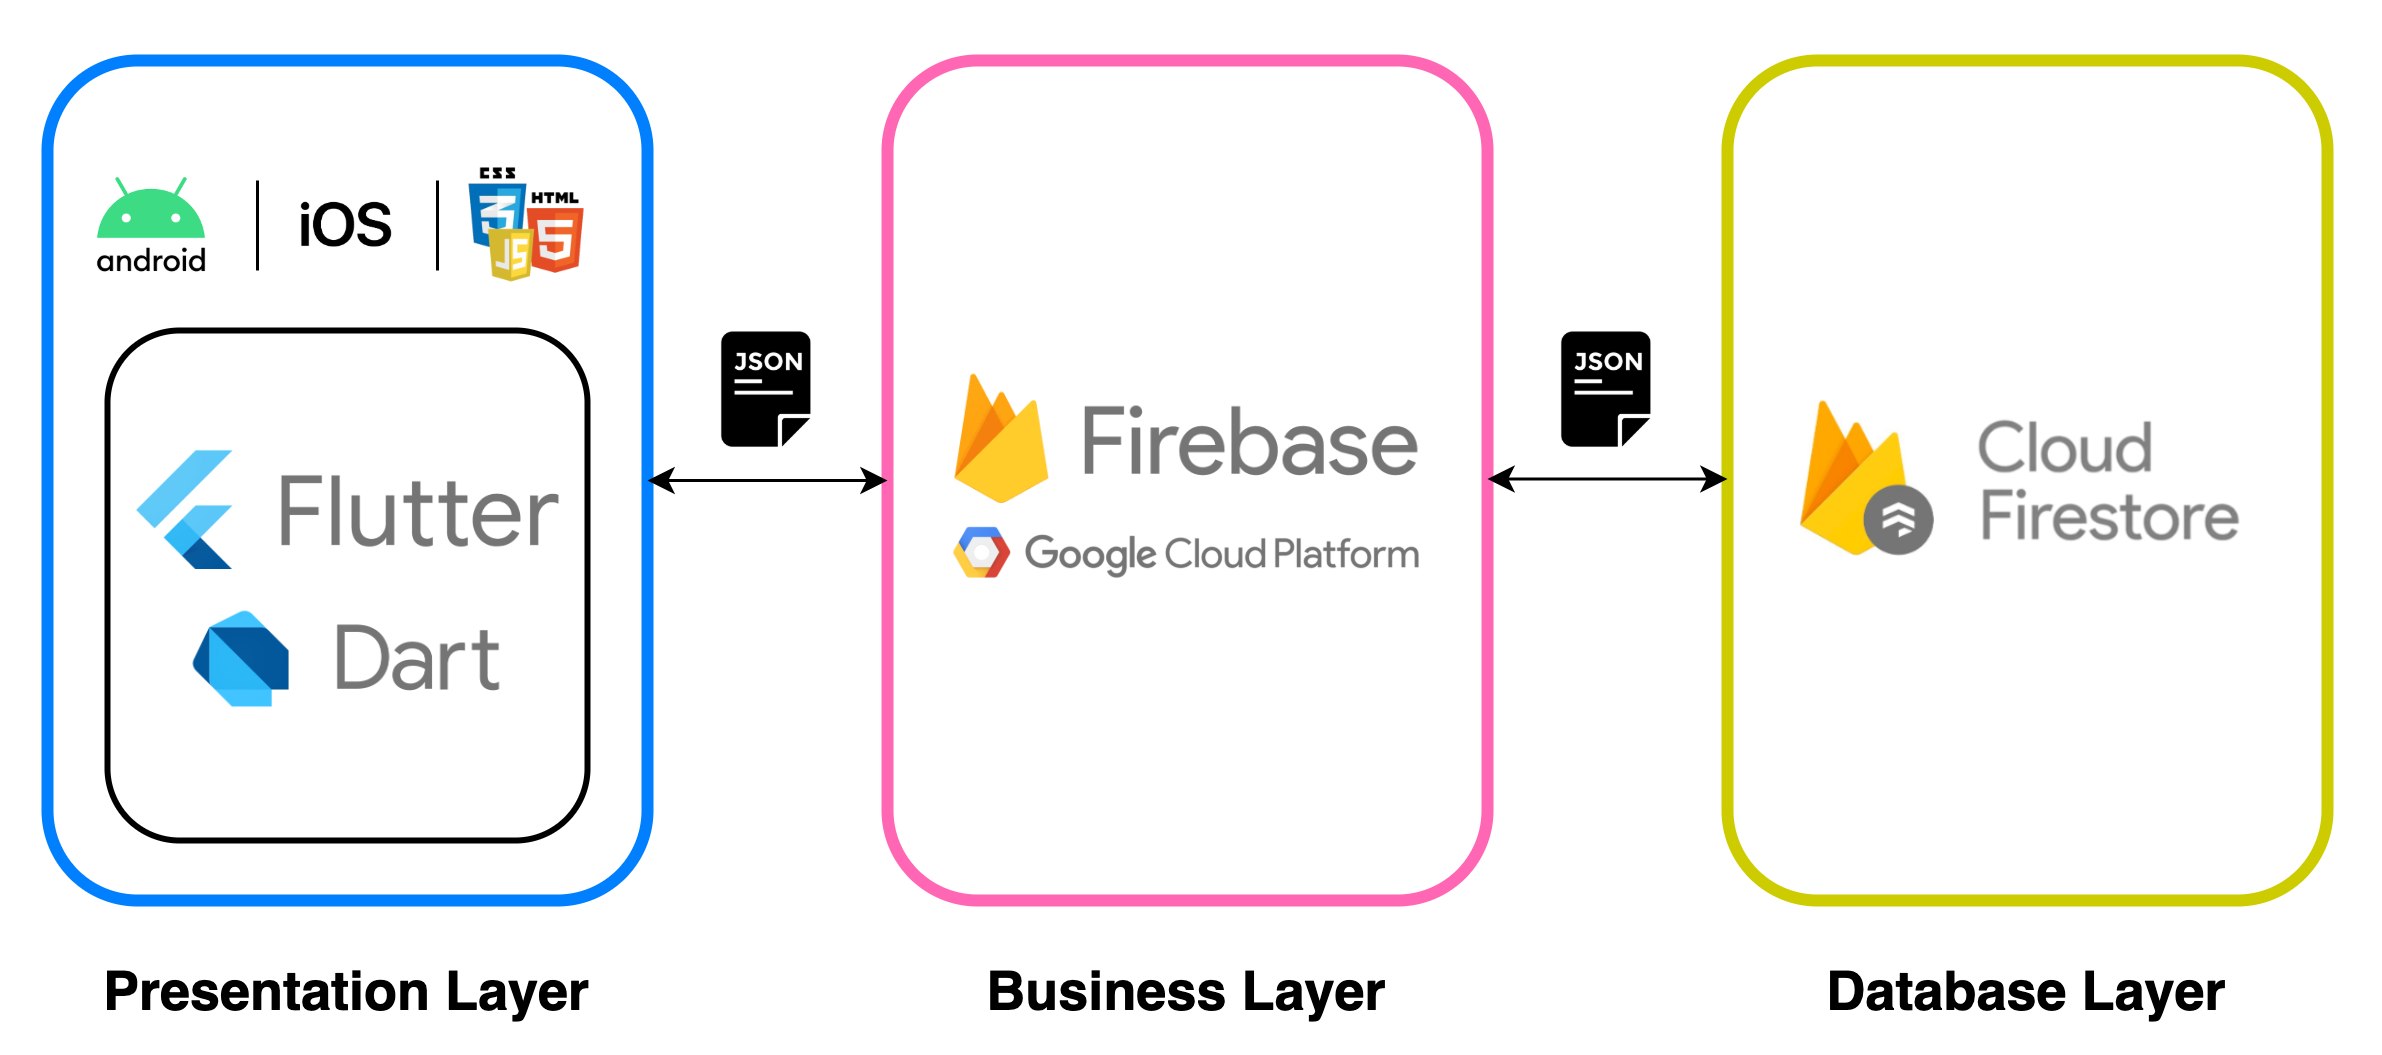
\includegraphics[width=0.8\textwidth]{./Images/arc.png}
\caption{Architecture of the Sterio system}
\label{fig:arc}
\end{figure}

\subsection{Database Layer}

The Database Layer is responsible for managing and storing all the data that it is used in the system. It receives information entered by the application's users and answers accordingly with the requested information from the Business Layer. ~\cite{Aarsten}

The first development step of the platform was the creation of an entity-relationship model so that we can model the database and determine which entities we need based on the medium-fidelity prototype described in section ~\ref{sec:userenactments}. The representation of this model, shown in Figure ~\ref{fig:eadiagram}, will help us visualize and conceptualize the system in the first stage, which will soothe the development difficulty and discard preliminary oversights.

\begin{figure}[h]
\centering
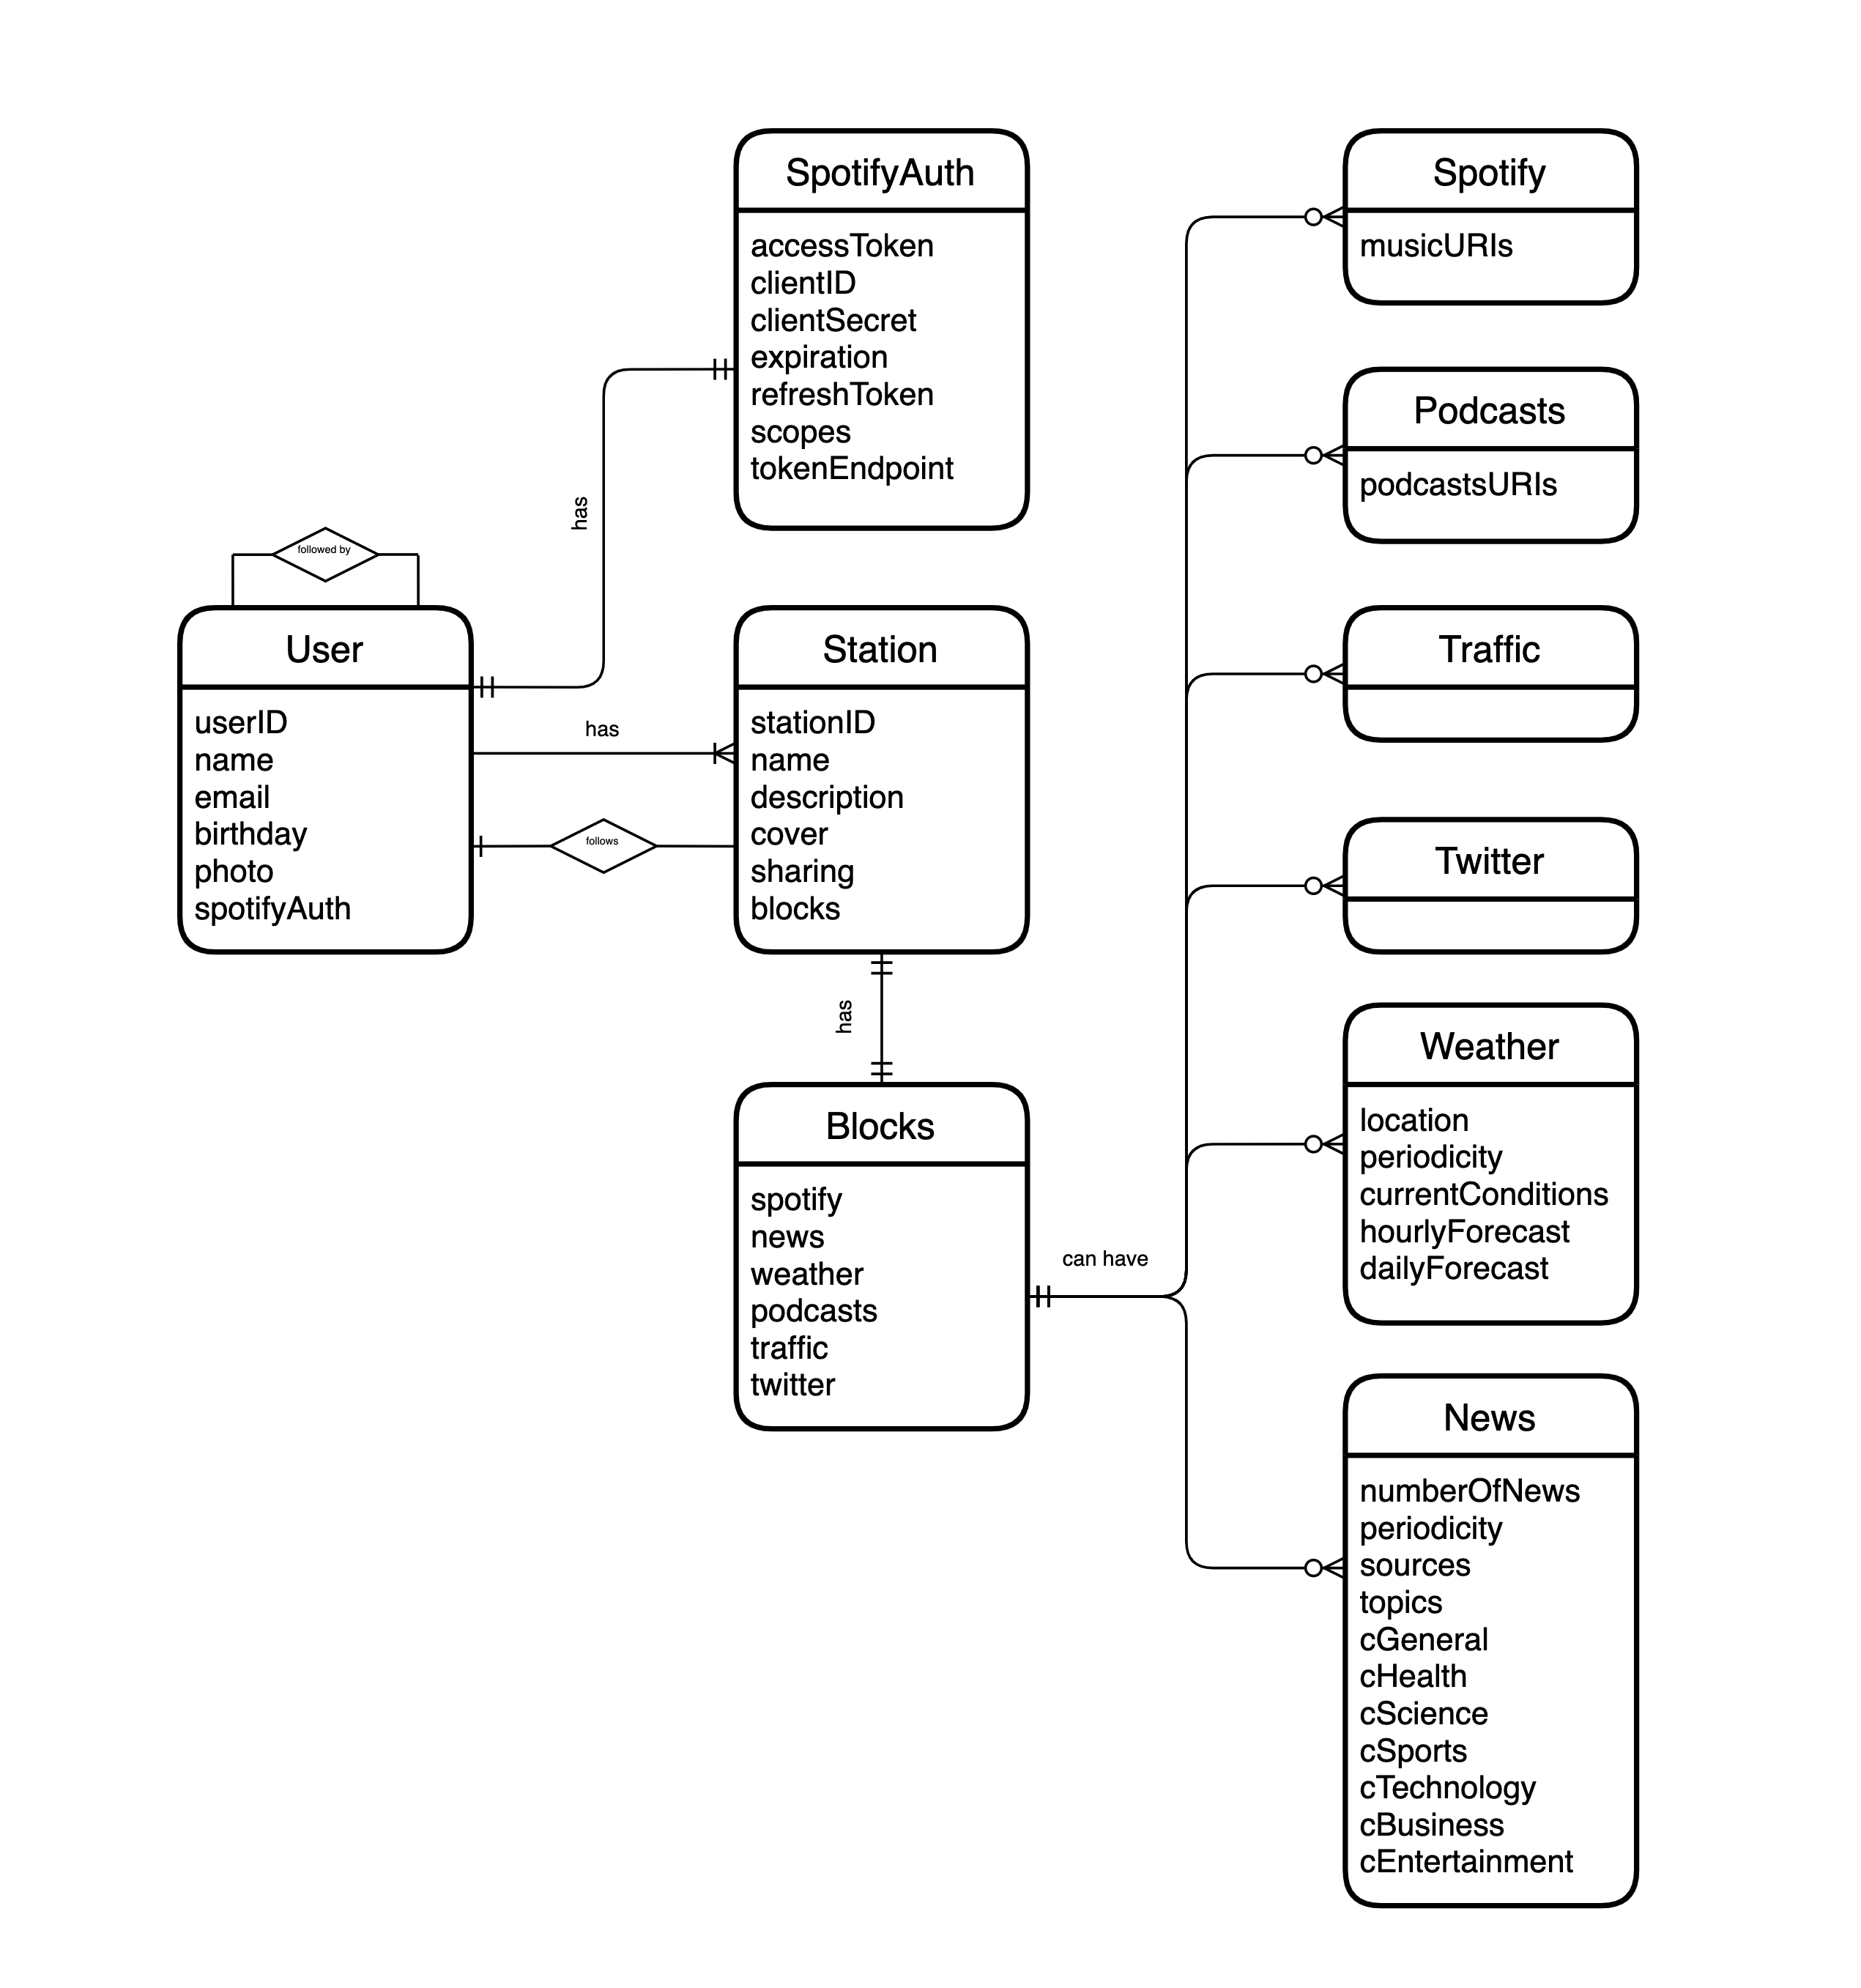
\includegraphics[width=0.8\textwidth]{./Images/ea.png}
\caption{Entity – Relationship Model of the Sterio system}
\label{fig:eadiagram}
\end{figure}


The implementation of the database was conducted using Google's Cloud Firestore~\footnote{Detailed information available on the platform's \href{https://firebase.google.com/products/firestore}{official website}.}, which is a NoSQL, document-oriented database. Being a NoSQL database, it provides several advantages, such as a non-relational and schema-less data model, low latency and high performance, highly scalable, and object-oriented programming that is easy and flexible to use. ~\cite{Stonebraker2010} Each document contains a set of key-value pairs, being optimized for storing sizable collections of small documents. It is a serverless document database that effortlessly scales to meet any demand, with no maintenance required, which accelerates the development of native cloud applications and lets developers focus their efforts on the most foreground layers of a system.

We chose to use Cloud Firestore due to its lean learning curve, ease-of-use, good performance, reliability, high scalability, and deep integration with other Google services that will also be used in the development of the platform. Furthermore, by using this technology, the system is prepared to be easily customized and to receive new data if the project has any changes in the way we approach some of its features.


\subsection{Business Layer}

The Business Layer is responsible for encoding the real-world business rules that determine how data can be created, stored, and changed. It contrasts with the remainder of the software that might be concerned with lower-level details of managing a database or displaying the user interface, system infrastructure, or generally connecting various parts of the program. ~\cite{Aarsten}

For the \textit{Sterio} platform, we chose to use Google's Firebase~\footnote{For more information on Google's Firebase and Cloud Platform services, visit its \href{https://firebase.google.com/}{official website}.} business logic features. Firebase is a \ac{MBaaS}, which is a model for providing web app and mobile app developers with a way to link their applications to backend cloud storage and \acp{API} exposed by backend applications while also providing features such as user management, push notifications, and integration with social networking services.

Firebase provides several pre-developed, robust, and reliable \acp{SDK} — such as authentication, hosting, storage, and app indexing — that helped us steer the focus of our development efforts to the design and conceiving of the user experience and interface. As with Cloud Firestore, it integrates thoroughly with other Google services — including the Google Cloud Platform, which will be used for the process and synthesizing of the text-to-speech technology — while also allowing the configuration of third-party \acp{API} that will be used in the context of our project.

\subsection{Presentation Layer}

The third and final layer of the system is the Presentation Layer, which is responsible for the interaction between the user and the system. ~\cite{Aarsten} This layer will interact with the business layer through calls to the Firebase service.

Based on the preliminary user research presented in Section ~\ref{chap:userresearch}, and corroborating with the data shown in Figure ~\ref{chart:devices}, most users listen to music streaming services on their smartphone. Furthermore, as we want our platform to be easily accessible on the go, we focused our efforts on analyzing the most popular mobile development frameworks to develop our platform on.

\begin{figure}
	\centering
	\caption{Share of internet users who have used a music streaming services in the last month worldwide in 2nd quarter 2017, by device (Statista / GlobalWebIndex)}
	\label{chart:devices}
	\begin{bchart}[step=10,max=45,unit=\%,width=0.8\textwidth]
        \bcbar[text=Smartphone (Mobile)]{39}
            \smallskip
        \bcbar[text=PC / Laptop]{30}
            \smallskip
        \bcbar[text=Tablet]{8}
    \end{bchart}
\end{figure}


We chose to develop the Sterio platform using Flutter~\footnote{To learn more about the Flutter framework, consult the \href{https://flutter.dev/}{official website}.}, which is an \ac{UI} toolkit for building natively compiled applications for mobile, web, and desktop from a single codebase. Flutter apps are written in the Dart~\footnote{For more information on the Dart programming language, visit its \href{https://dart.dev/}{official website}.} programming language and make use of many of the language's more advanced features. ~\cite{Payne2019}

In the context of our project, Flutter has some key advantages over other technologies. To start, although it has been built as a mobile-first toolkit in the first stage, Flutter is now a cross-platform development tool that allows the development of mobile (on the Android and iOS operating systems) and desktop apps without compounding changes to the codebase. This ensures that our platform renders well on a variety of devices and windows or screen sizes, without limiting our endeavors. ~\cite{H.GillbertMiller2011} Secondly, in comparison with other mobile frameworks, Flutter reduces the code development time by a wide margin. In a large and complex project such as ours, this is a crucial advantage that will lead us to a robust final product without the need for allocating umpteen resources. Finally, Flutter offers a variety of advanced tools that allow us to achieve a great user experience and interface design, which will help us achieve our goals. ~\cite{Payne2019}

% #############################################################################

\section{Functional Prototype}

Based on the medium-fidelity prototype presented in Section ~\ref{sec:userenactments}, the last — and most crucial — step of the development cycle was to construct a functional prototype with a fully-working set of features. This prototype should resemble as close as possible to the final representation of the system. 

In the following subsections, we describe in detail all functionalities, components, screens, implementations, and technical facets of the \textit{Sterio} system, as well as the design implications and limitations faced during the development of the prototype. We begin by examining the four main screens of the application — 'Home', 'Search', 'Social', and 'My Stations' — followed by an analysis of the technical reasoning behind our development rulings.

\newpage
\subsection{Login, Signup, and Authentication}
\label{subsec:lsa}

The first interaction the user has with the \textit{Sterio} platform is the login/signup screen, shown in Figure ~\ref{fig:login1}. There, the user can choose to login with an Apple or Facebook account, or with an e-mail. If the user chooses to use one of the first two methods, an in-app browser window is shown so that the user can enter the required credentials. If the user chooses to use an e-mail as a signup method, the screen is shown in ~\ref{fig:login2} is presented.

\begin{figure}[htbp]
	\centering
	\subfigure[Login / Signup screen]{\label{fig:login1}
	\frame{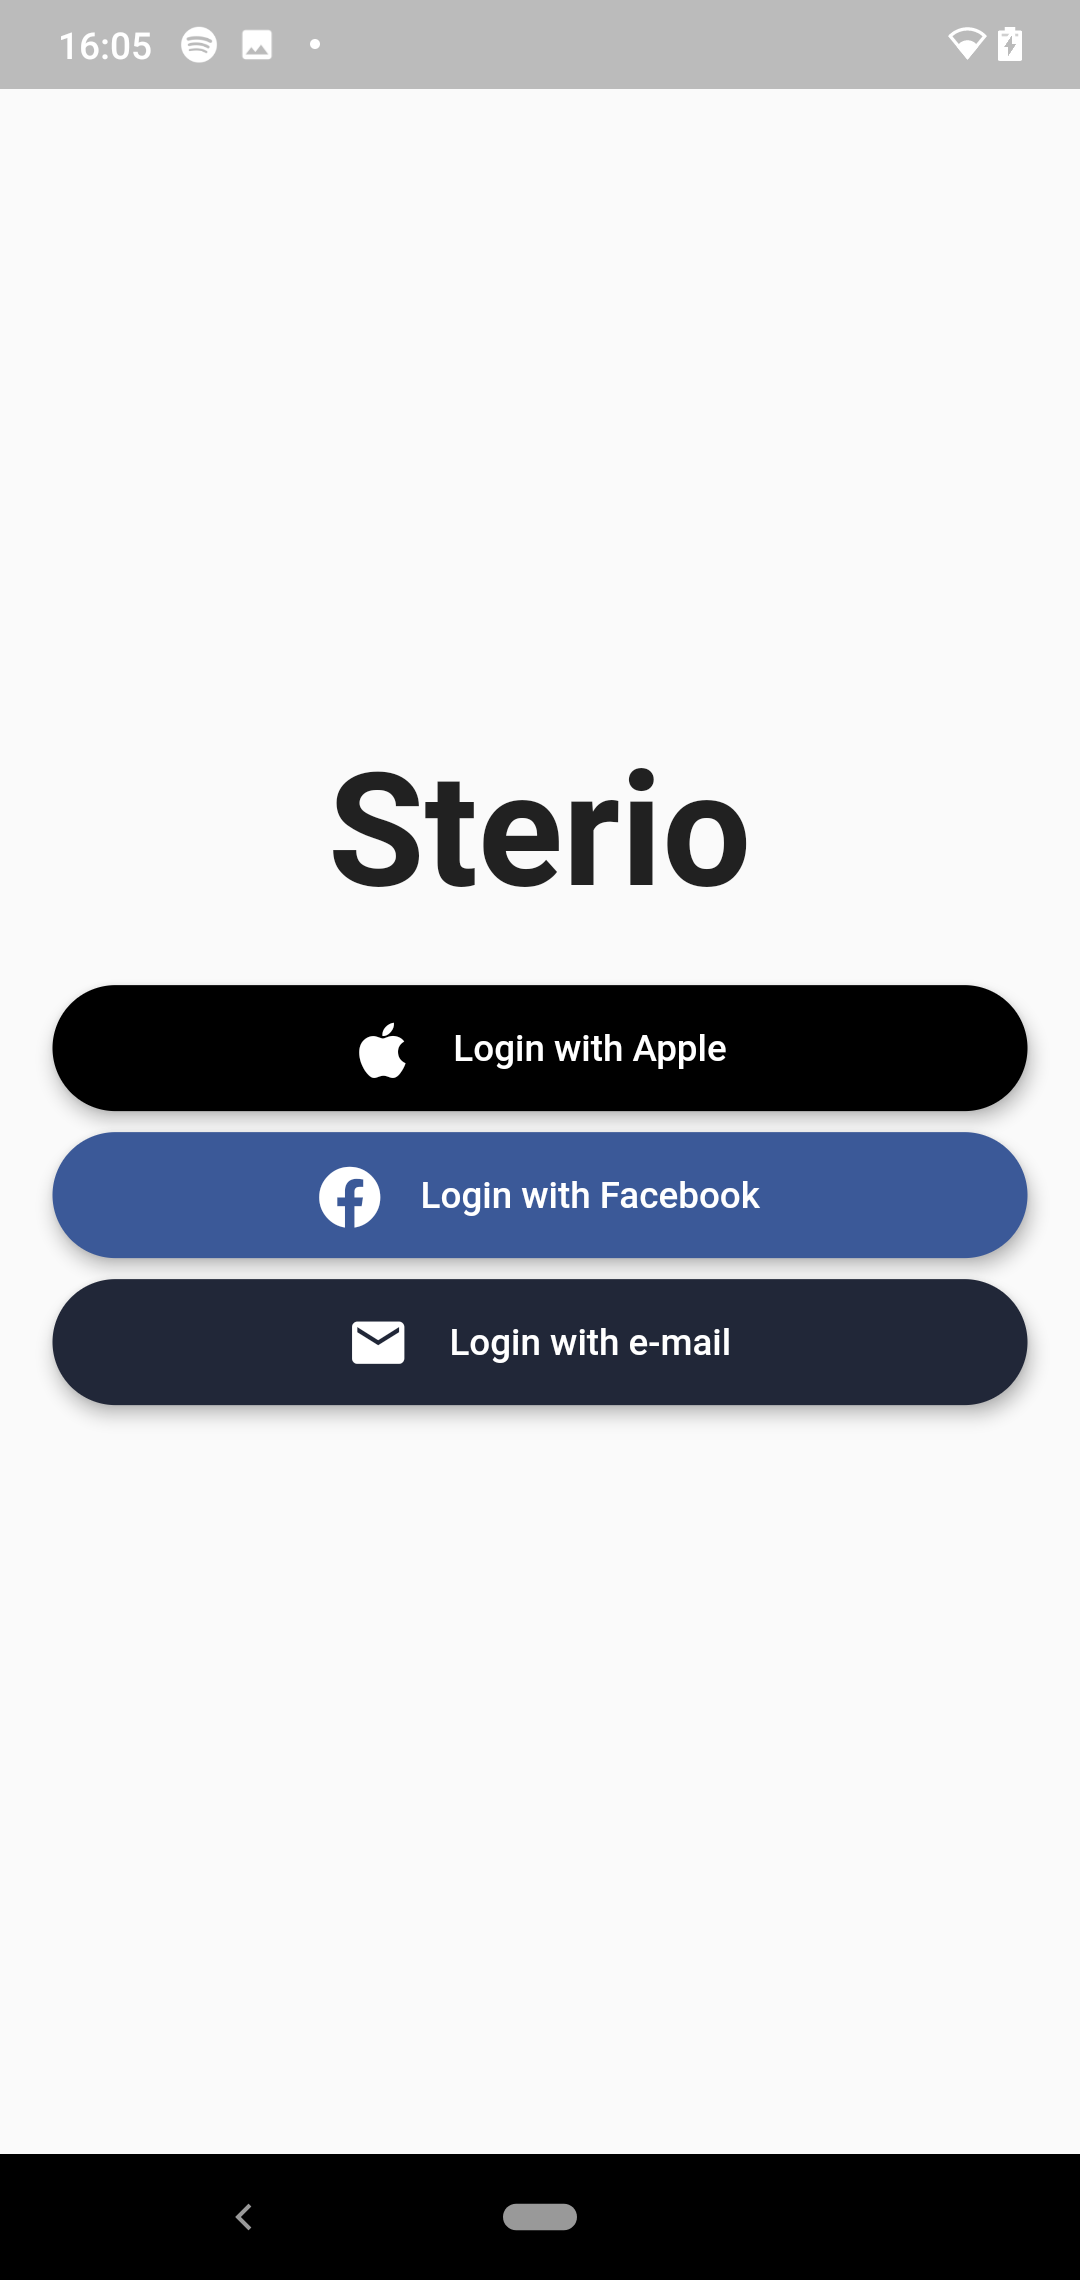
\includegraphics[width=0.29\textwidth]{./Images/screenshots/login1.png}}} \qquad
	\subfigure[Login with e-mail]{\label{fig:login2}
	\frame{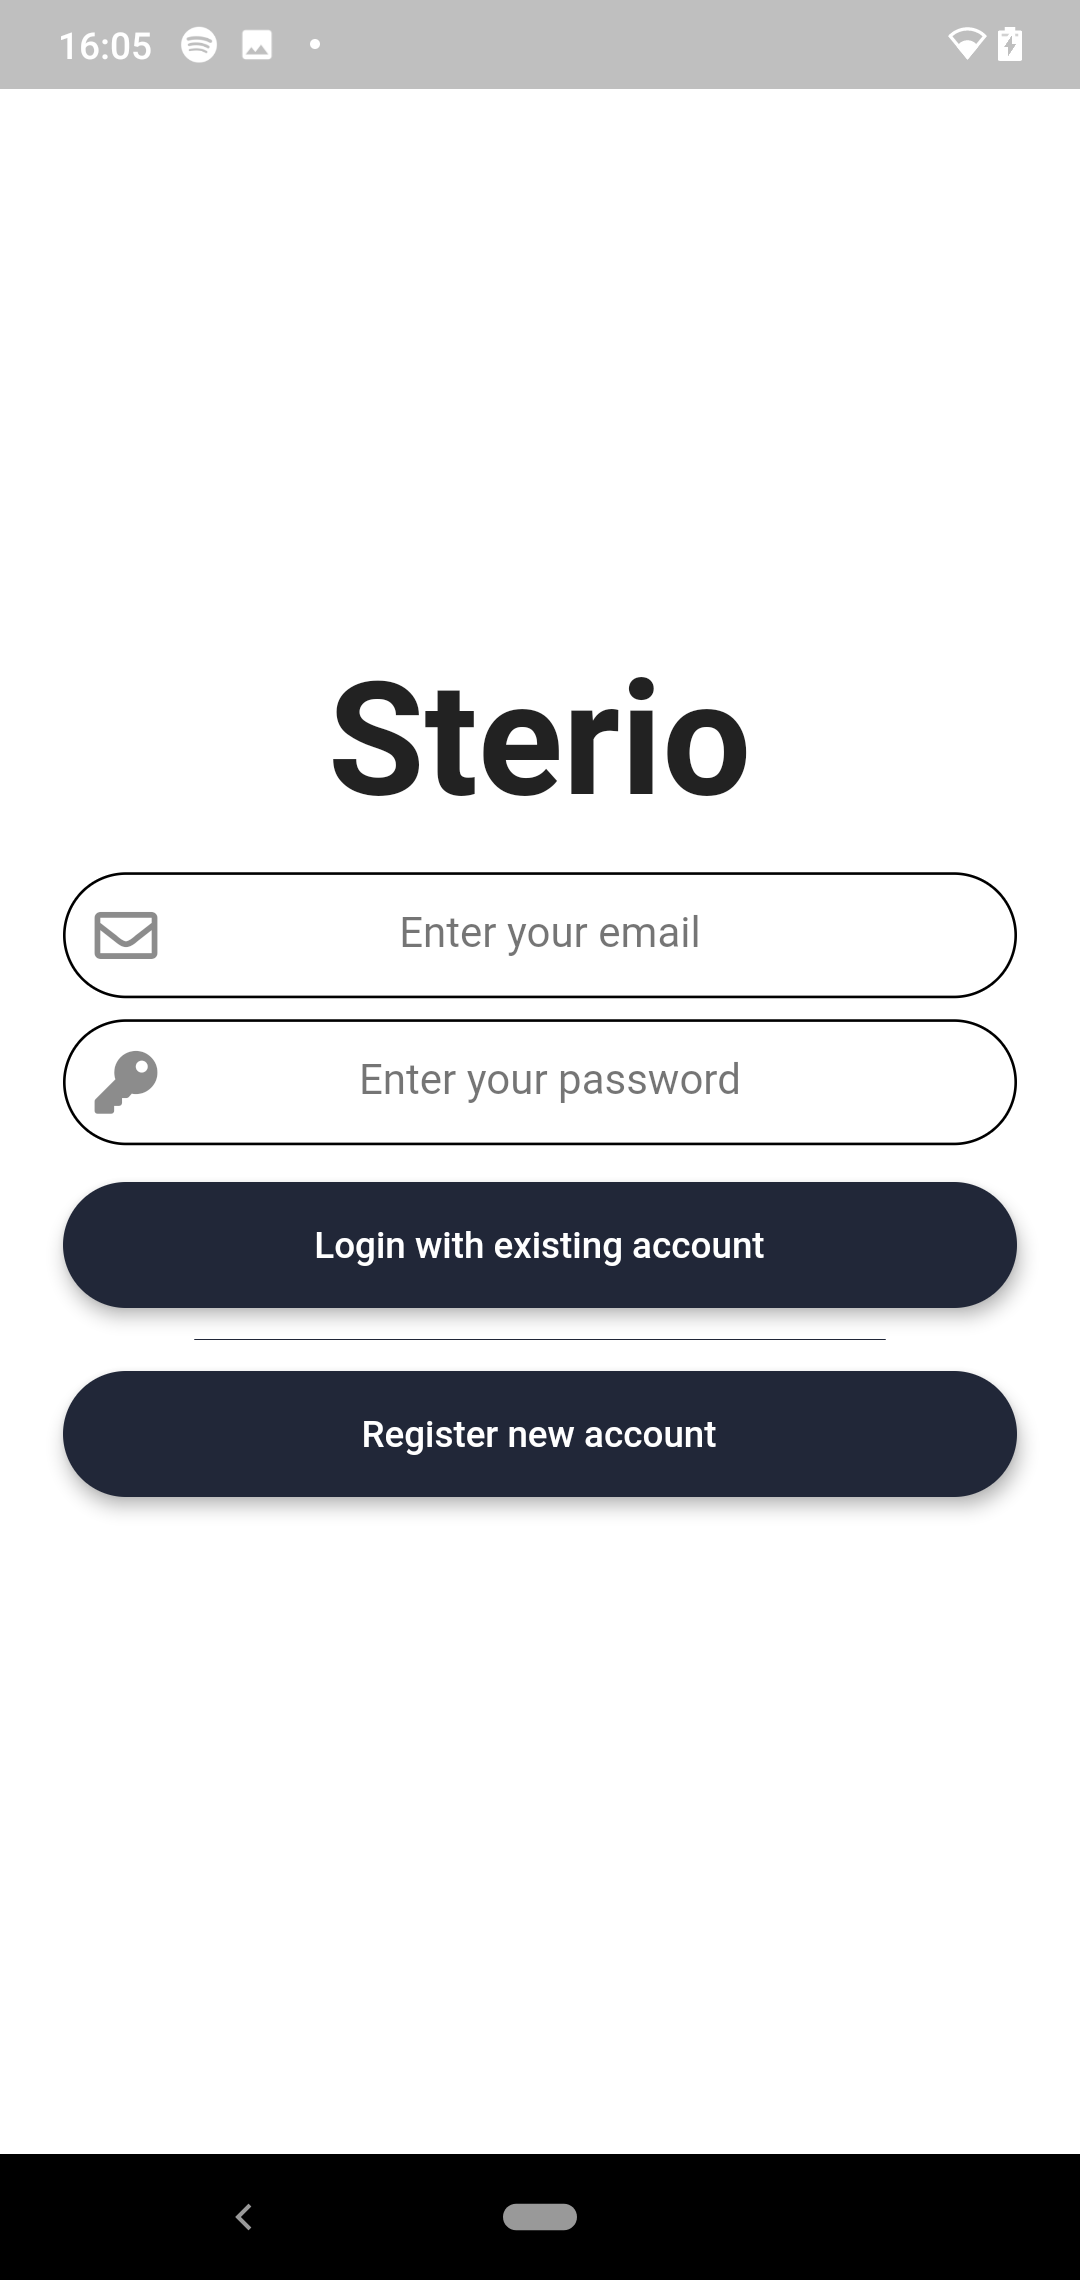
\includegraphics[width=0.29\textwidth]{./Images/screenshots/login2.png}}} \qquad
	\subfigure[Spotify authentication]{\label{fig:auth}
	\frame{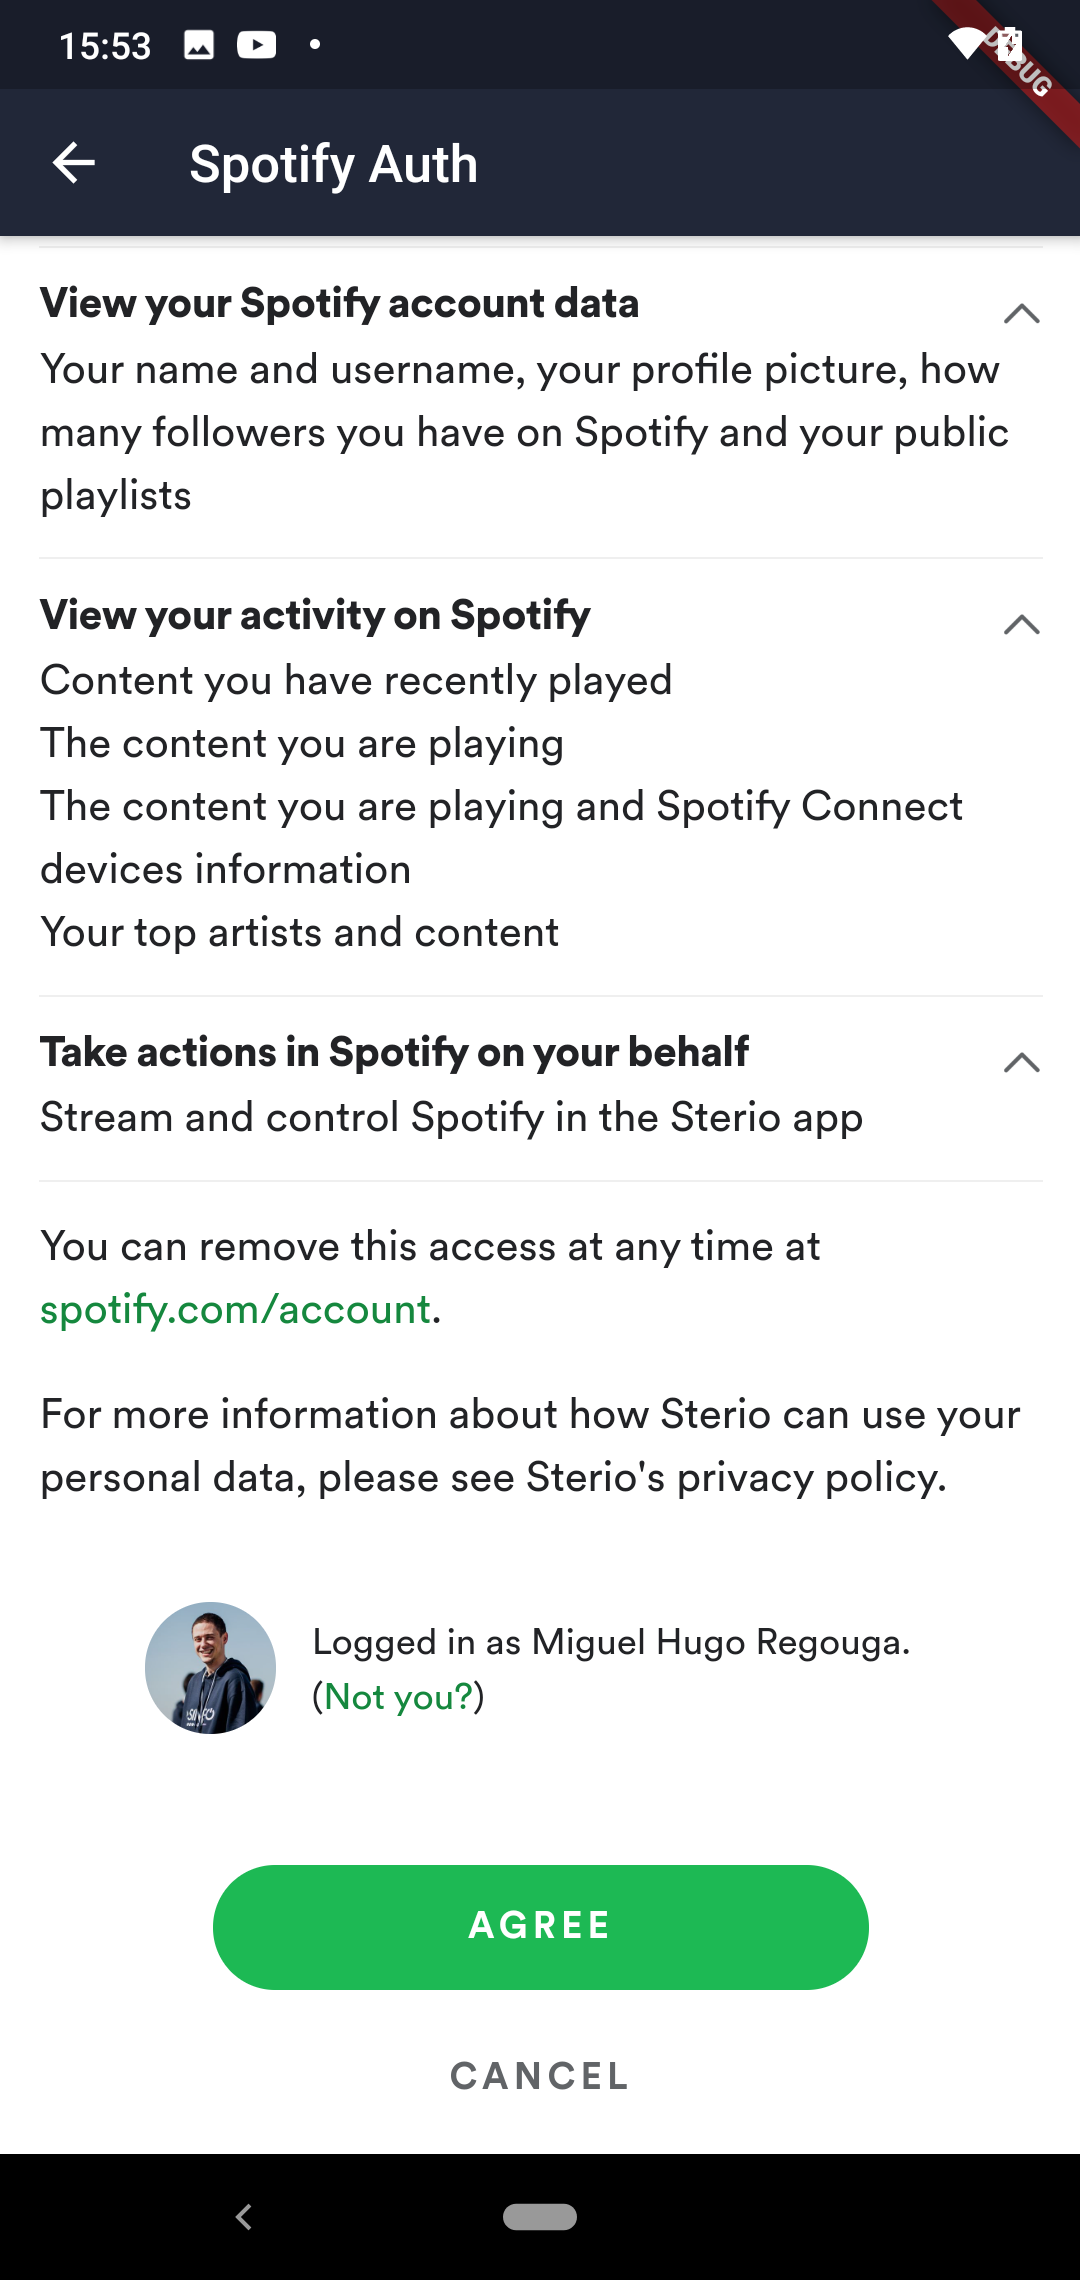
\includegraphics[width=0.29\textwidth]{./Images/screenshots/auth.png}}} \qquad
	\caption{Login, Signup, and Spotify authentication screens}
	\label{fig:lss}
\end{figure}

As the system integrates with a Spotify Premium account, it is also necessary that the user authenticates with the music streaming service, so that we can take advantage of its ~\ac{API}. To do so, an in-app browser window, shown in Figure ~\ref{fig:auth}, is also presented to the user. This is a one-time step, as the system stores the necessary ~\ac{API} parameters in the database and automatically logs in the user in future usages.

\newpage
\subsection{'Home' and 'Search' Screens}
\begin{figure}[htbp]
	\centering
	\subfigure['Home' screen]{\label{fig:homes}
	\frame{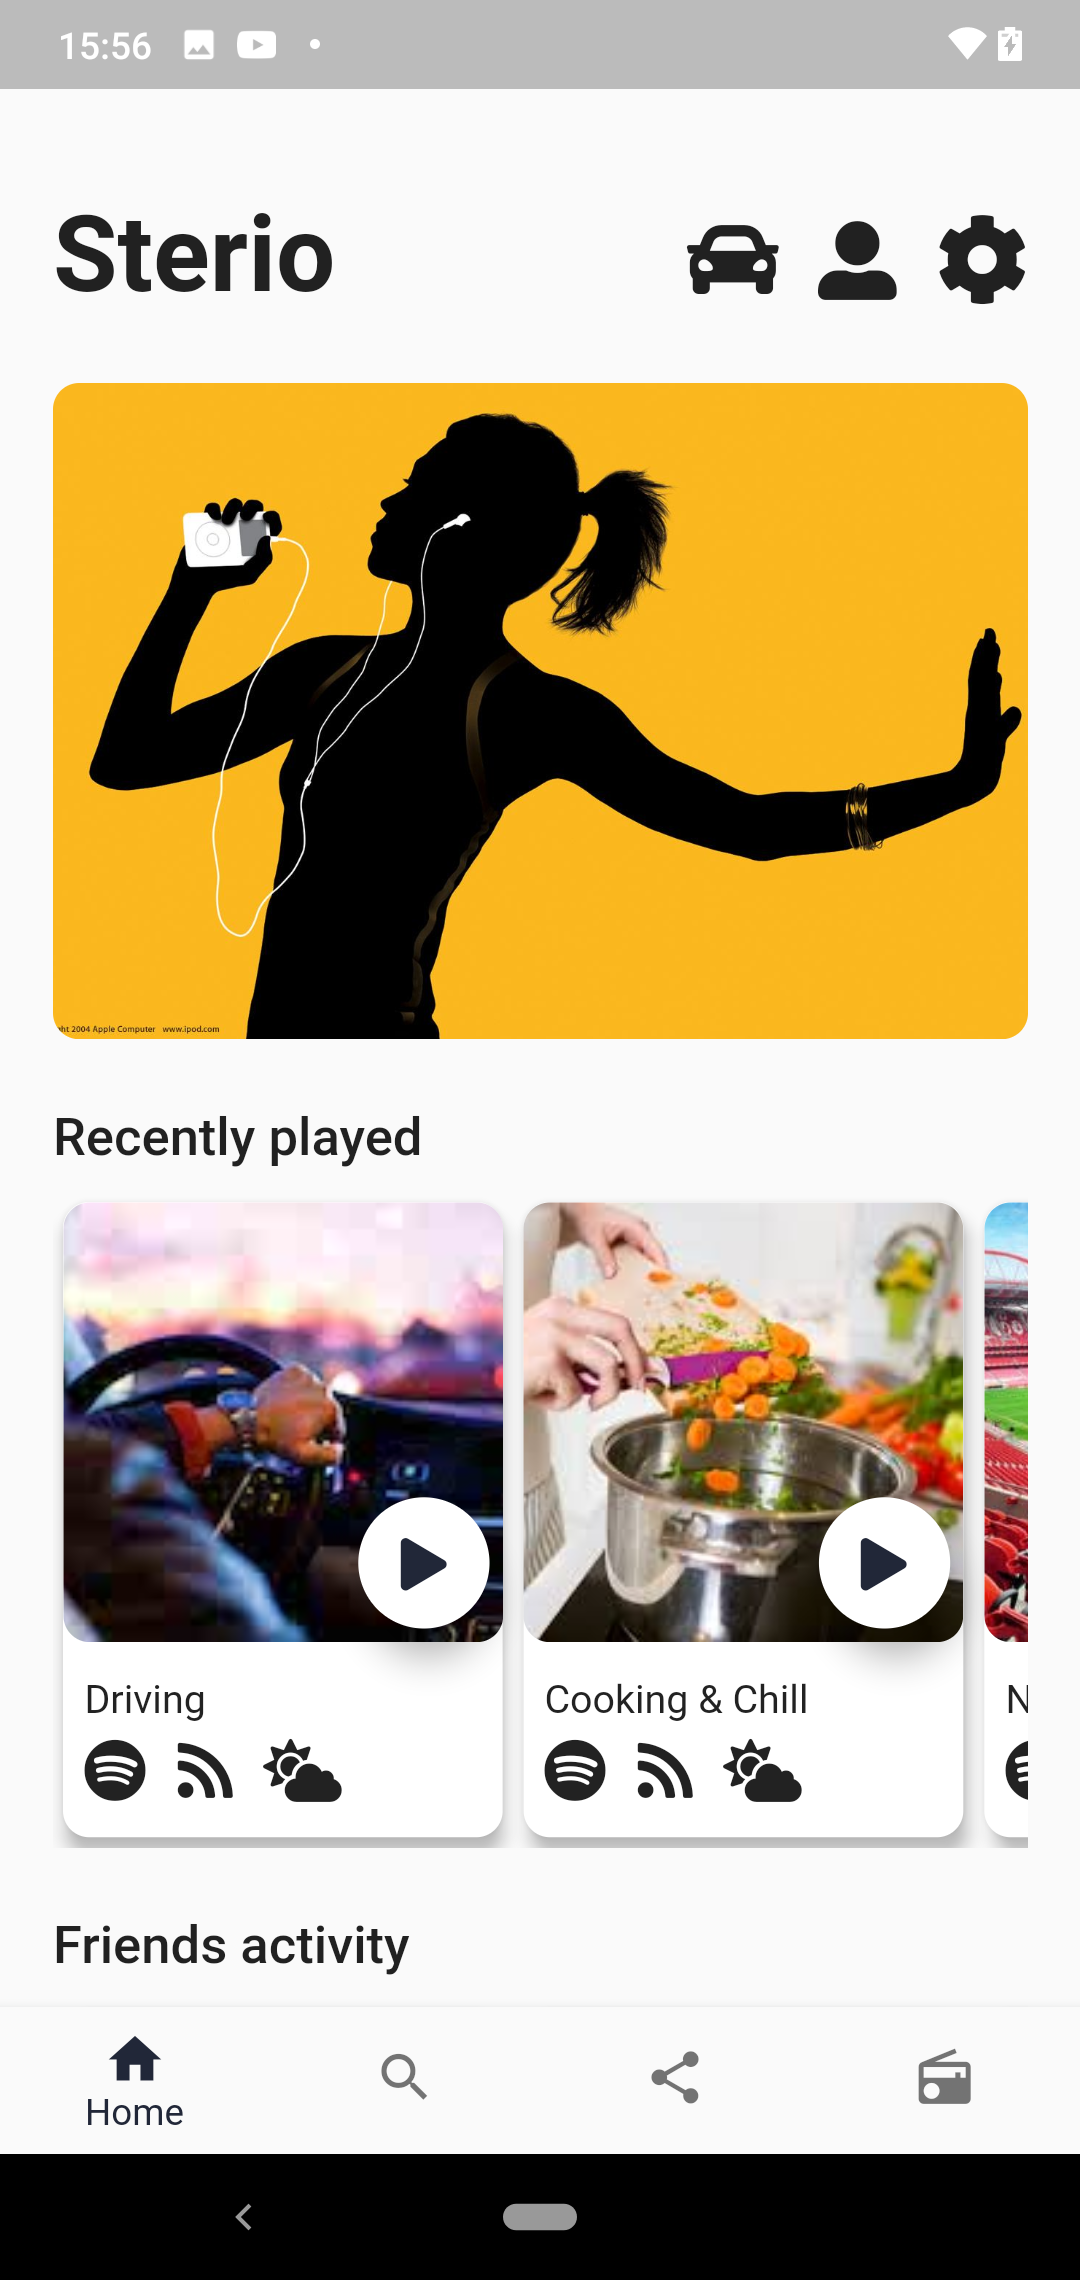
\includegraphics[width=0.29\textwidth]{./Images/screenshots/home.png}}} \qquad
	\subfigure['Search' screen]{\label{fig:searchs1}
	\frame{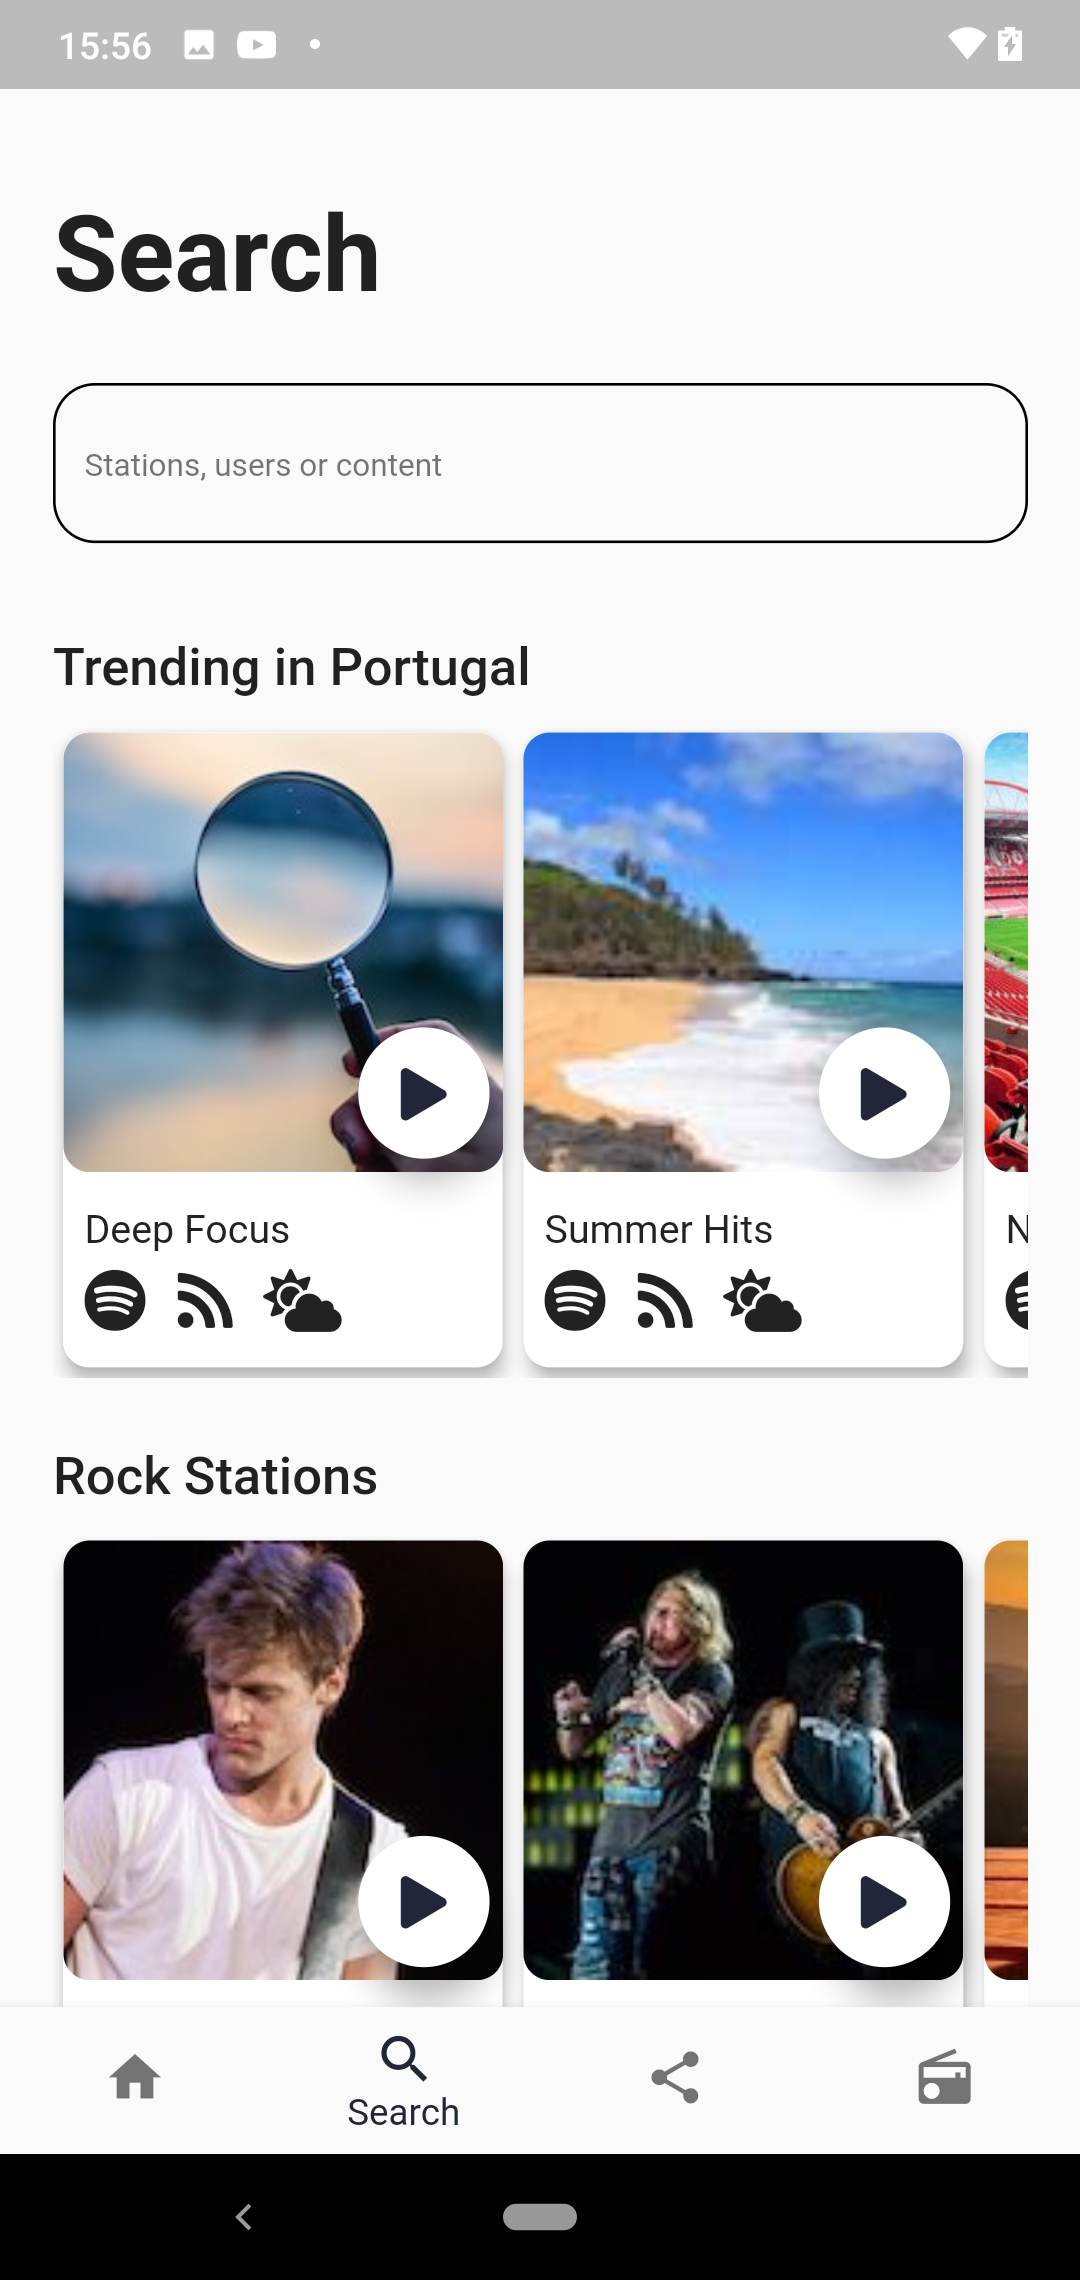
\includegraphics[width=0.29\textwidth]{./Images/screenshots/search.png}}} \qquad
	\caption{'Home' and 'Search' screens}
	\label{fig:mfp1}
\end{figure}

After logging in, the user is prompted with the 'Home' screen, shown in Figure ~\ref{fig:homes}, which is the first and most foregrounding screen of the platform. In this screen, the user can quickly play a station based on recent activity, friends activity, top charts, or other relevant information tailored to the user's taste and usability history. In this screen, the user can also change the settings and preferences of the app, as well as of the signed-in account. Finally, the user can also enter the "Car Mode" of the system, which transforms the ~\ac{UI} in a stripped-down, non-distracting, and easy way for the user to control playback while driving.

In the 'Search' screen, shown in Figure ~\ref{fig:searchs1}, the user can search for a specific station, content, or even other users to follow and check their profiles. In the same screen, listening suggestions are also shown, based on the most searched items and trending stations in a given location.

\newpage
\subsection{'Social' Screen}

The 'Social' screen aggregates all the social activity of the profiles that a given user follows. From there, users can explore what stations their followers are currently listening to, as well as to listen along to such stations (mimicking the experience of a traditional terrestrial radio station). 
\begin{figure}[htbp]
	\centering
	\subfigure[Social screen showing friends that are playing a station]{\label{fig:social1}
	\frame{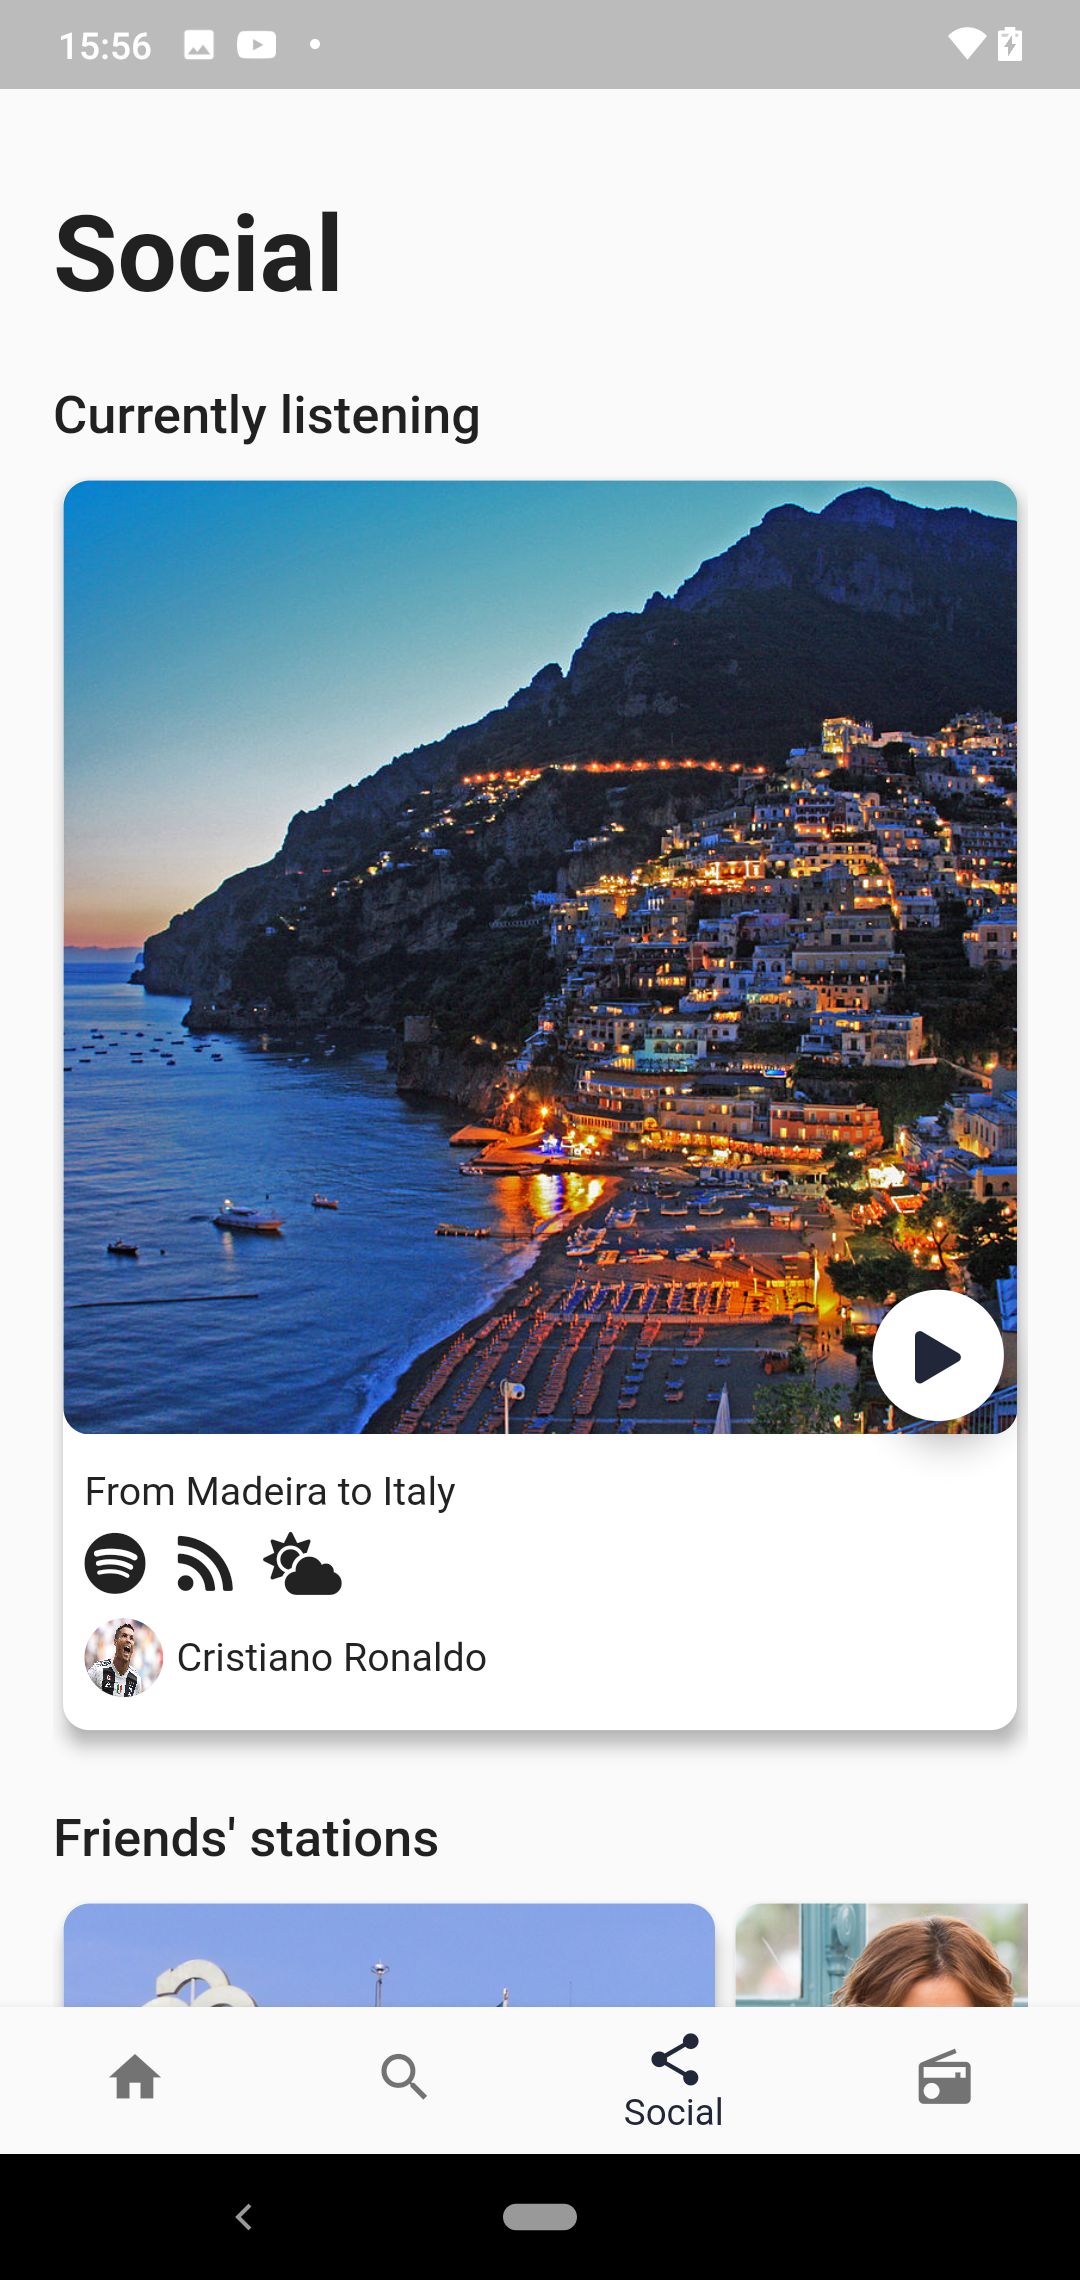
\includegraphics[width=0.29\textwidth]{./Images/screenshots/social1.png}}} \qquad
	\subfigure[Social screen with following suggestions]{\label{fig:social2}
	\frame{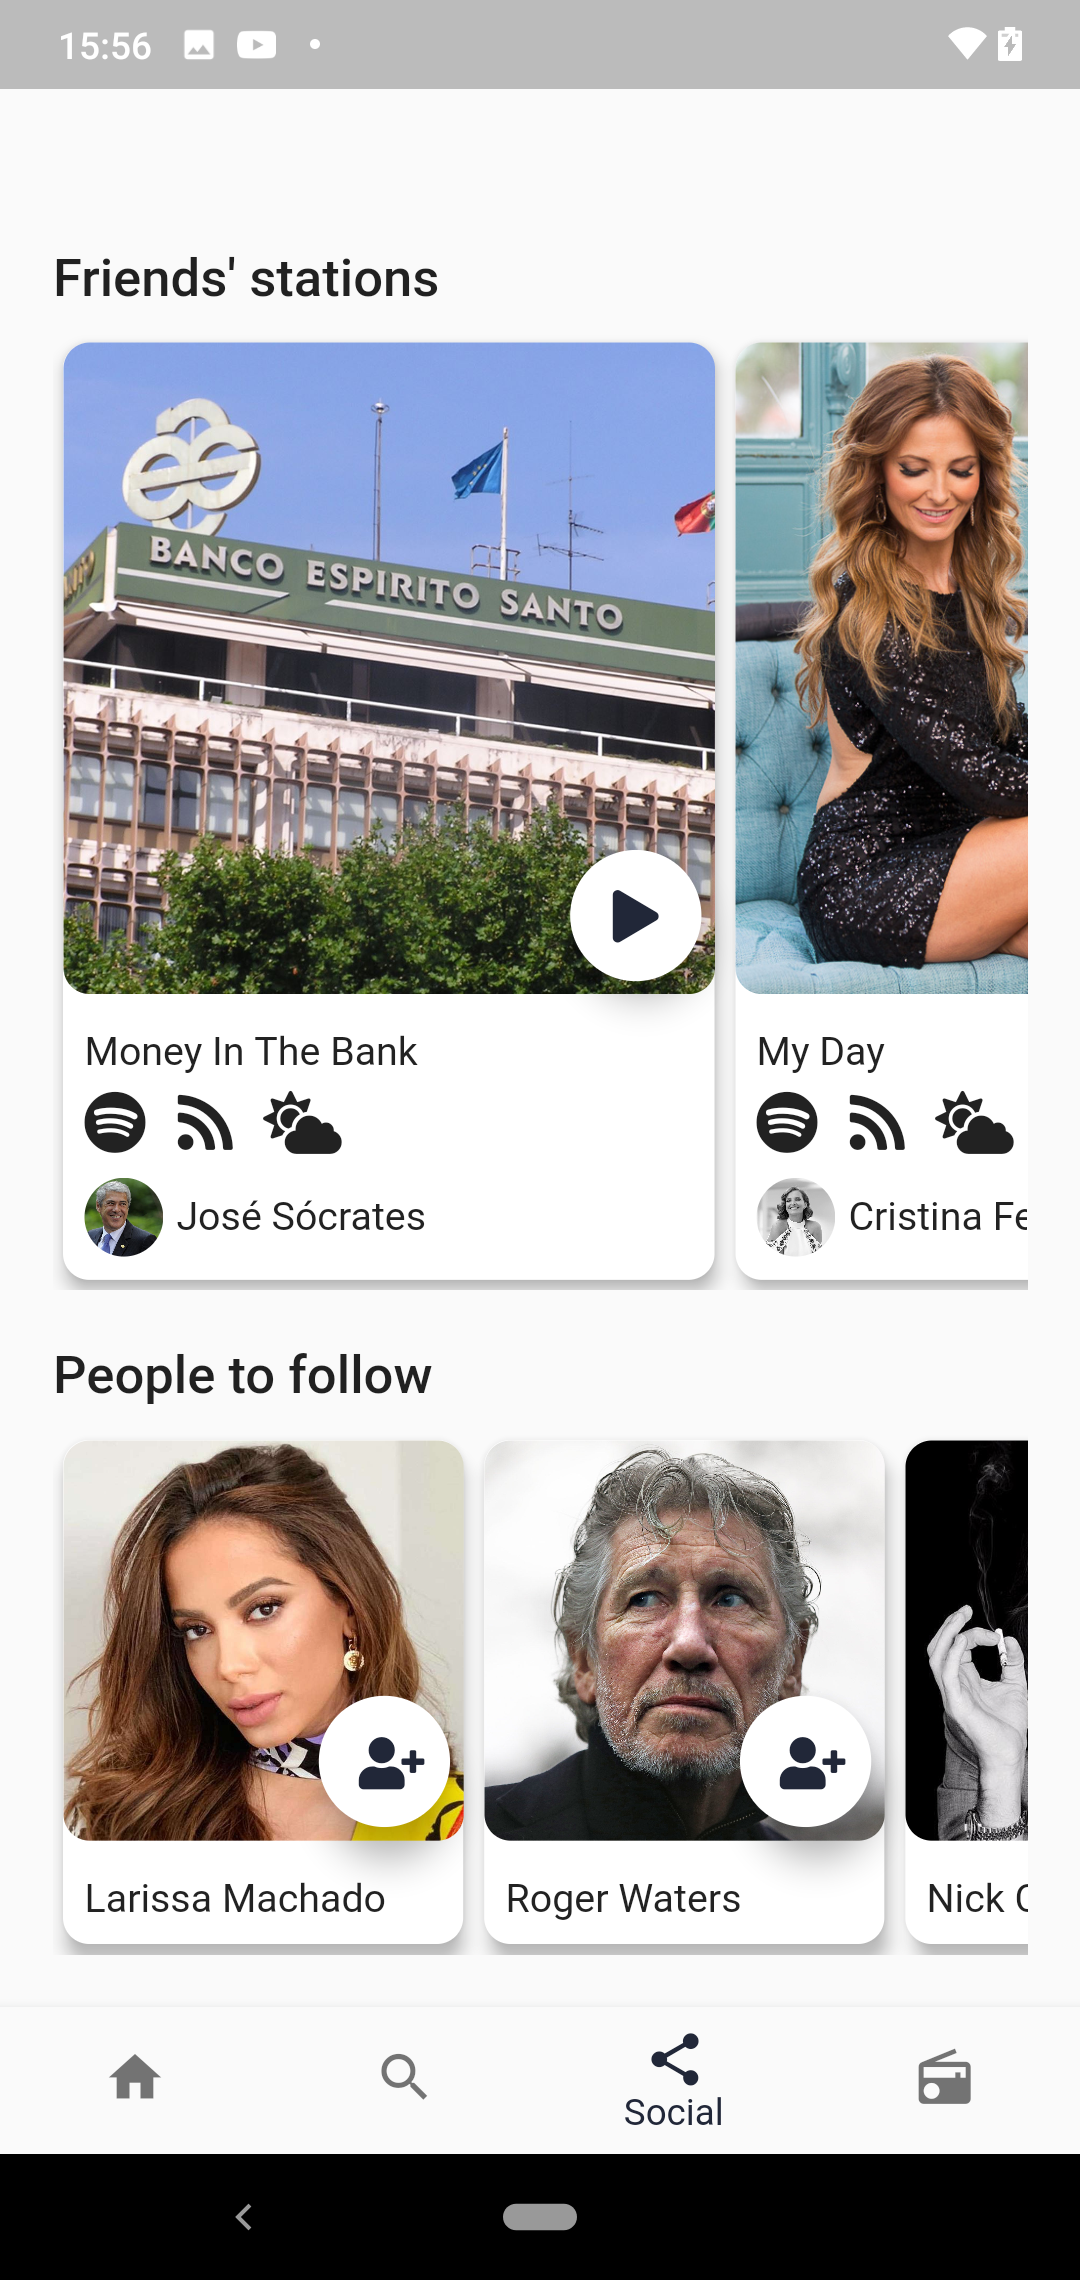
\includegraphics[width=0.29\textwidth]{./Images/screenshots/social2.png}}} \qquad
	\caption{'Social' screen}
	\label{fig:mfp1}
\end{figure}

From the same screen, users can also delve into the shared stations of their friends and family and get recommendations of profiles to follow based on their taste and friends' circle. Coinciding with a news feed of a traditional social network, users can also share and interact with shared media posts, creating a very integrated and cohesive social experience among the users of the platform.

\newpage
\subsection{'My Stations' Screen}

The last of the four main screens of the platform is the 'My Stations' screen, shown in Figure ~\ref{fig:mys}, where the user can find their own created stations, or saved stations created by other users of the platform. It acts as a 'library' of saved stations, making it easy for users to find their desired content. On the same screen, users can press the '+' red button and start the process of creating a new station, which will be added automatically to their library.

\begin{figure}[h]
\centering
\frame{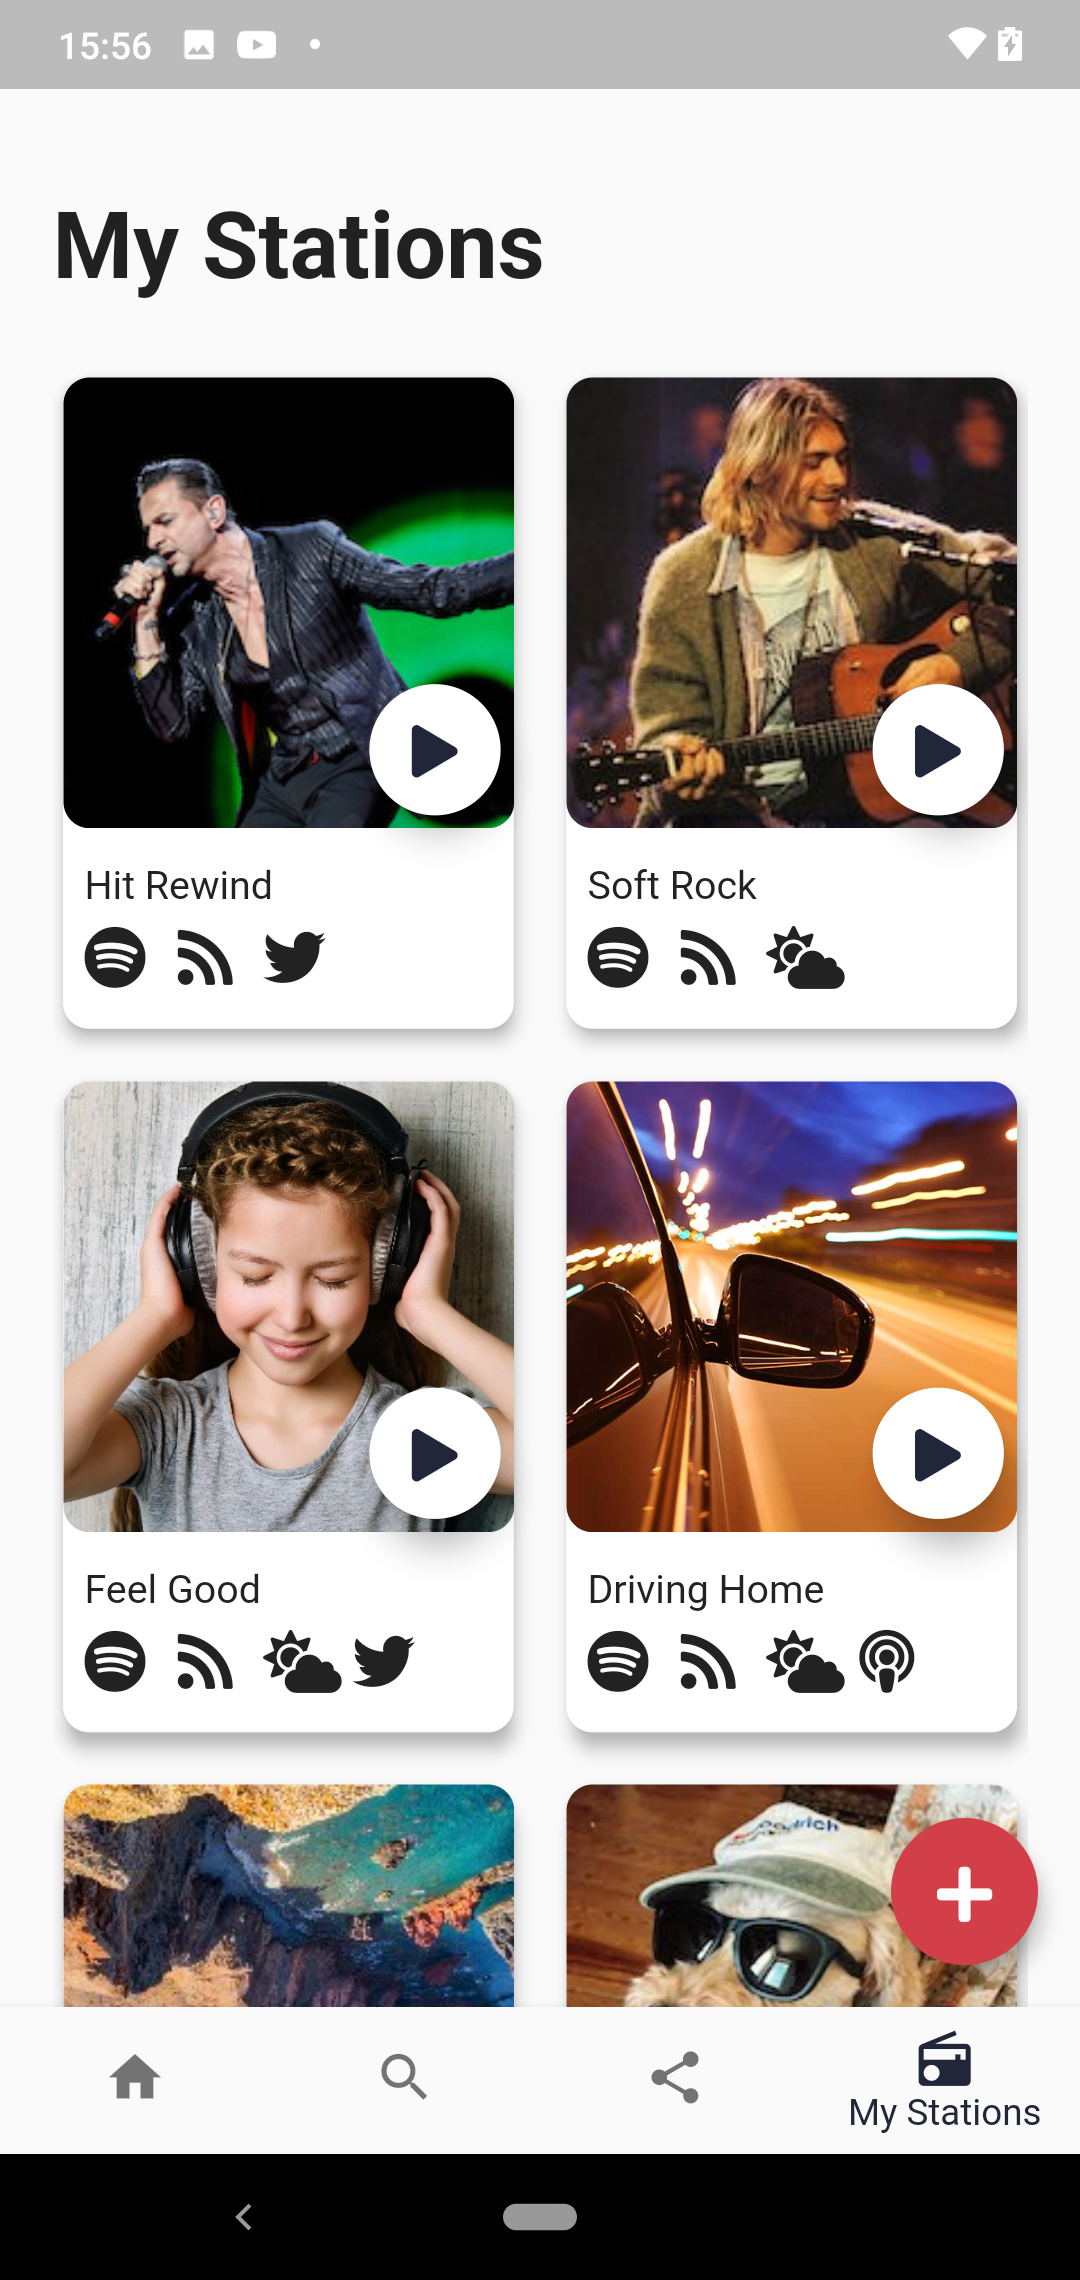
\includegraphics[width=0.29\textwidth]{./Images/screenshots/mys.png}}
\caption{'My Stations' screen}
\label{fig:mys}
\end{figure}

Each station is represented by a 'card' that displays its basic information — name, blocks, and artwork/cover. This configuration allows the user to have a glimpse of what are the contents of a given station without even entering the station's page. Furthermore, a convenient 'play' button is exposed so that users can effortlessly start playing a given station. This design is carried out across the platform's screens, creating a broad, cohesive, and consistent user experience.

All the station information is stored and loaded from the database on-demand, thus minimizing cache and offline efforts. Nevertheless, in case the user doesn't have a connection to the internet, it is possible to download and locally store a given station.


\newpage
\subsection{Creating a New Station}

\begin{figure}[htbp]
	\centering
	\subfigure[Step 1 (stations' details)]{\label{fig:ns1}
	\frame{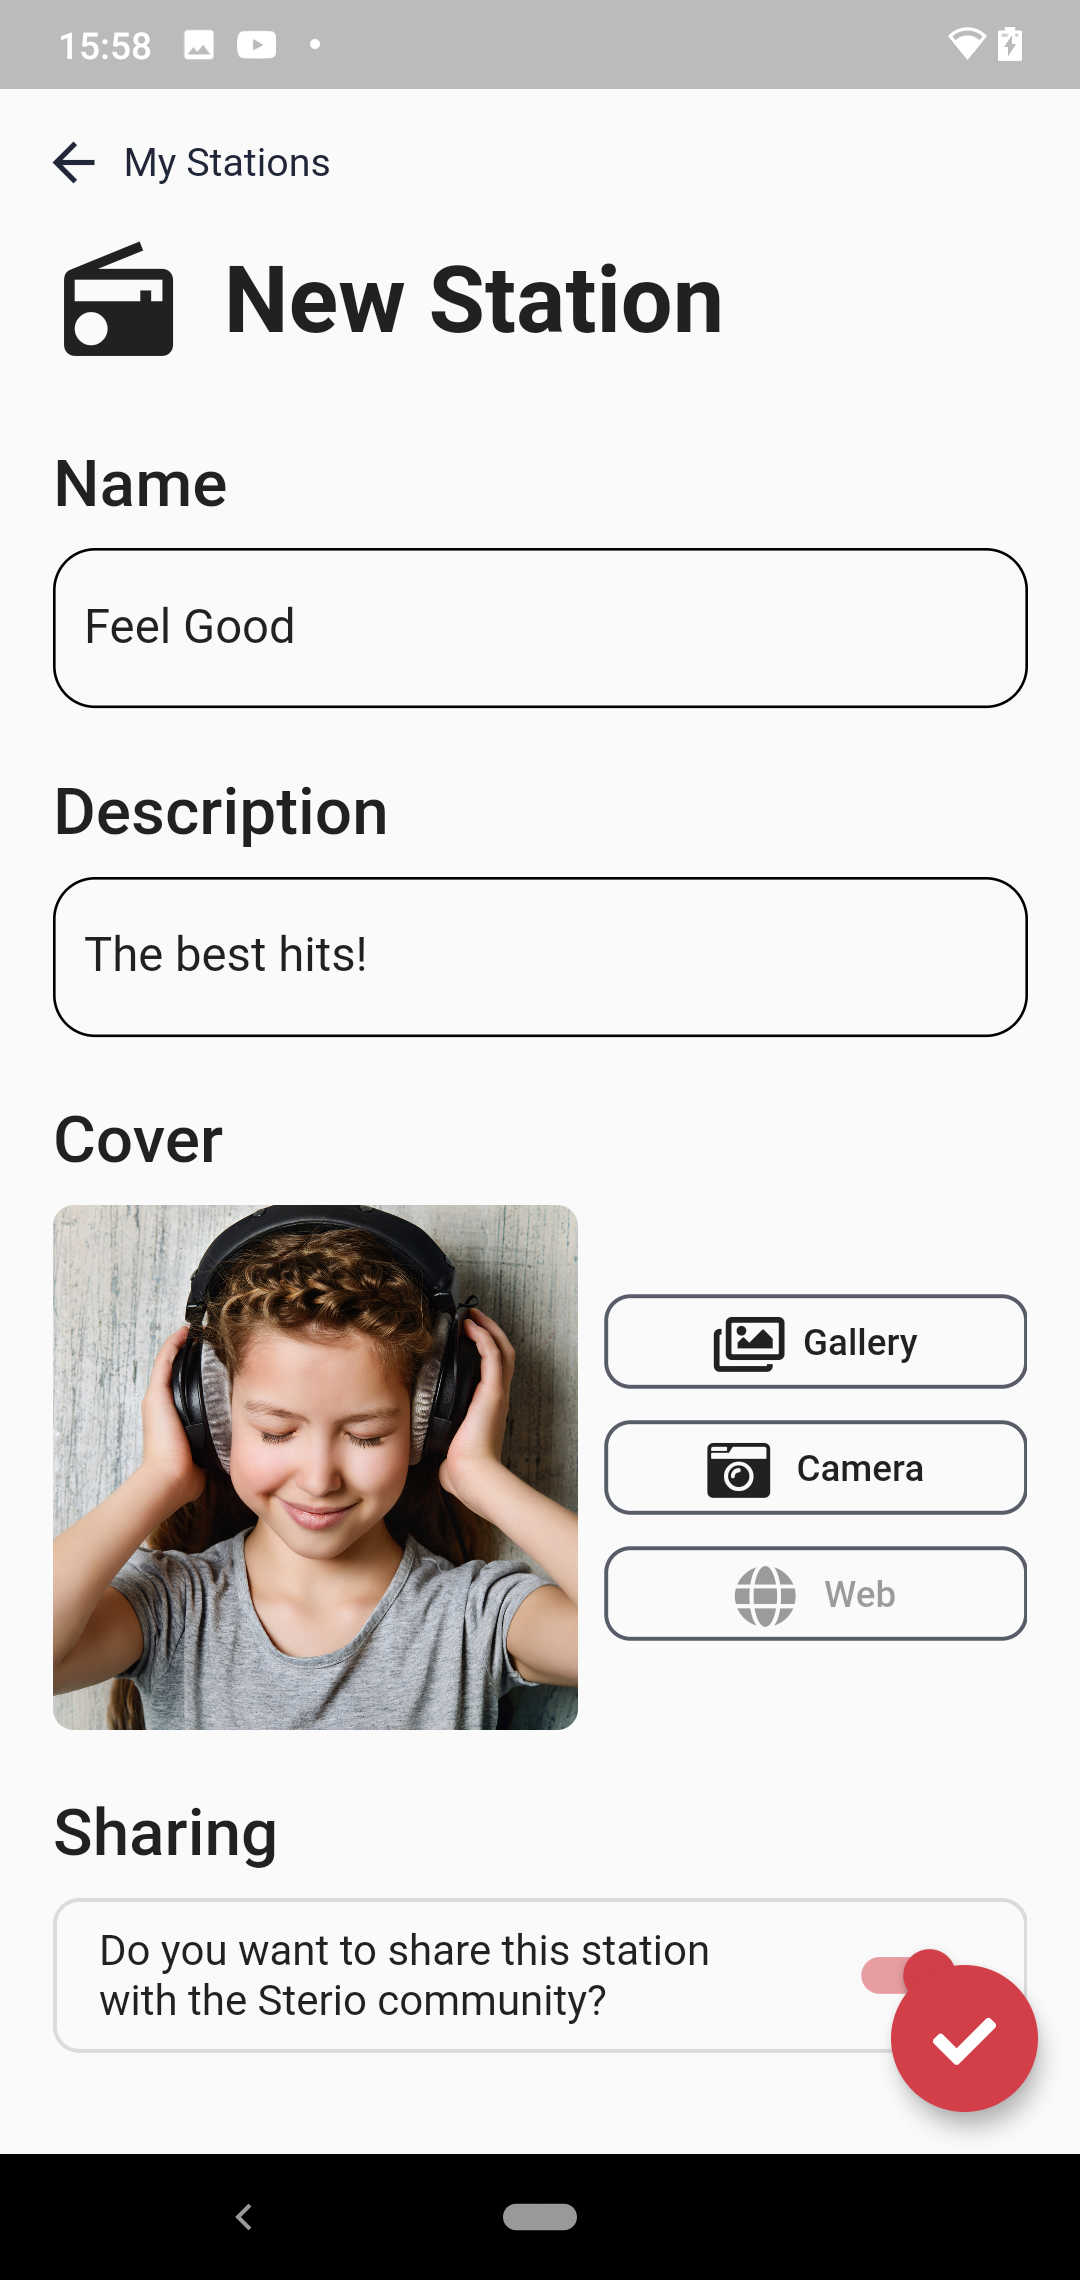
\includegraphics[width=0.29\textwidth]{./Images/screenshots/newstation1.png}}} \qquad
	\subfigure[Step 2 (adding blocks)]{\label{fig:ns2}
	\frame{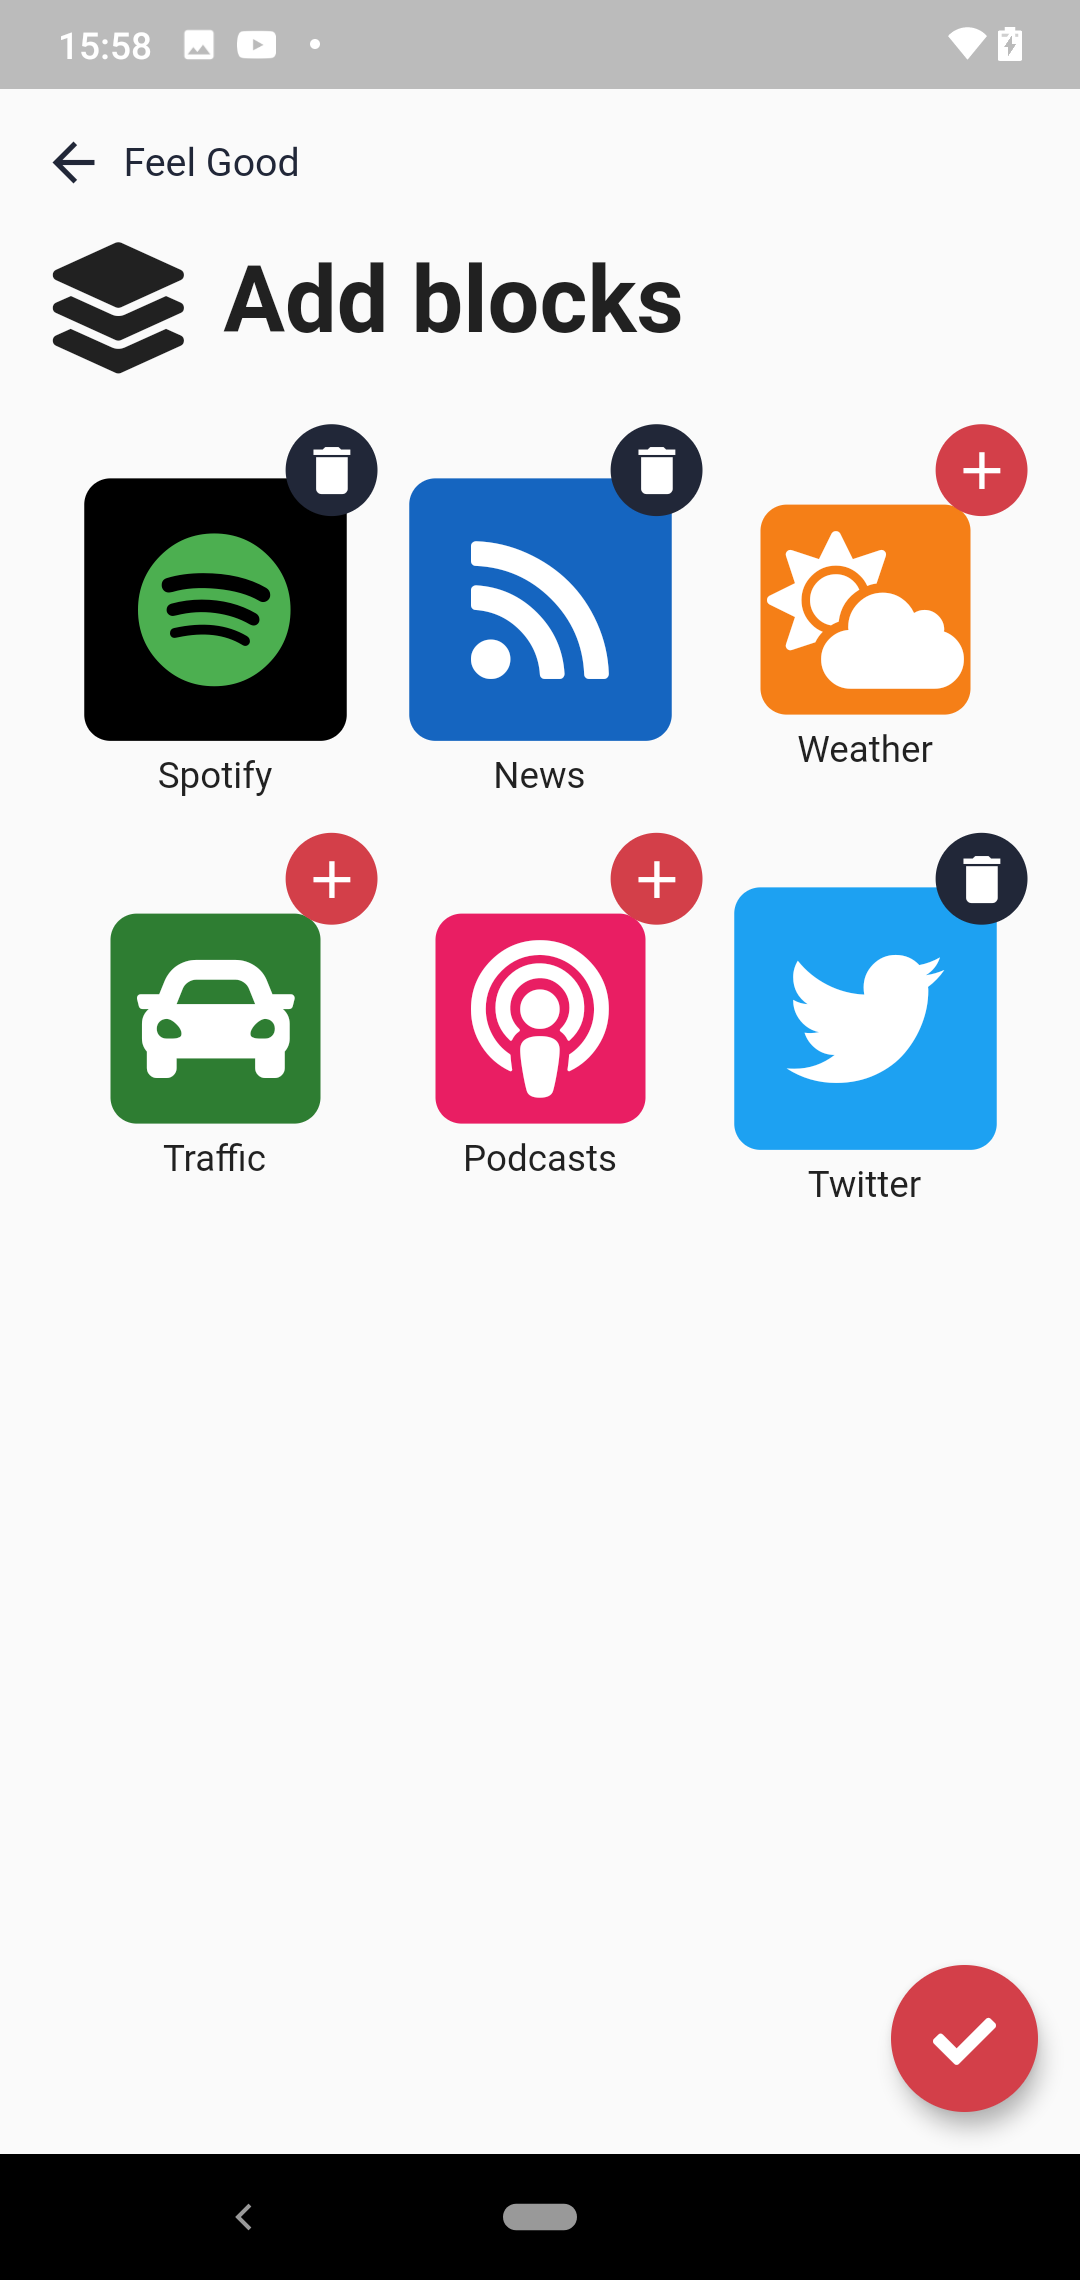
\includegraphics[width=0.29\textwidth]{./Images/screenshots/newstation2.png}}} \qquad
	\subfigure[Success screen]{\label{fig:ns3}
	\frame{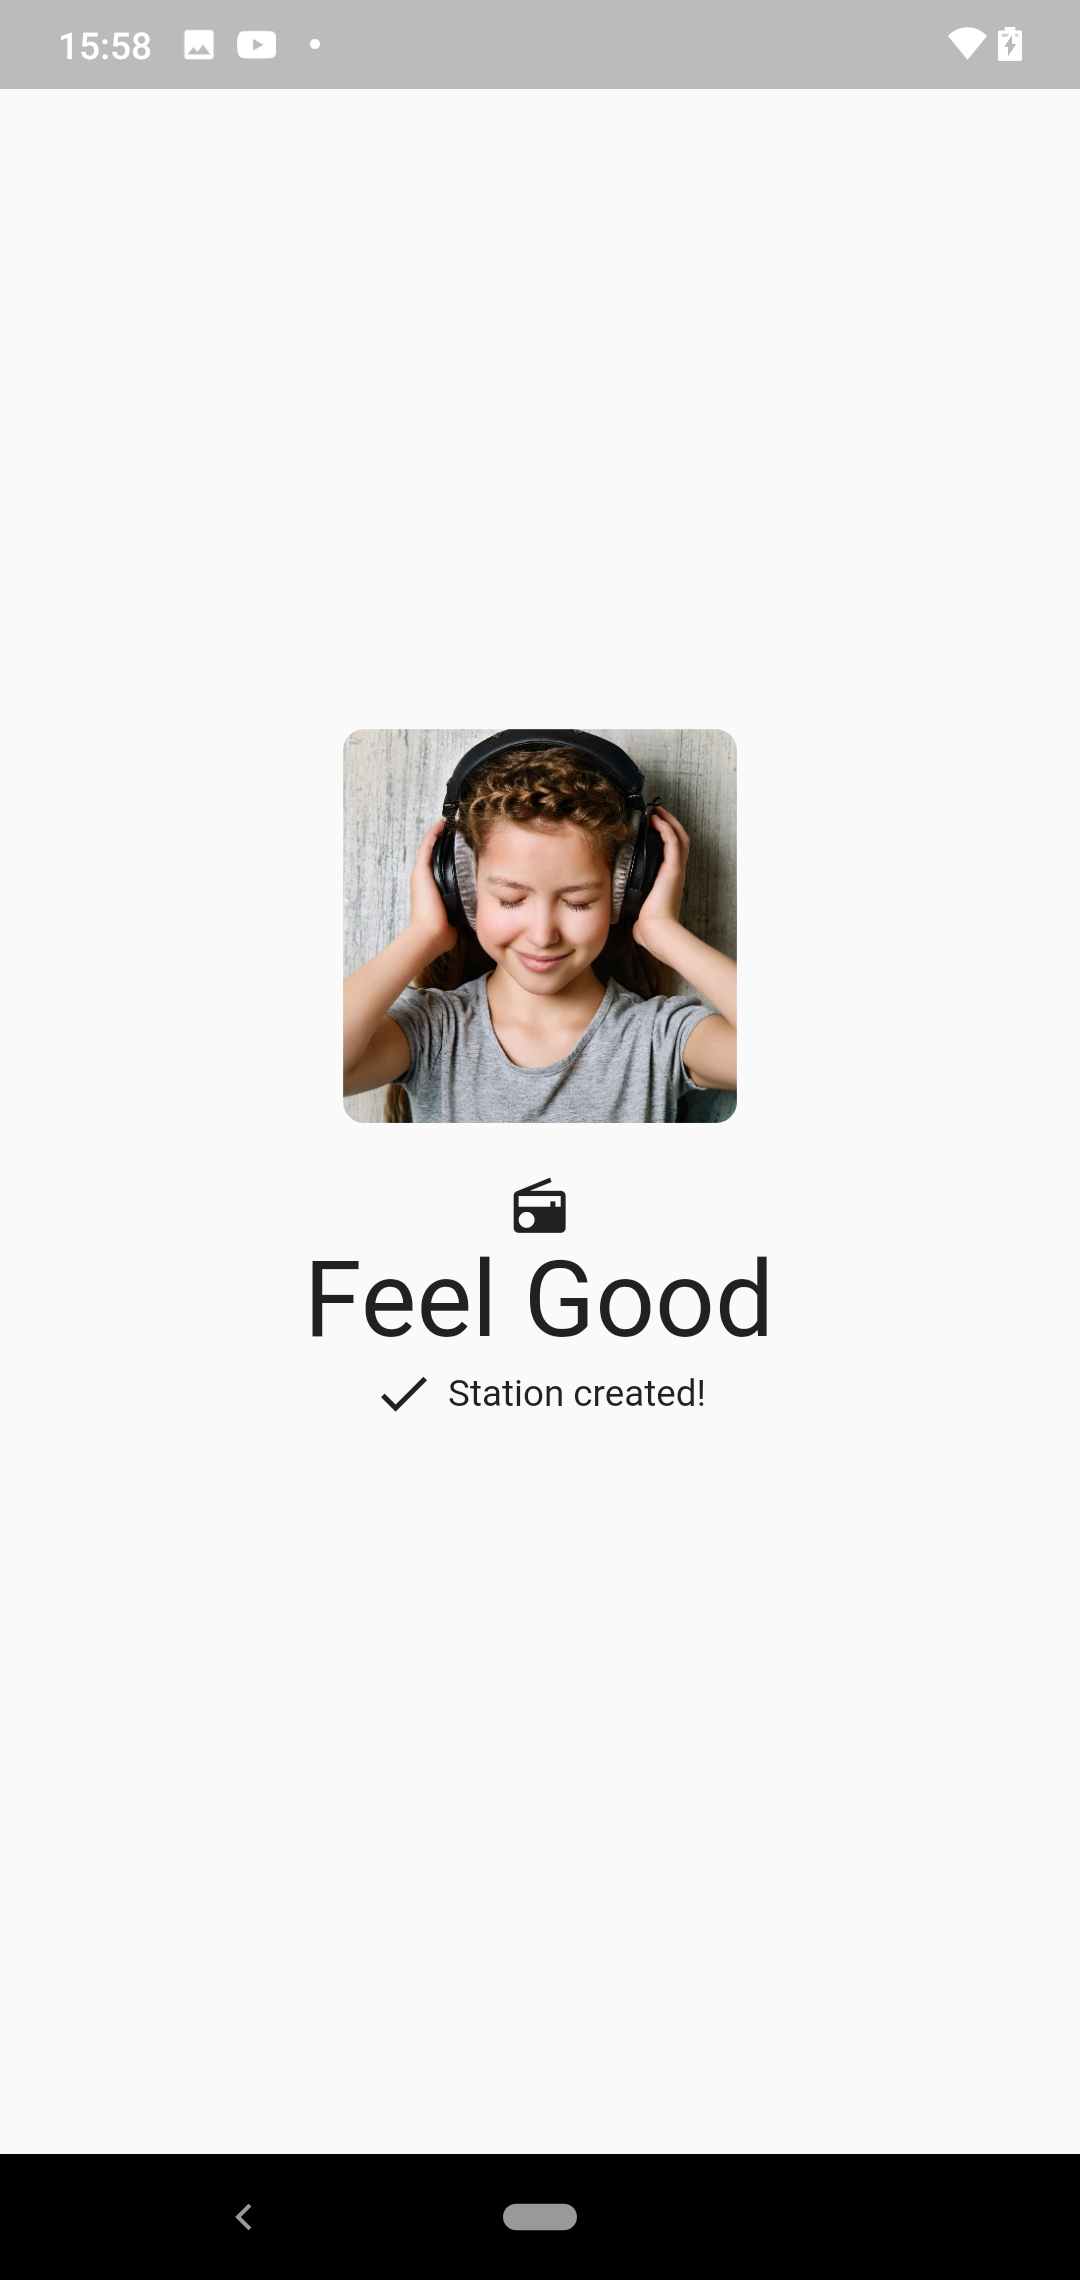
\includegraphics[width=0.29\textwidth]{./Images/screenshots/newstation3.png}}} \qquad
	\caption{Screenshots of the process of creating a new station }
	\label{fig:mfp1}
\end{figure}

From the 'My Stations' screen, users can create their custom stations. This is a simple two-step process  — first, users are requested to enter the name of the station, a brief description, a cover artwork (which can be selected from the local photo gallery, from a web search, or even from taking a picture in real-time), and a sharing option. The latter determines if the station will be kept private to the user (other users can't see the station contents nor play it), or if it is shared with the community of the platform's users. The screen where the user is prompted to enter this information is shown in Figure ~\ref{fig:ns1}.


The second and final step of the creation process of a new station is the selection of 'blocks'. Each 'block' represents a service or source of information that can be added to the station playback. A simple screen, represented in Figure ~\ref{fig:ns2}, is shown to the user so that they can select the desired blocks simply and intuitively. After the user is elated with their choices, the created station information is stored in the database, and if such a process is successful, a confirmation screen  (represented in Figure ~\ref{fig:ns3}) is shown to the user. Finally, the user is redirected to the 'My Stations' screen (Figure ~\ref{fig:mys}), where the newly created station is now listed.

\newpage
\subsection{Configuring and Customizing a Station}

\begin{figure}[htbp]
	\centering
	\subfigure[Blocks screen]{\label{fig:s1}
	\frame{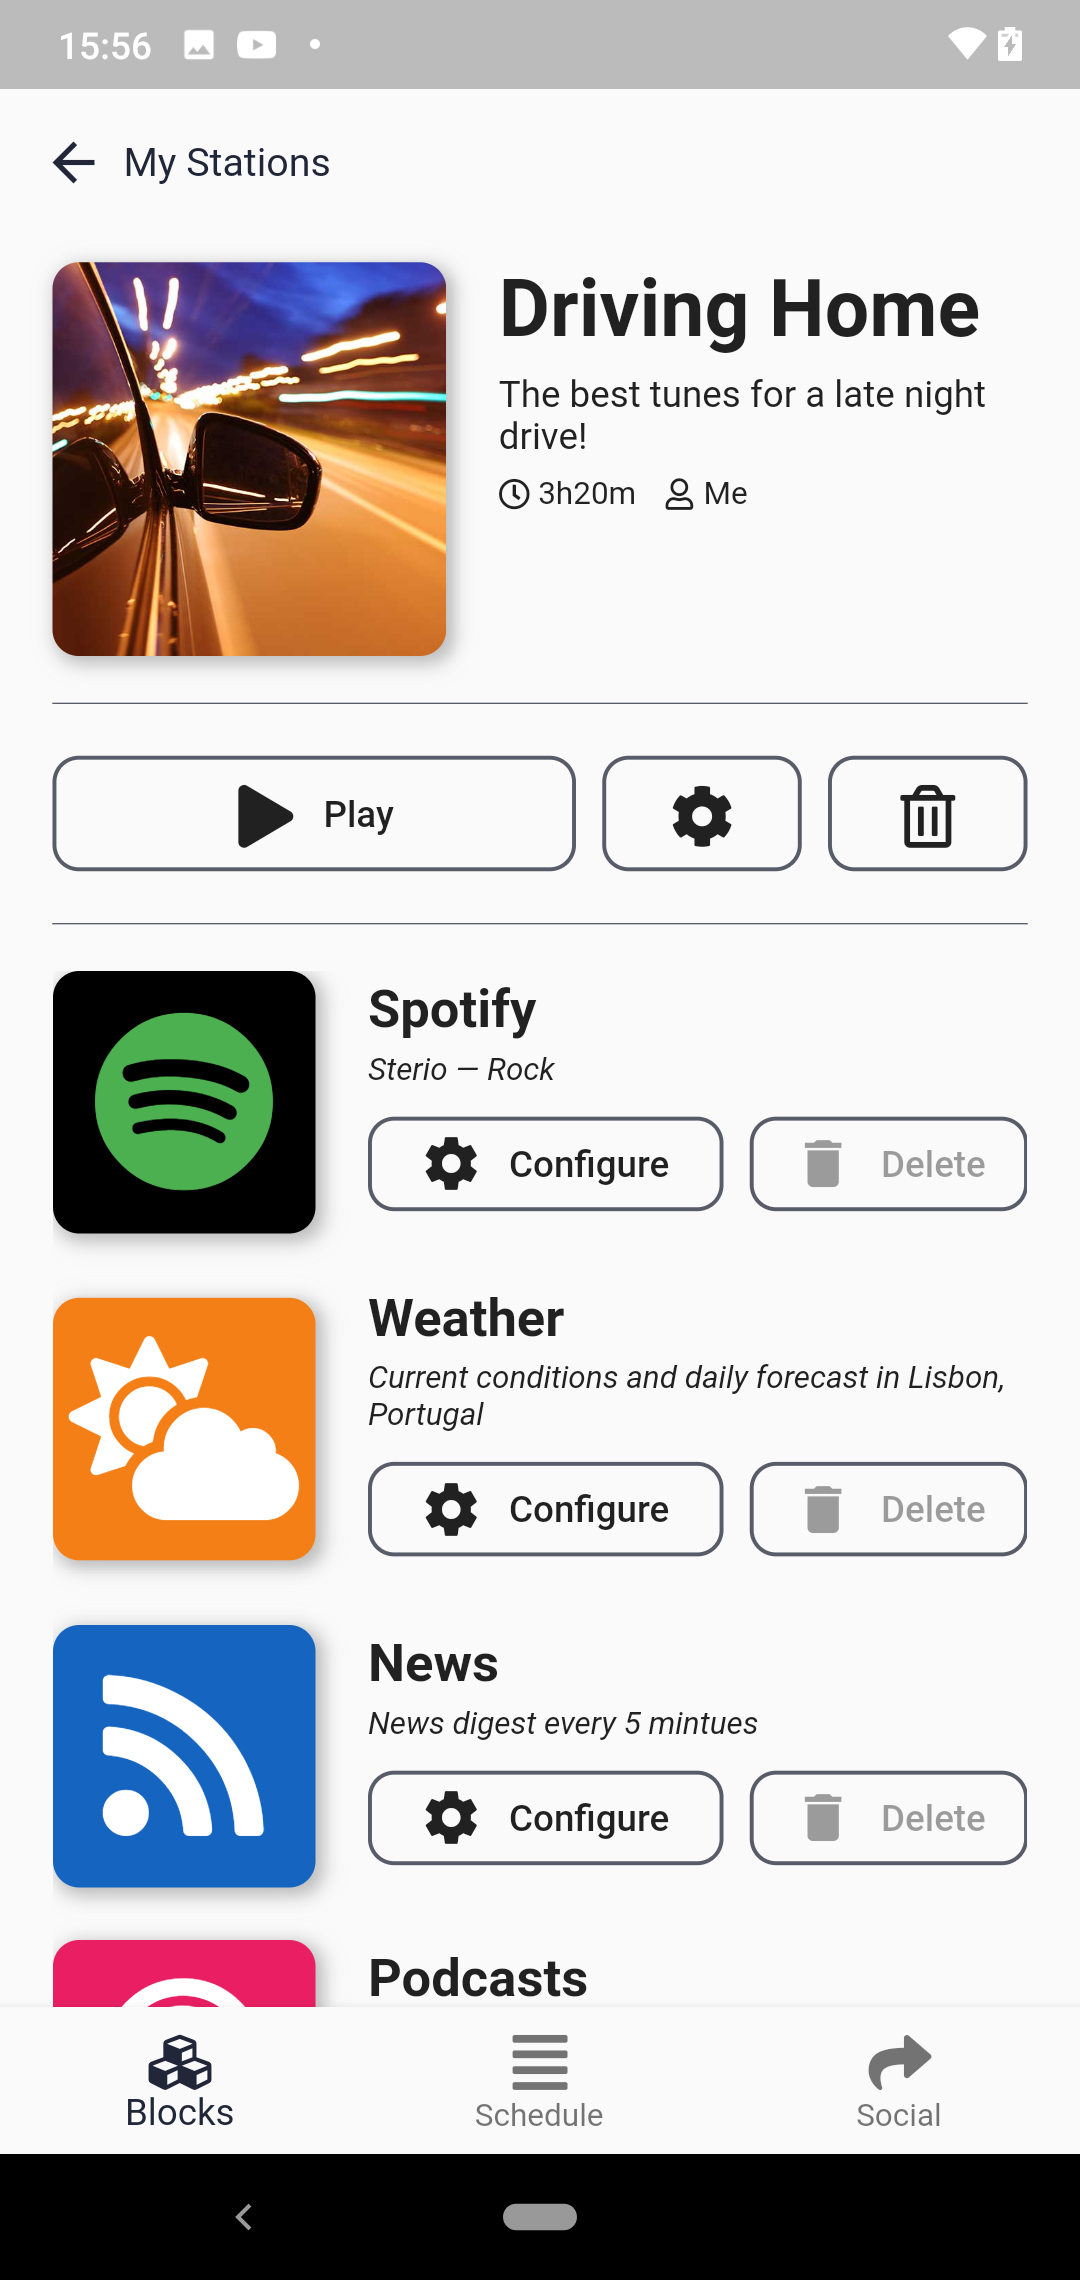
\includegraphics[width=0.29\textwidth]{./Images/screenshots/station1.png}}} \qquad
	\subfigure[Schedule screen screen]{\label{fig:s2}
	\frame{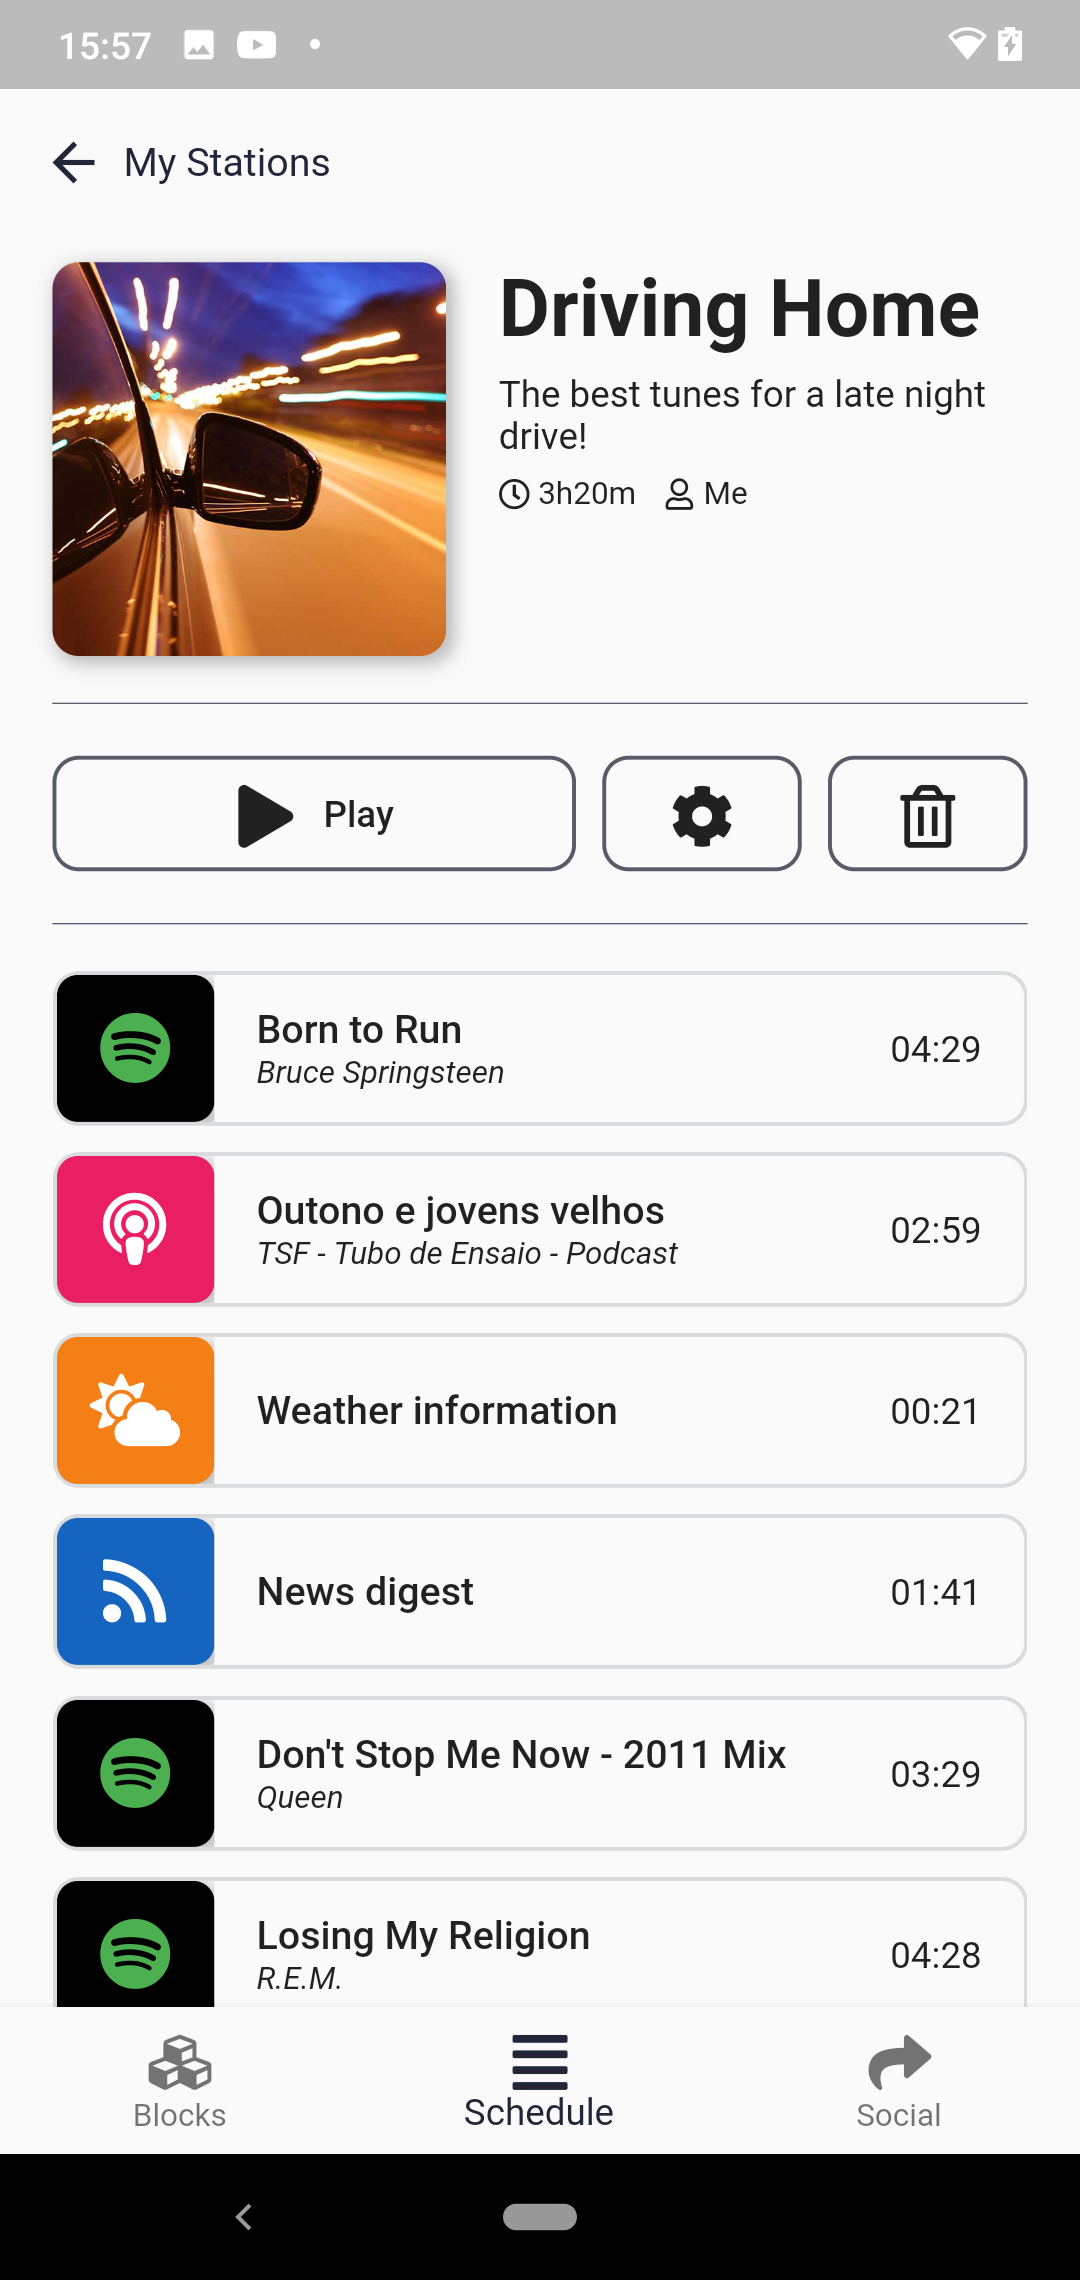
\includegraphics[width=0.29\textwidth]{./Images/screenshots/station2.png}}} \qquad
	\caption{'Driving Home' station screens}
	\label{fig:mfp1}
\end{figure}



Each station has its dedicated page, where the user can explore and customize all aspects and features of it. This screen is divided into three sub-screens that fill the latter half of the canvas — the 'blocks', 'schedule', and 'social' screen.

The 'blocks' screen showcases all the added blocks of the station. In this sub-screen, it is possible to configure, add, or remove individual blocks. The 'schedule' screen presents visually the order in which the content inserted from each block will be played. The user can fully customize the order and also remove individual elements. Finally, in the 'social' screen — which is only displayed if the creator of the station allowed its sharing with the community — users can see the profiles that follow the station, as well to accept or decline any changes that other users have suggested to the station's content.

On the first half of the screen, users can examine the station's name, description, artwork cover, duration, and creator (or creators). There, users can also start playing the station, enter its settings screen (where it is possible to adjust some configurations, such as the used text-to-speech voice), or delete the given station.

In the following subsections, we explain in greater detail the logical and technical implementations of four of the available station blocks — Spotify, Podcasts, Weather, and News. 


\subsubsection{Spotify and Podcasts}
\label{sub:spotify}

The Spotify block serves as the main connection to the music streaming service. From there, users can explore their music library and select their desired content (that could be represented in the form of a single song, artist, album, or even full playlists). To make it easier for users to add content, the recently played songs from the user's Spotify account are also displayed. Users can select an unlimited number of items, which are added to the station schedule automatically and in the order of their choice.

As mentioned in Section ~\ref{chap:relatedwork}, Spotify also provides access to a growing library of podcasts, which the user can also add to their stations. Nevertheless, although the provider of both music and podcasts is the mentioned music streaming service, a separate block dedicated to Podcasts was created.

\begin{figure}[htbp]
	\centering
	\subfigure[Spotify main configuration screen]{\label{fig:spotify1}
	\frame{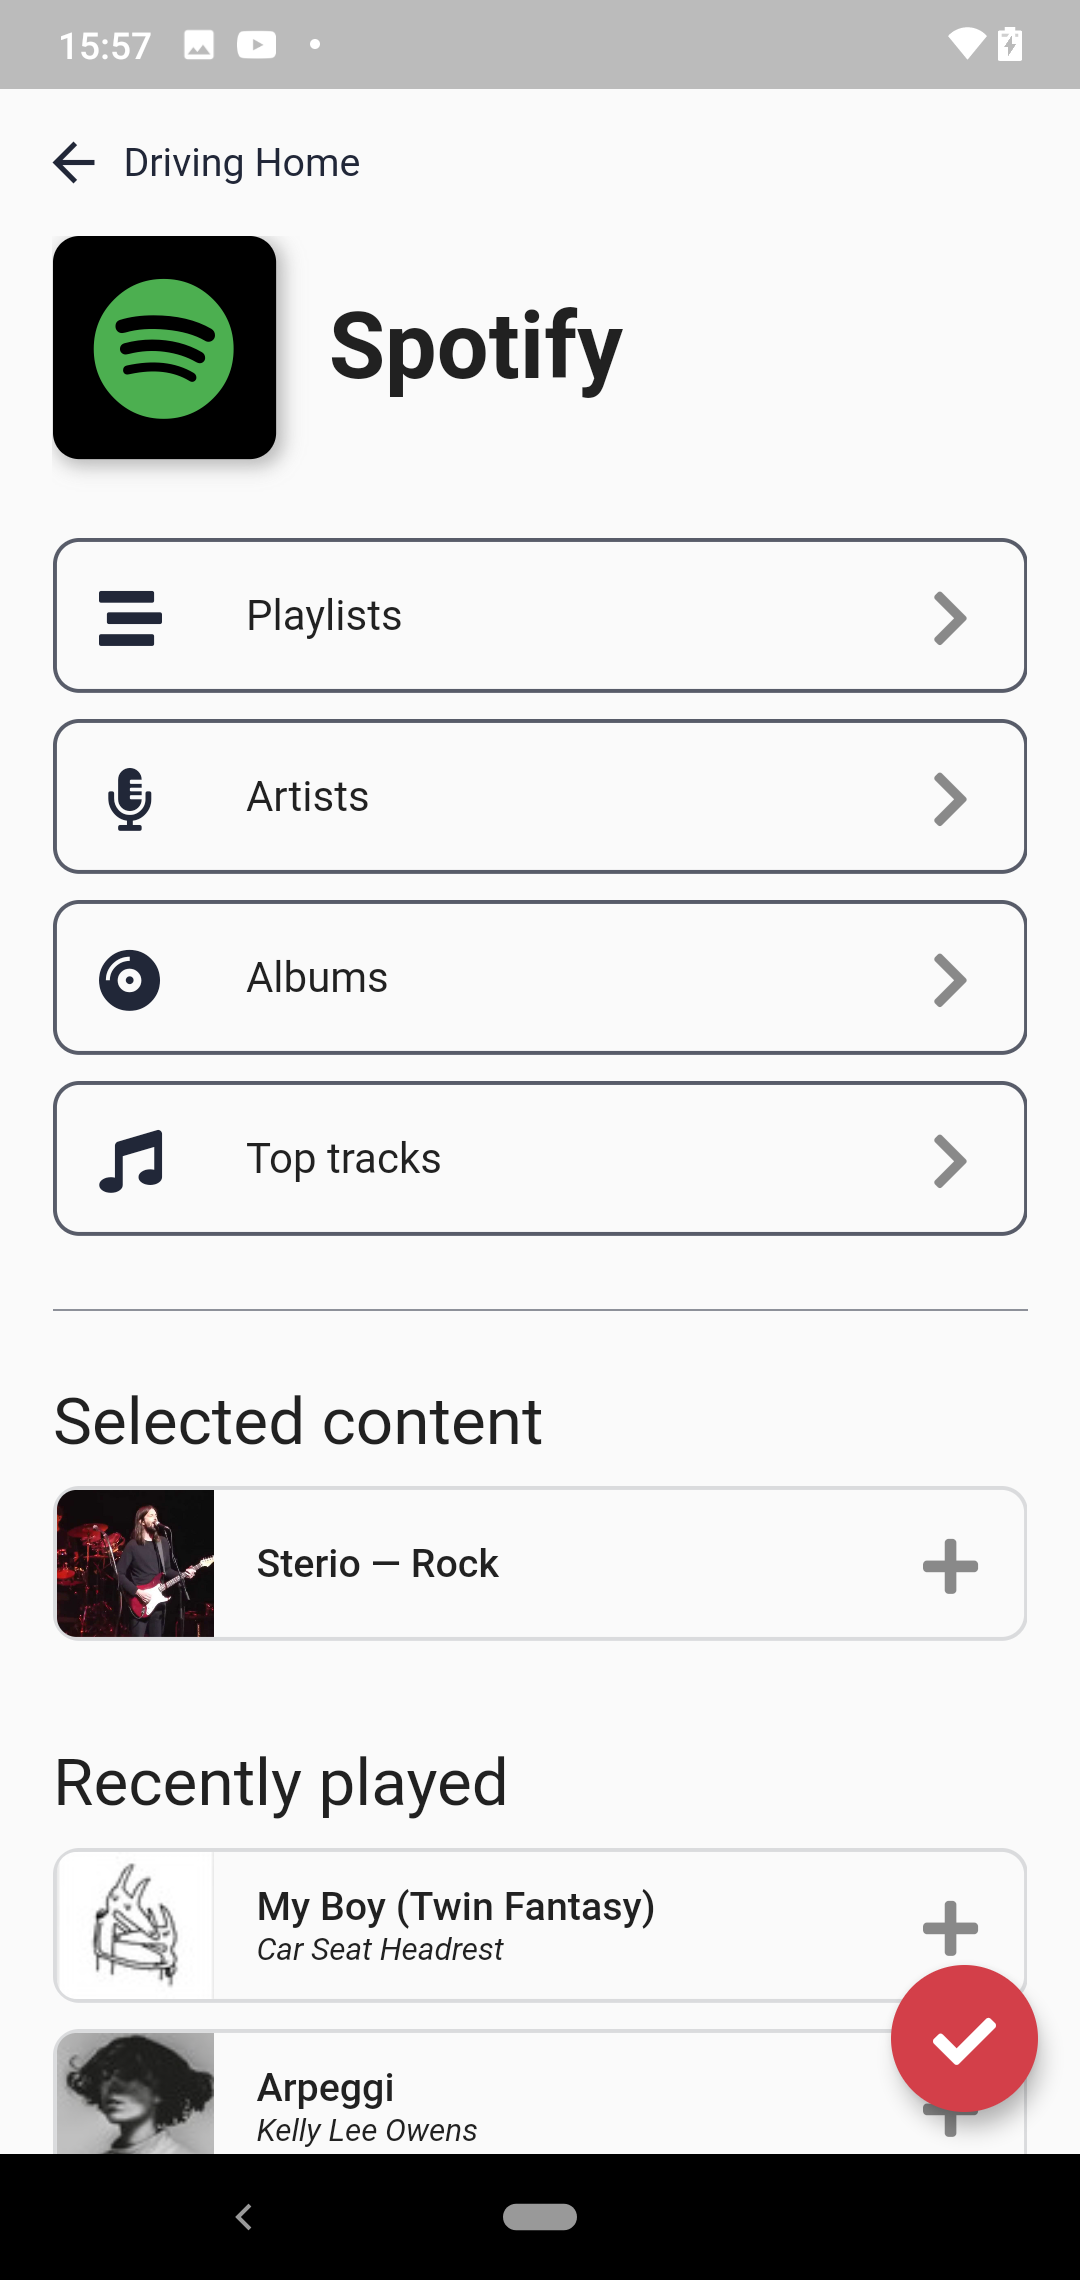
\includegraphics[width=0.29\textwidth]{./Images/screenshots/spotify.png}}} \qquad
	\subfigure[Playlists selection screen]{\label{fig:spotify2}
	\frame{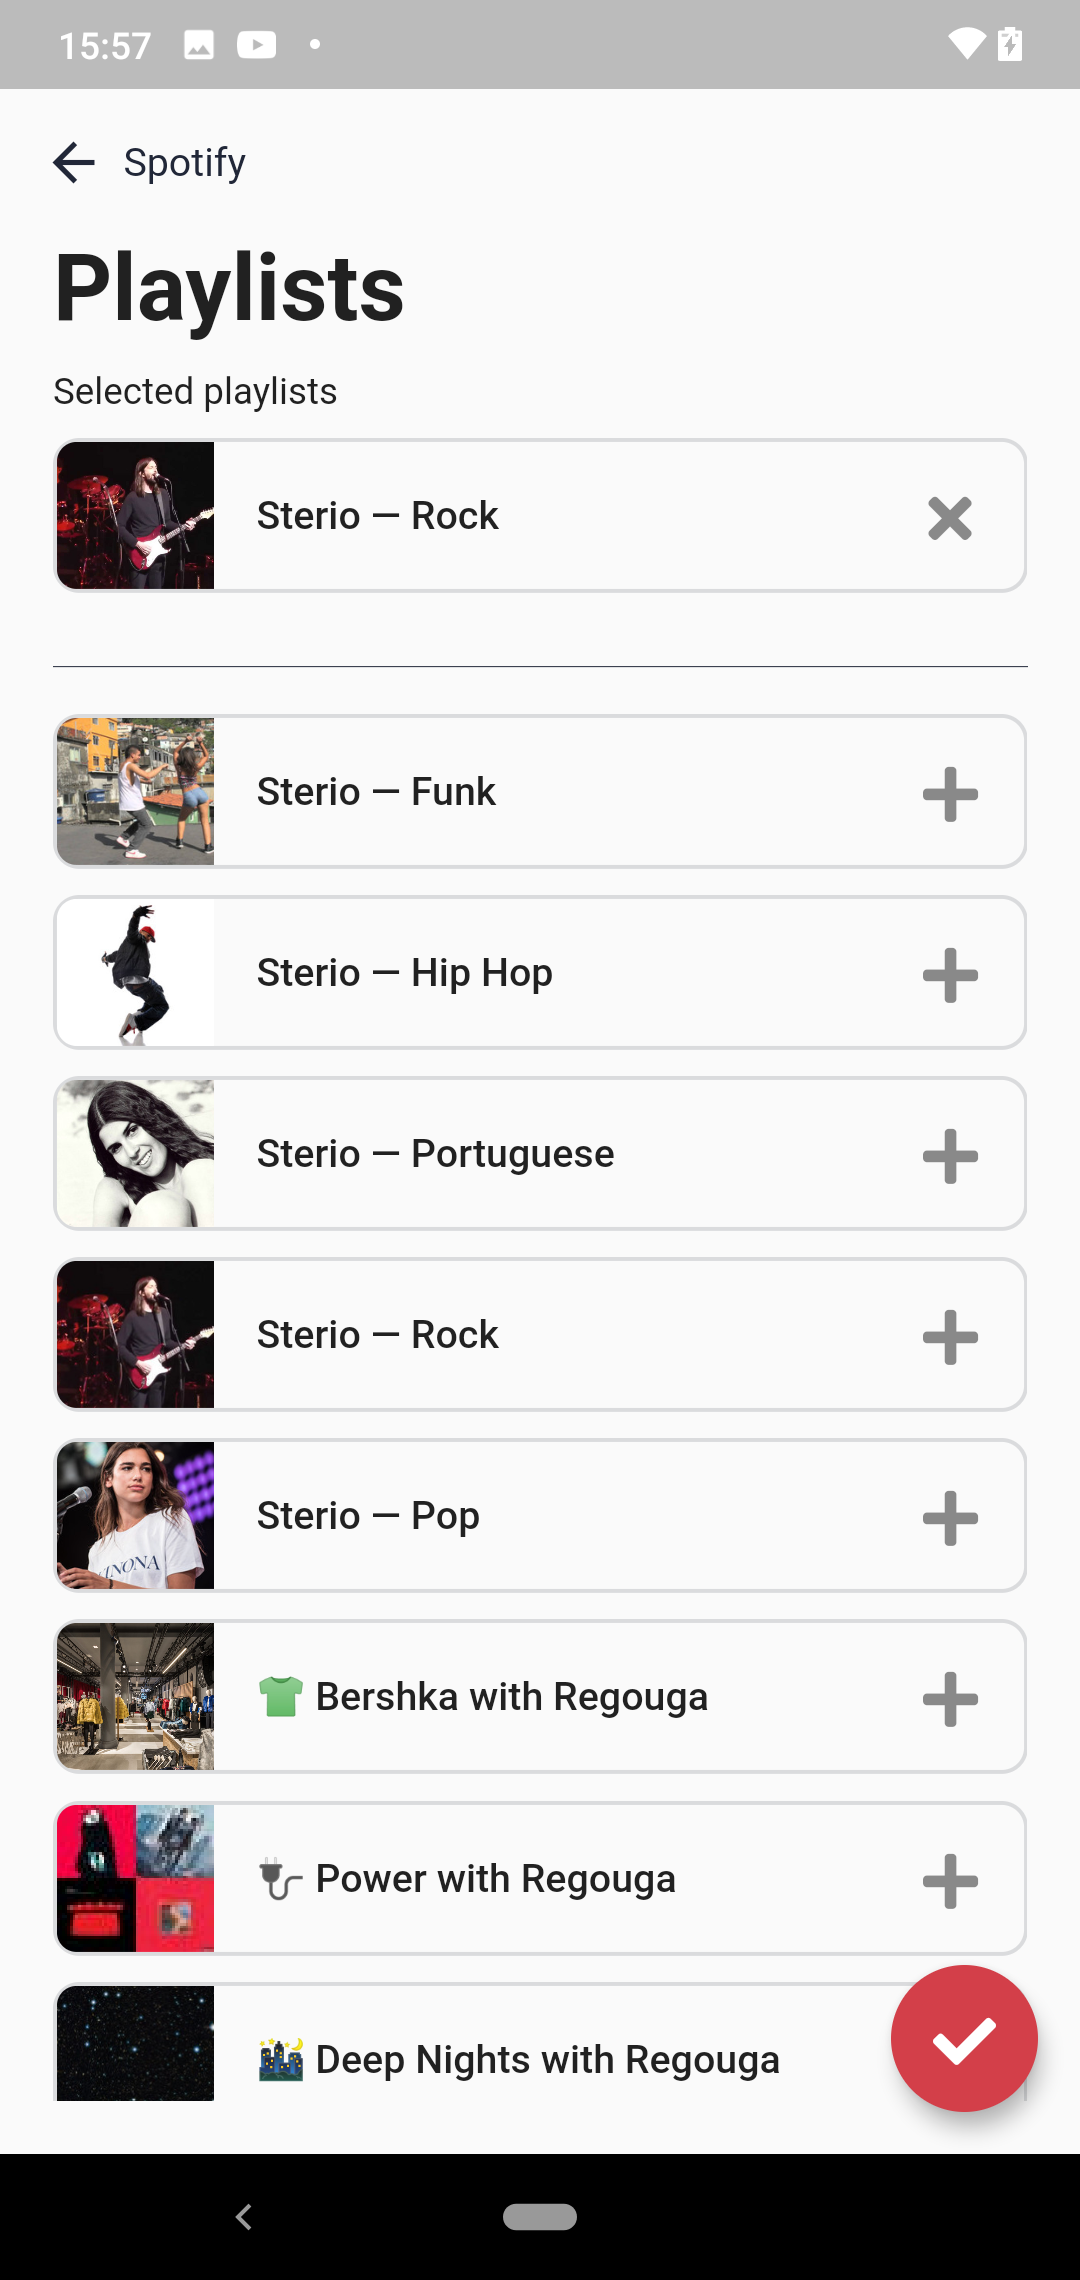
\includegraphics[width=0.29\textwidth]{./Images/screenshots/playlists.png}}} \qquad
	\caption{Spotify block configuration screens}
	\label{fig:spp1}
\end{figure}

Each item (song, album, playlist, artist, or podcast) is represented by a unique \ac{URI}, which are obtained with the resource to the Spotify Web \ac{API} ~\footnote{For more information on the development resources provided by Spotify, visit the \href{https://developer.spotify.com/documentation/web-api/}{Spotify for Developers website}}. The credentials entered by the user (described in Section ~\ref{subsec:lsa}) are used to authenticate and make an API call requesting the desired information. A response JSON file is sent to the backend, where it is processed and, afterward, the information is presented to the user, where they can add the desired content to the station.

\begin{figure}[h]
\centering
\frame{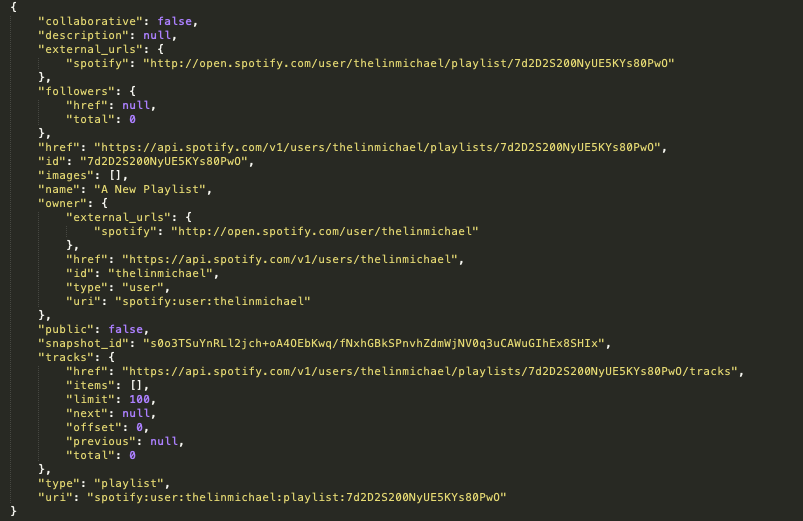
\includegraphics[width=0.8\textwidth]{./Images/code/jsr.png}}
\caption{Response JSON file of a call to the playlist library of Spotify's Web API}
\label{fig:mys}
\end{figure}


The Spotify Web \ac{API} provides several useful features in the context of our project. For instance, it is possible to search the entire Spotify catalog for a specific element, get curated playlists created by Spotify’s editorial team based on popularity, mood, international events, and genres, or even present the best content recommendations based on a variety of terms such as market, seeds (artists, genres, tracks), ranged audio features (danceability, valence, tempo, liveness) and popularity. In the end, this creates a very integrated and personalized experience for the platform's users.

The selected \acp{URI} are linked to the matching station and stored in the database, so that when a user plays a station, Spotify can gather this information and use it to play an individual item. This algorithm — that uses Spotify's Playback \ac{API}, rather than the Web \ac{API} — is further explained in detail in Section ~\ref{subs:playing}.
\newpage

\subsubsection{Weather}

\begin{figure}[htbp]
	\centering
	\subfigure[Main configuration screen]{\label{fig:news1}
	\frame{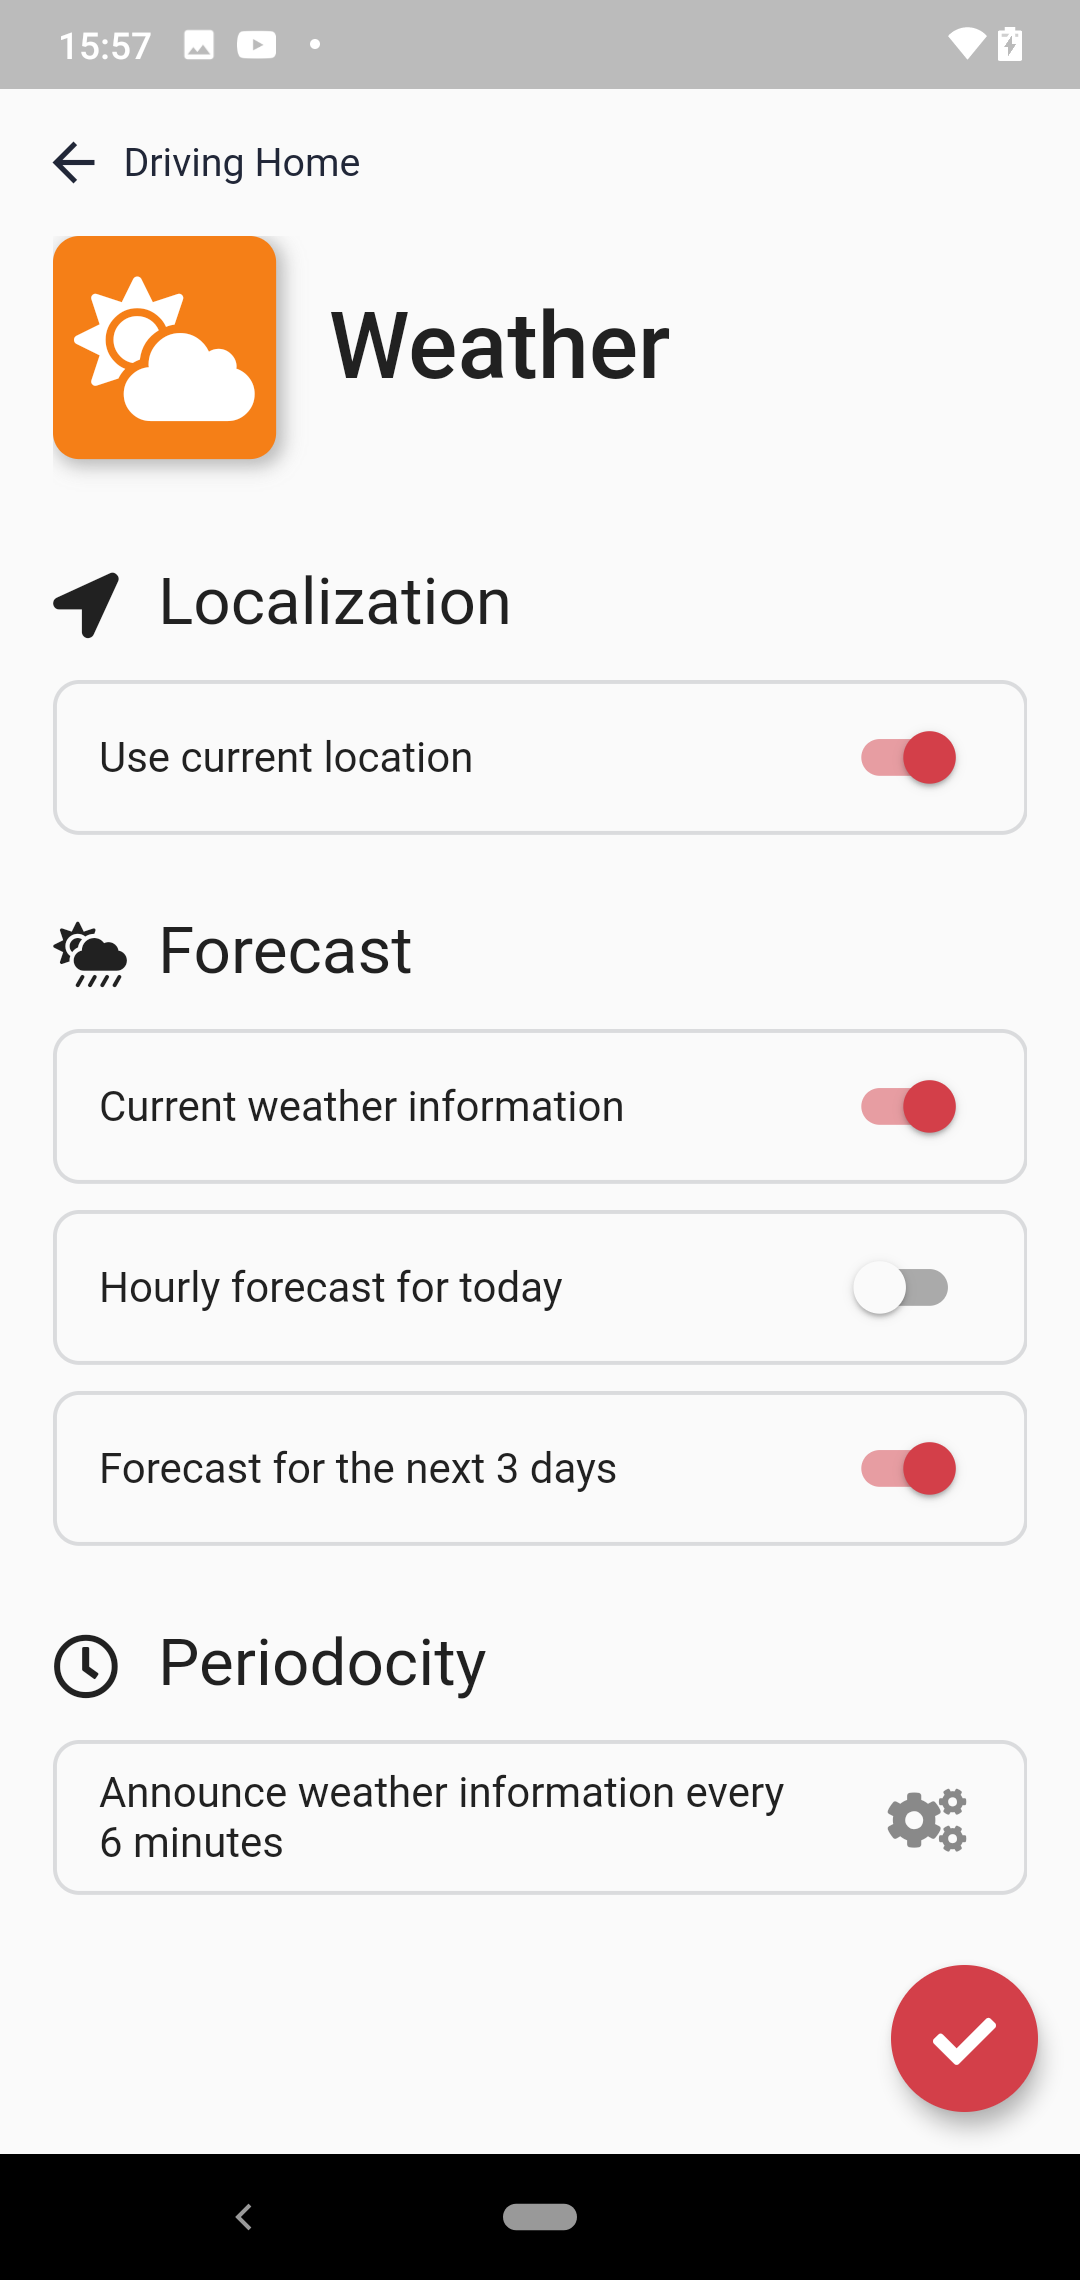
\includegraphics[width=0.29\textwidth]{./Images/screenshots/weather.png}}} \qquad
	\subfigure[Dial selector of weather periodicity]{\label{fig:news2}
	\frame{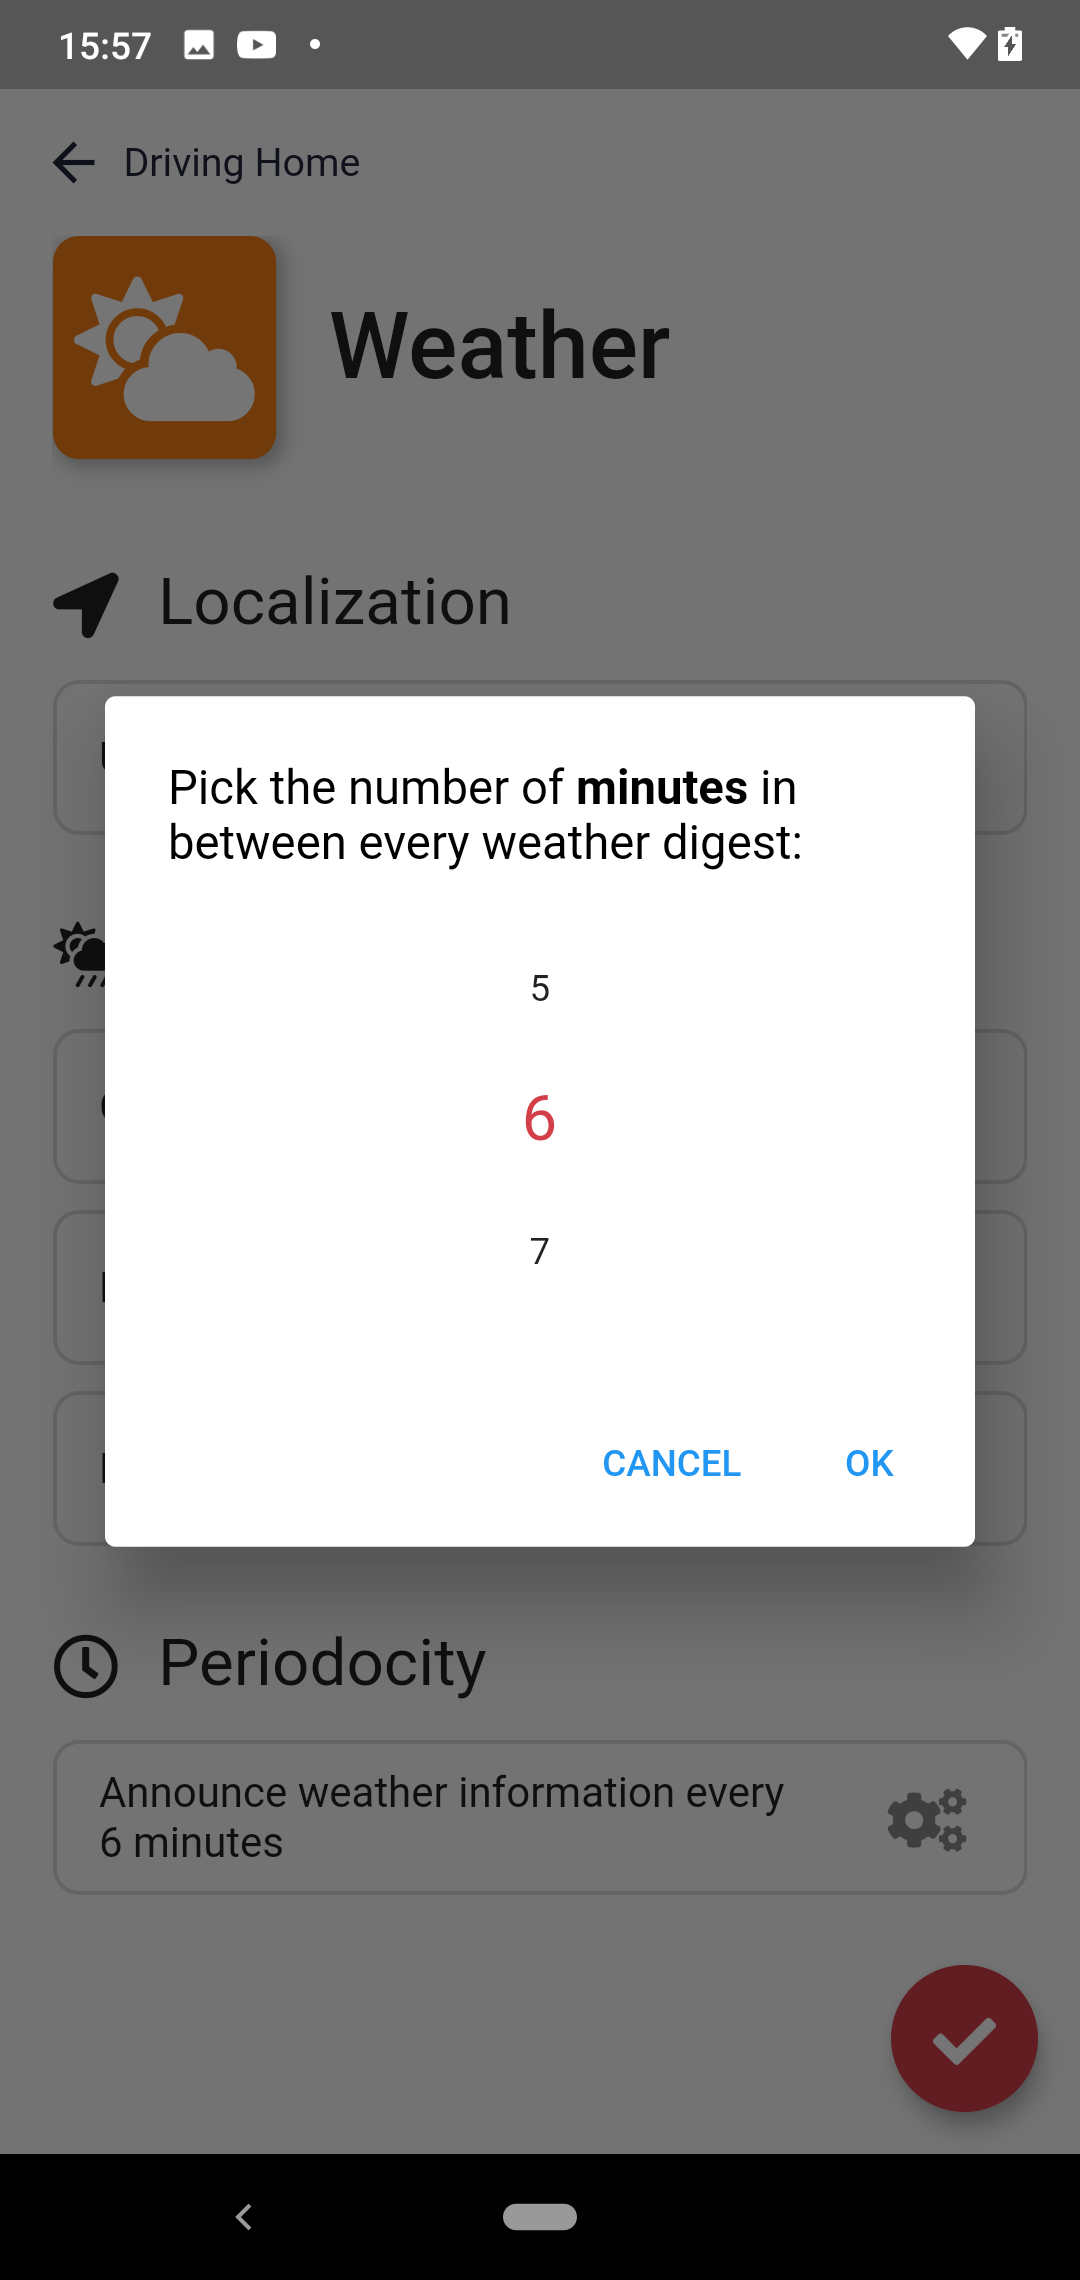
\includegraphics[width=0.29\textwidth]{./Images/screenshots/dial.png}}} \qquad
	\caption{Weather block configuration screens}
	\label{fig:weather}
\end{figure}

The Weather block provides real-time and updated climate information to a given station. Users can choose to listen to the current weather information, hourly forecast for the current day, and/or forecast for the following three days. It is also possible to customize the periodicity of when this information is played in the station, which will change its matching schedule. Finally, users can also set the location from which they want to receive weather information — by default, this is attributed to the user's current location. These settings set by the user are stored in the database.

To gather meteorology information, we rely on the OpenWeather Map \ac{API} ~\footnote{For more information on used API, visit the \href{https://openweathermap.org/api}{OpenWeather API website.}}, which provides the required information reliably and effortlessly. A 'GET' request is made to the \ac{API}, which response is a JSON file containing all the necessary information. 

\newpage
\subsubsection{News}

The News block provides a digest of the top headlines to a given station. Users can select the categories of news they wish to listen to, the number of headlines, and the periodicity of the digest. It is also possible to select a specific keyword to fetch news from (e.g. "COVID-19"), or even select the sources from where the headlines are retrieved. These settings set by the user are also stored in the database.

We used the News \ac{API} to fetch this information, which delivers breaking news headlines, and allows the search for articles from news sources and blogs all over the web~\footnote{For more information on used API, visit the \href{https://newsapi.org/}{News API website.}}. Just like on the Weather block, a 'GET' request is made to the \ac{API}, which response is a JSON file containing all the requested information by the user.

\begin{figure}[htbp]
	\centering
	\subfigure[News categories selection]{\label{fig:news1}
	\frame{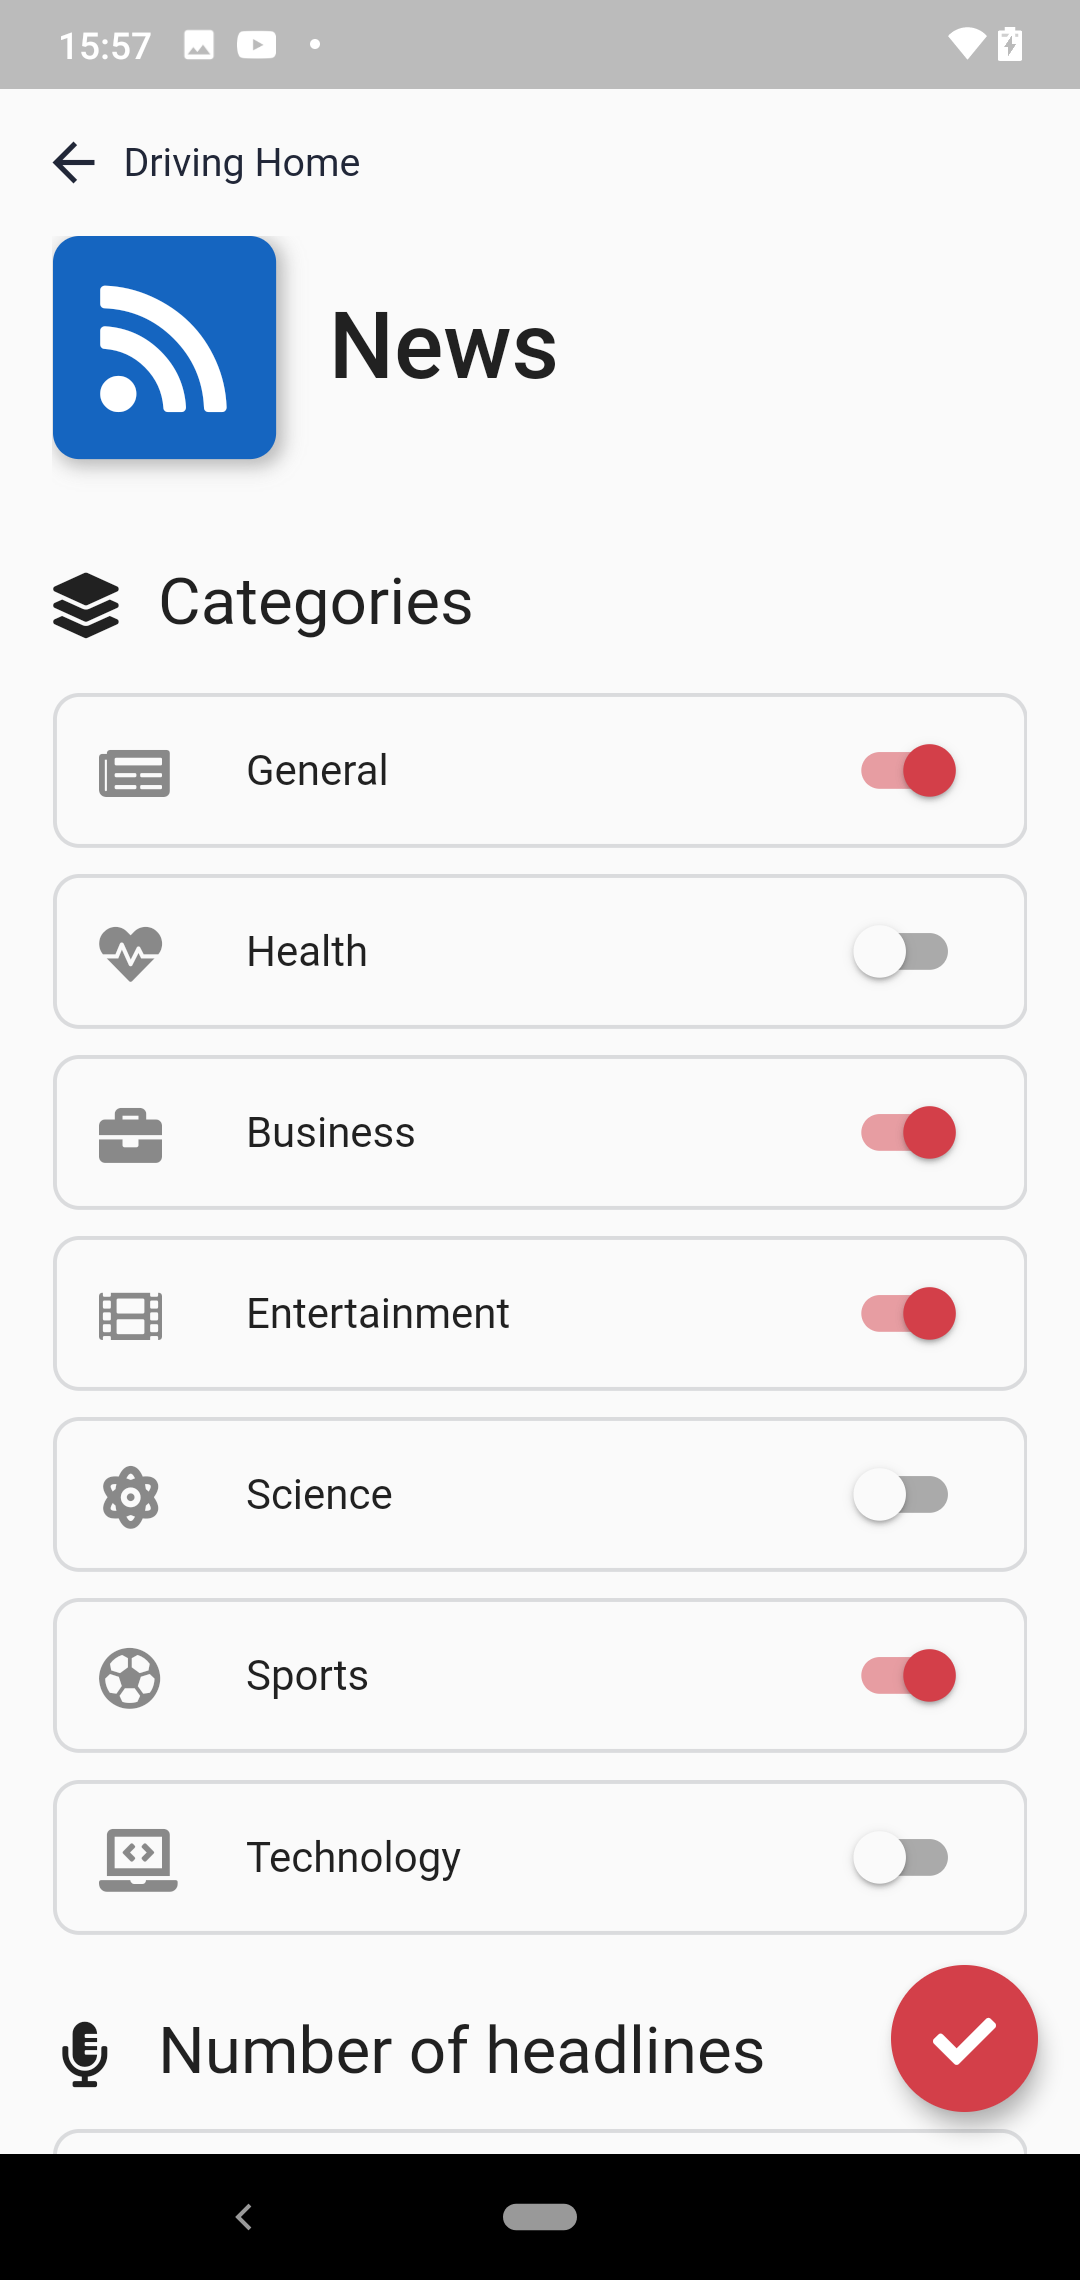
\includegraphics[width=0.29\textwidth]{./Images/screenshots/news1.png}}} \qquad
	\subfigure[Number of headlines and periodocity]{\label{fig:news2}
	\frame{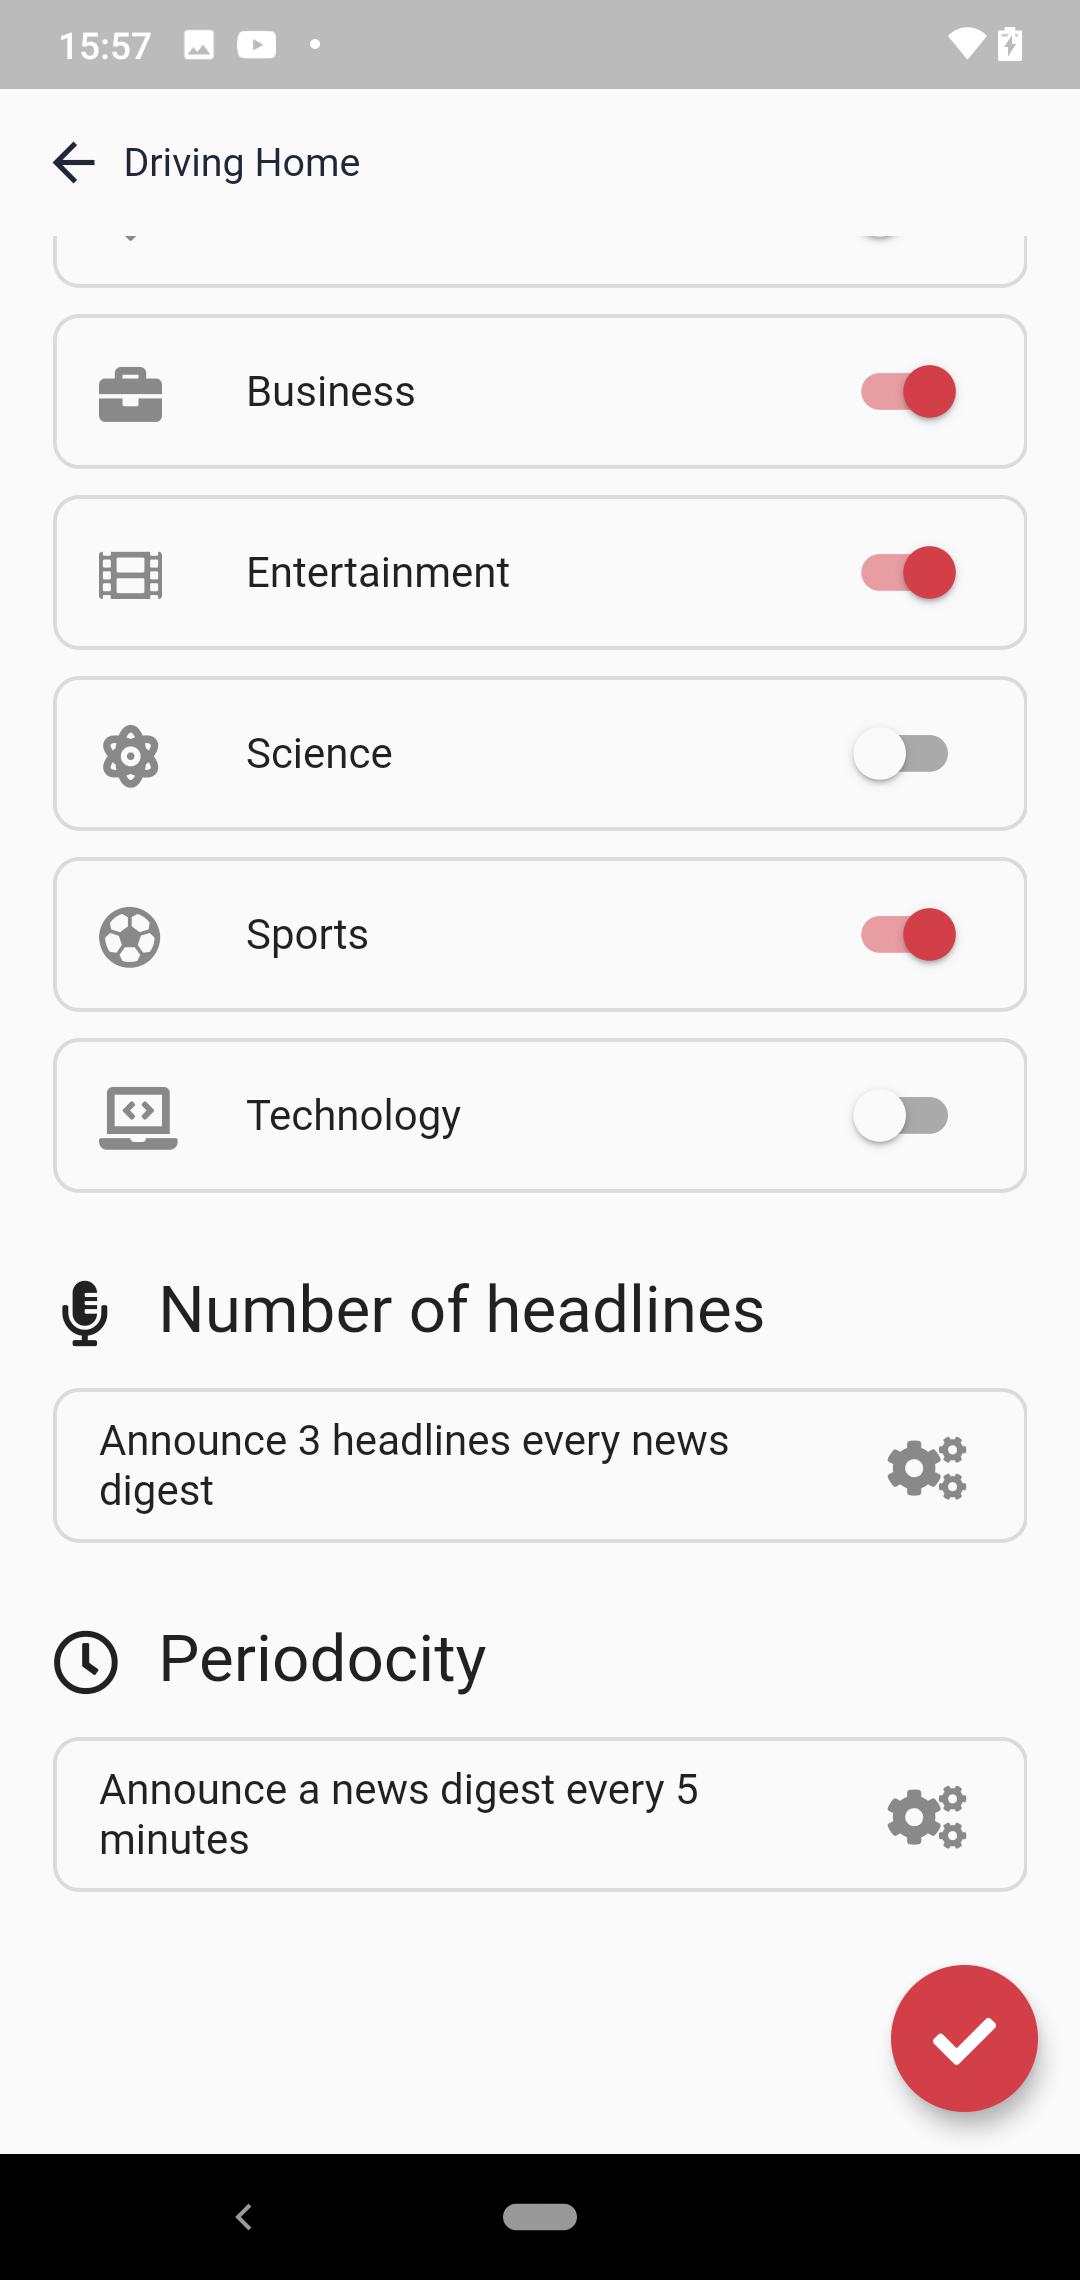
\includegraphics[width=0.29\textwidth]{./Images/screenshots/news2.png}}} \qquad
	\caption{News block configuration screens}
	\label{fig:mfp1}
\end{figure}


When the News block is played in the station, each headline is synthesized and announced by the text-to-speech software, just like any other block containing readable information. To each headline, a small, descriptive block of text is added to provide more context on the news. Then, an audio separator is played, so that the user knows when the announcement of the next headline begun.

The headlines are obtained based on the country and language selected by the user in the signup process of the platform. Nevertheless, the user has full control over this matter and can choose to obtain news headlines from a variety of search terms, topics, countries, languages, and categories.



\begin{figure}[h]
\centering
\frame{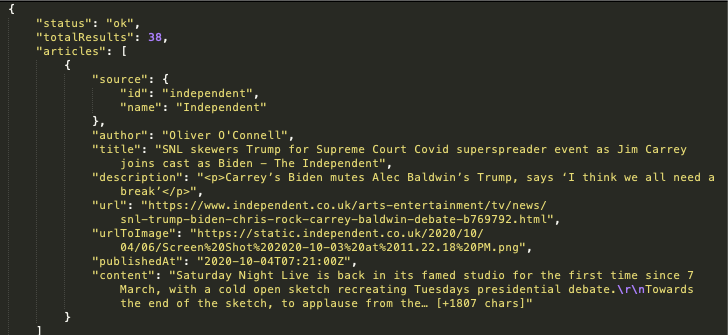
\includegraphics[width=0.8\textwidth]{./Images/code/news.png}}
\caption{Response JSON file of a call to the News API}
\label{fig:mys}
\end{figure}

\newpage
\subsection{Playing a Station}
~\label{subs:playing}

When the station is fully customized to the user's taste, it is then possible to play it. To do so, the user simply needs to tap the 'Play' button, located either at the station information screen or at the preview card displayed on the 'My Stations' screen. 

After tapping the 'Play' button, a modal, represented in Figure ~\ref{fig:play1} is shown to the user, which acts as a 'loading' screen while the backend of the platform performs the necessary tasks to allow the playing of the station. To give a radio-like experience, it is played an audio track that mimics the sounds of tuning into a traditional terrestrial radio station, which automatically stops when all loading processes are complete. 

\begin{figure}[htbp]
	\centering
	\subfigure[Loading ("tuning") screen]{\label{fig:play1}
	\frame{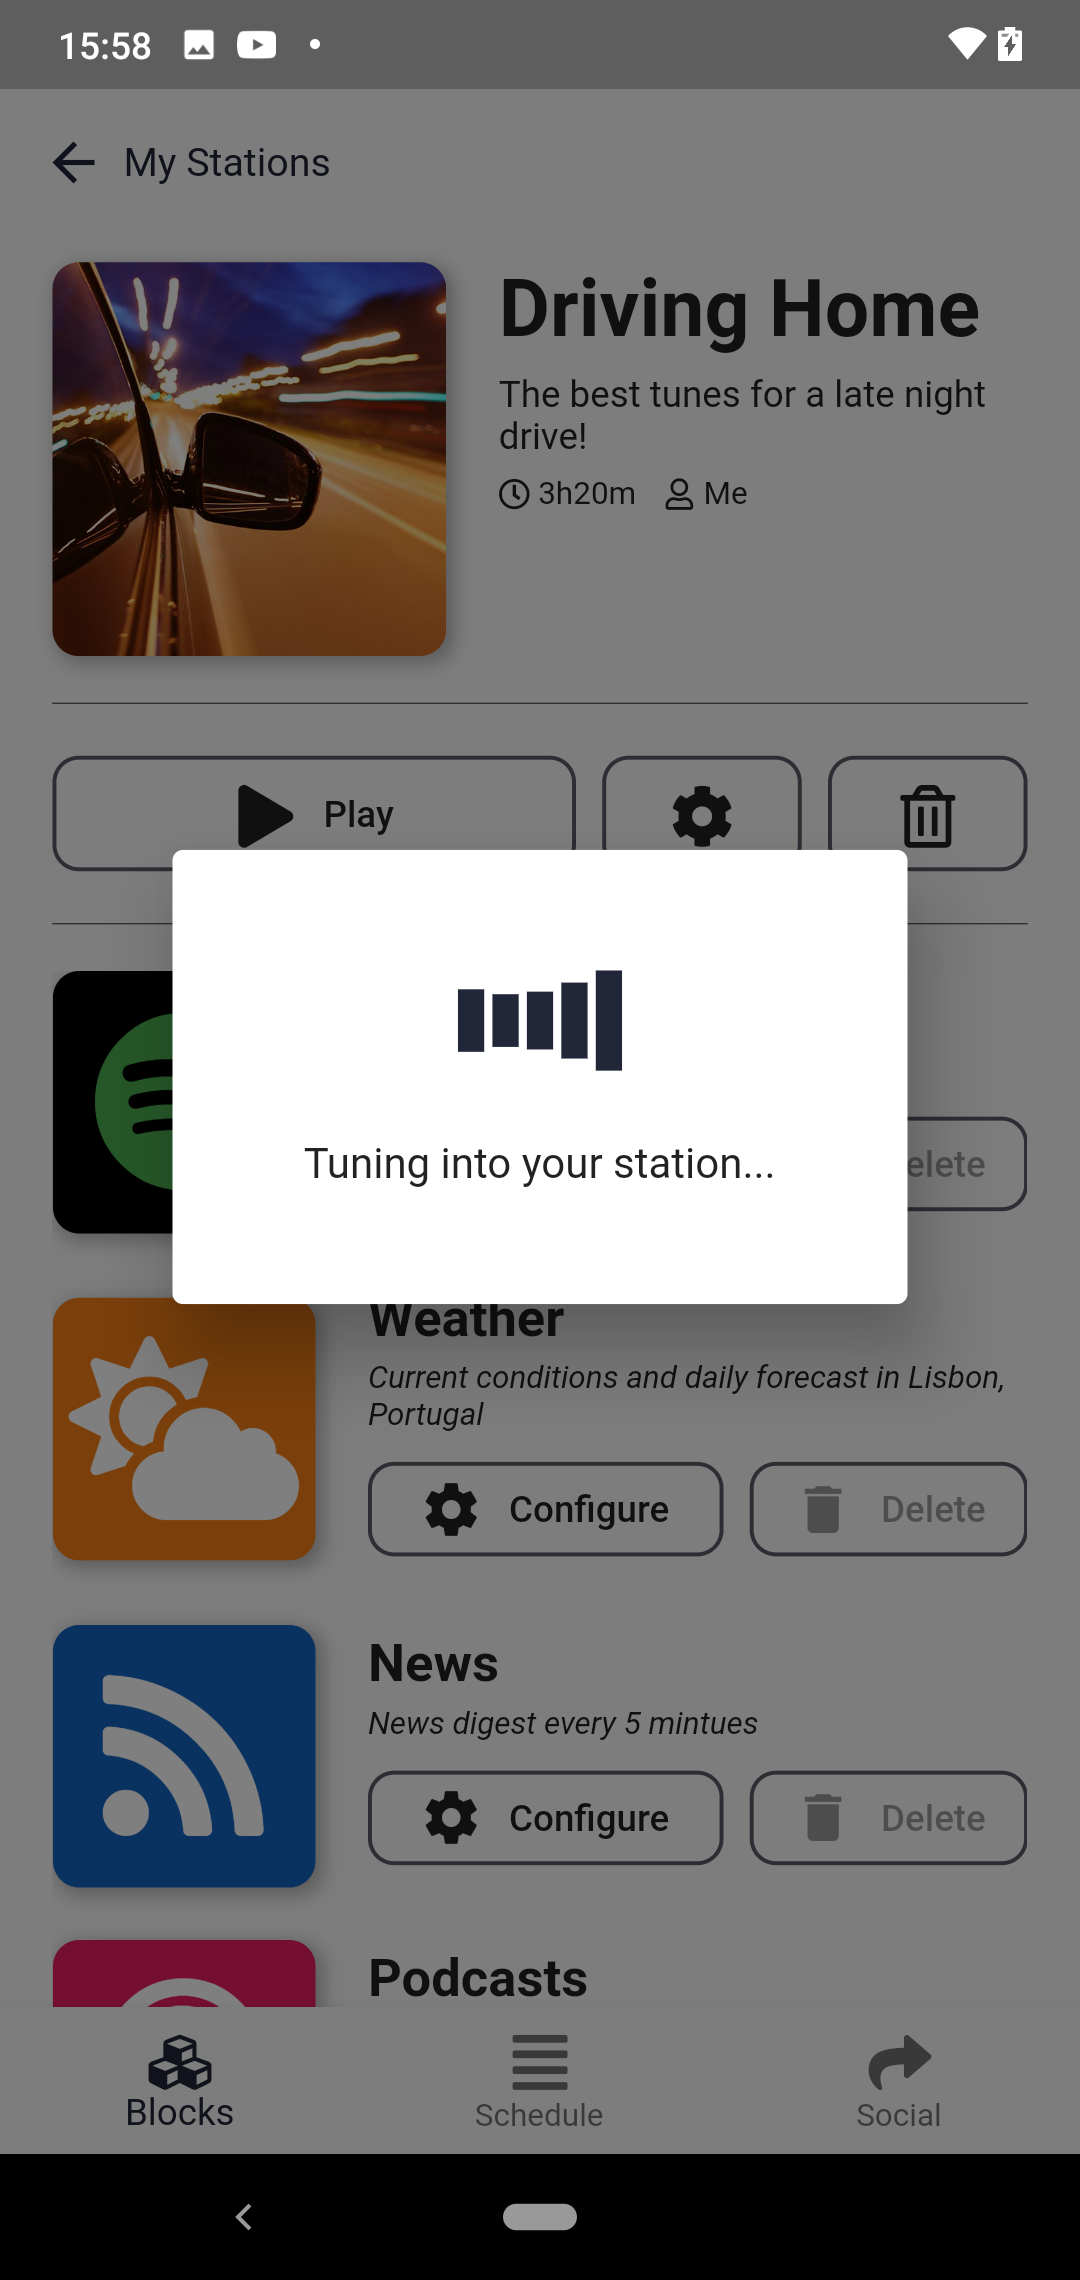
\includegraphics[width=0.29\textwidth]{./Images/screenshots/play1.png}}} \qquad
	\subfigure["Now Playing" controller bottom bar]{\label{fig:play2}
	\frame{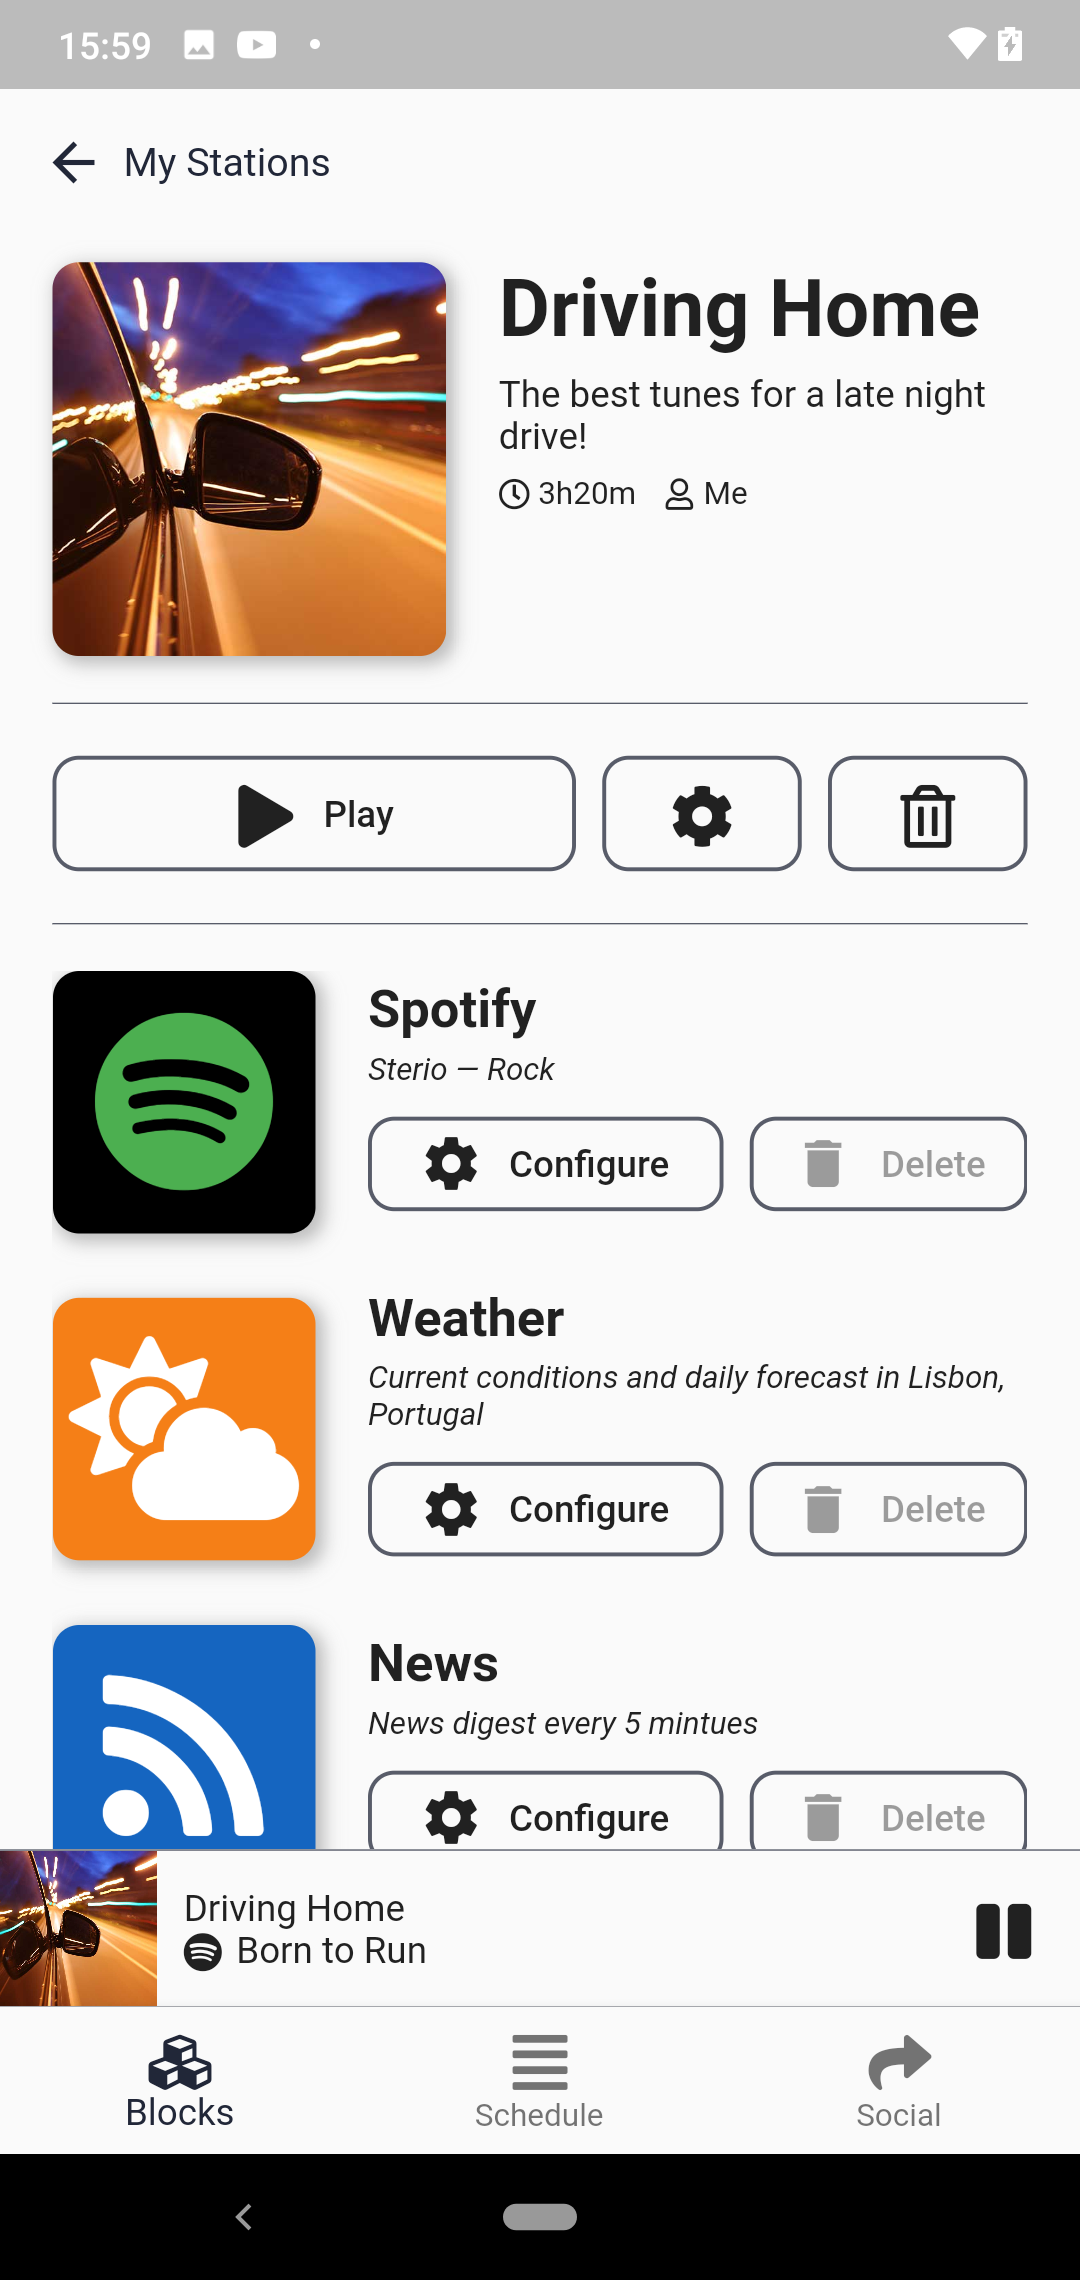
\includegraphics[width=0.29\textwidth]{./Images/screenshots/play2.png}}} \qquad
	\caption{Playing a station}
	\label{fig:mfp1}
\end{figure}

\newpage

Finally, the station starts playing, and a 'Now Playing' controller bar, shown in Figure ~\ref{fig:play2}, is displayed. This bar provides quick and easy information to the user regarding what's currently playing, as well as a 'Play/Pause' button to stop playback when needed. If the user taps this bar, the 'Now Playing' screen, showcased in Figure ~\ref{fig:npslol} is shown, which provides more playback controls and information regarding the currently playing station, including the content that will be played next in the schedule.

\begin{figure}[htbp]
	\centering
	\subfigure[Now playing screen]{\label{fig:np1}
	\frame{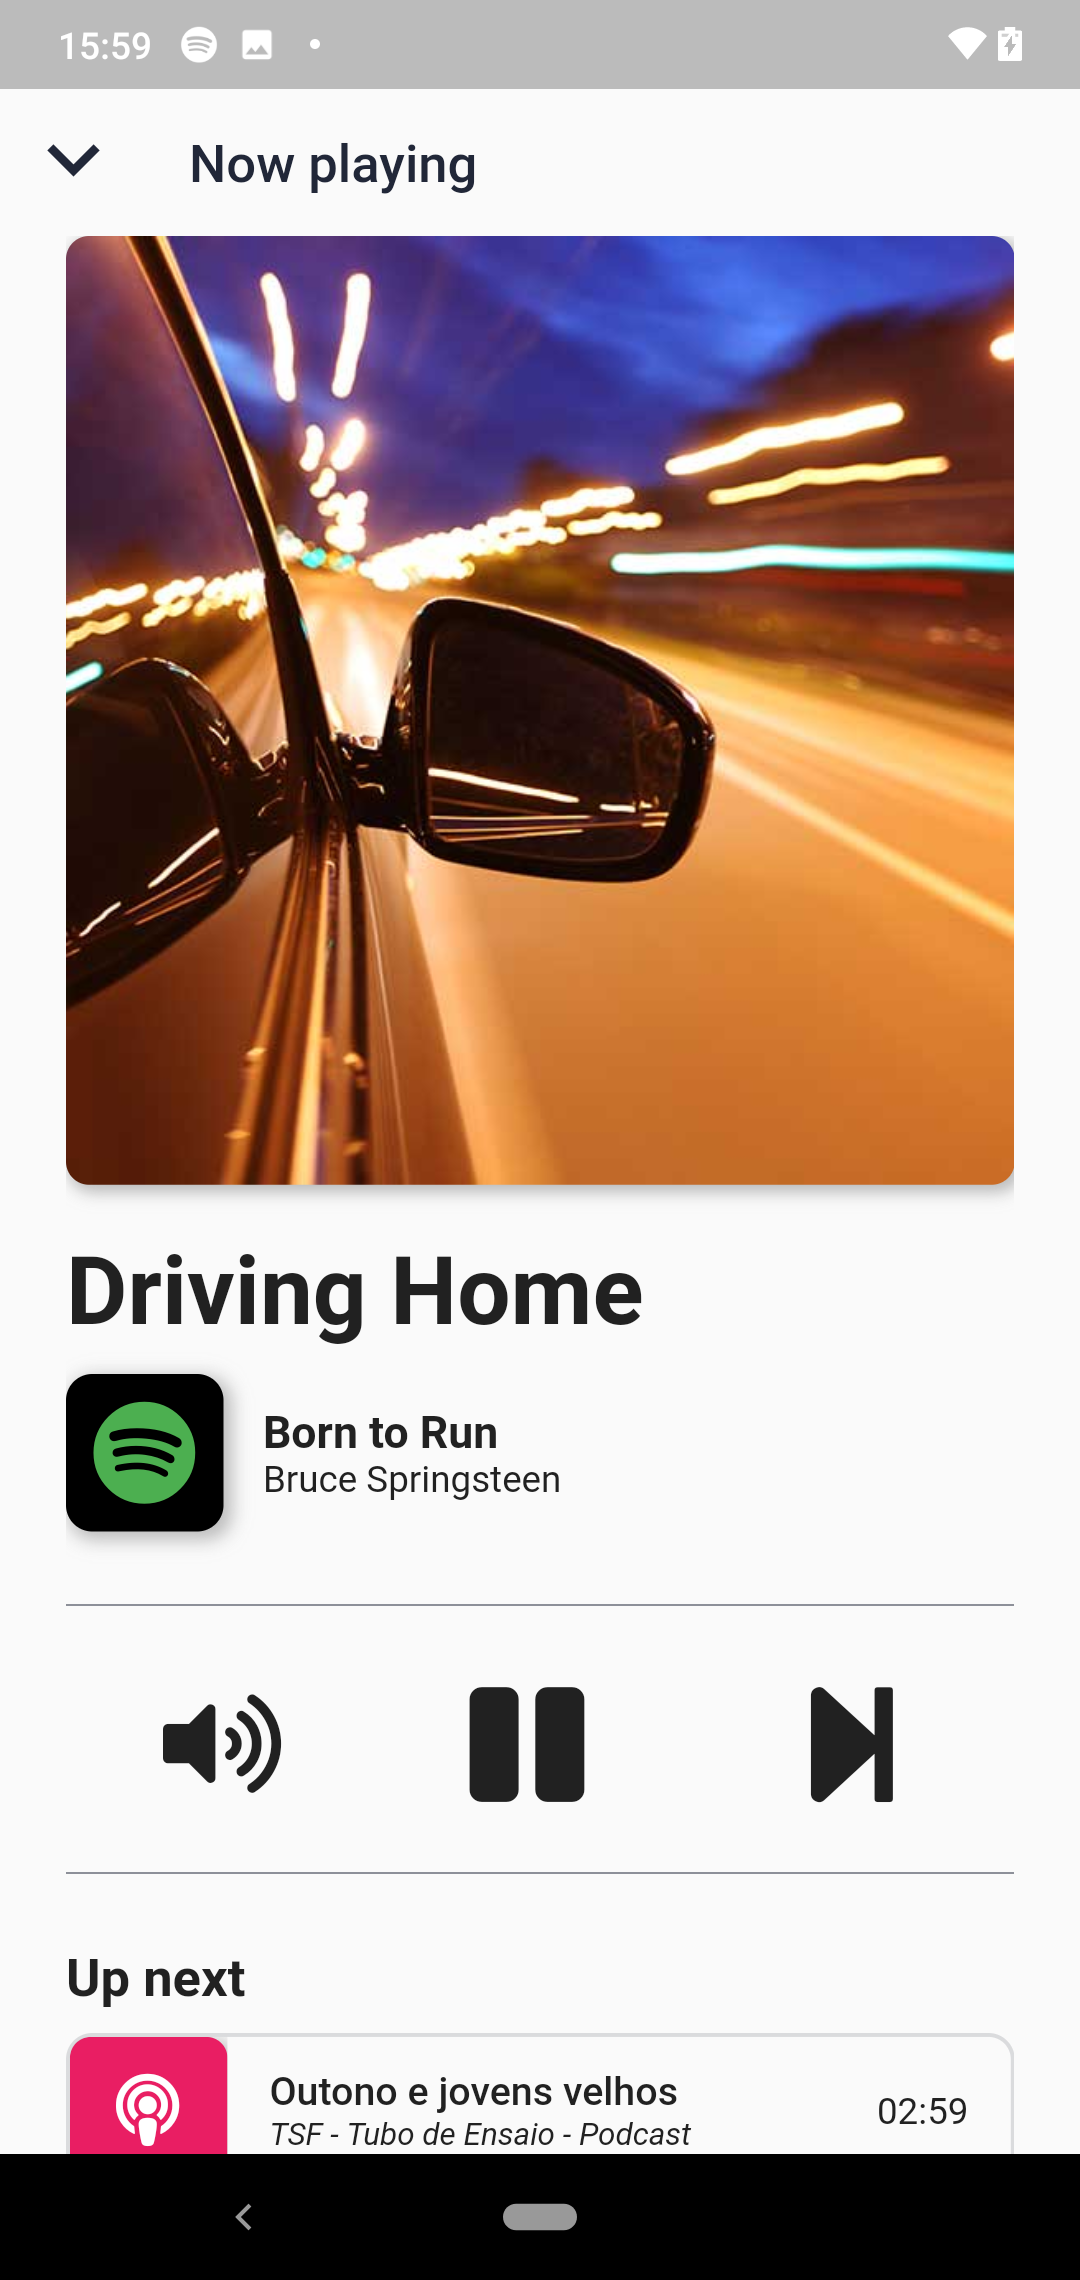
\includegraphics[width=0.29\textwidth]{./Images/screenshots/np1.png}}} \qquad
	\subfigure[Up next content]{\label{fig:np2}
	\frame{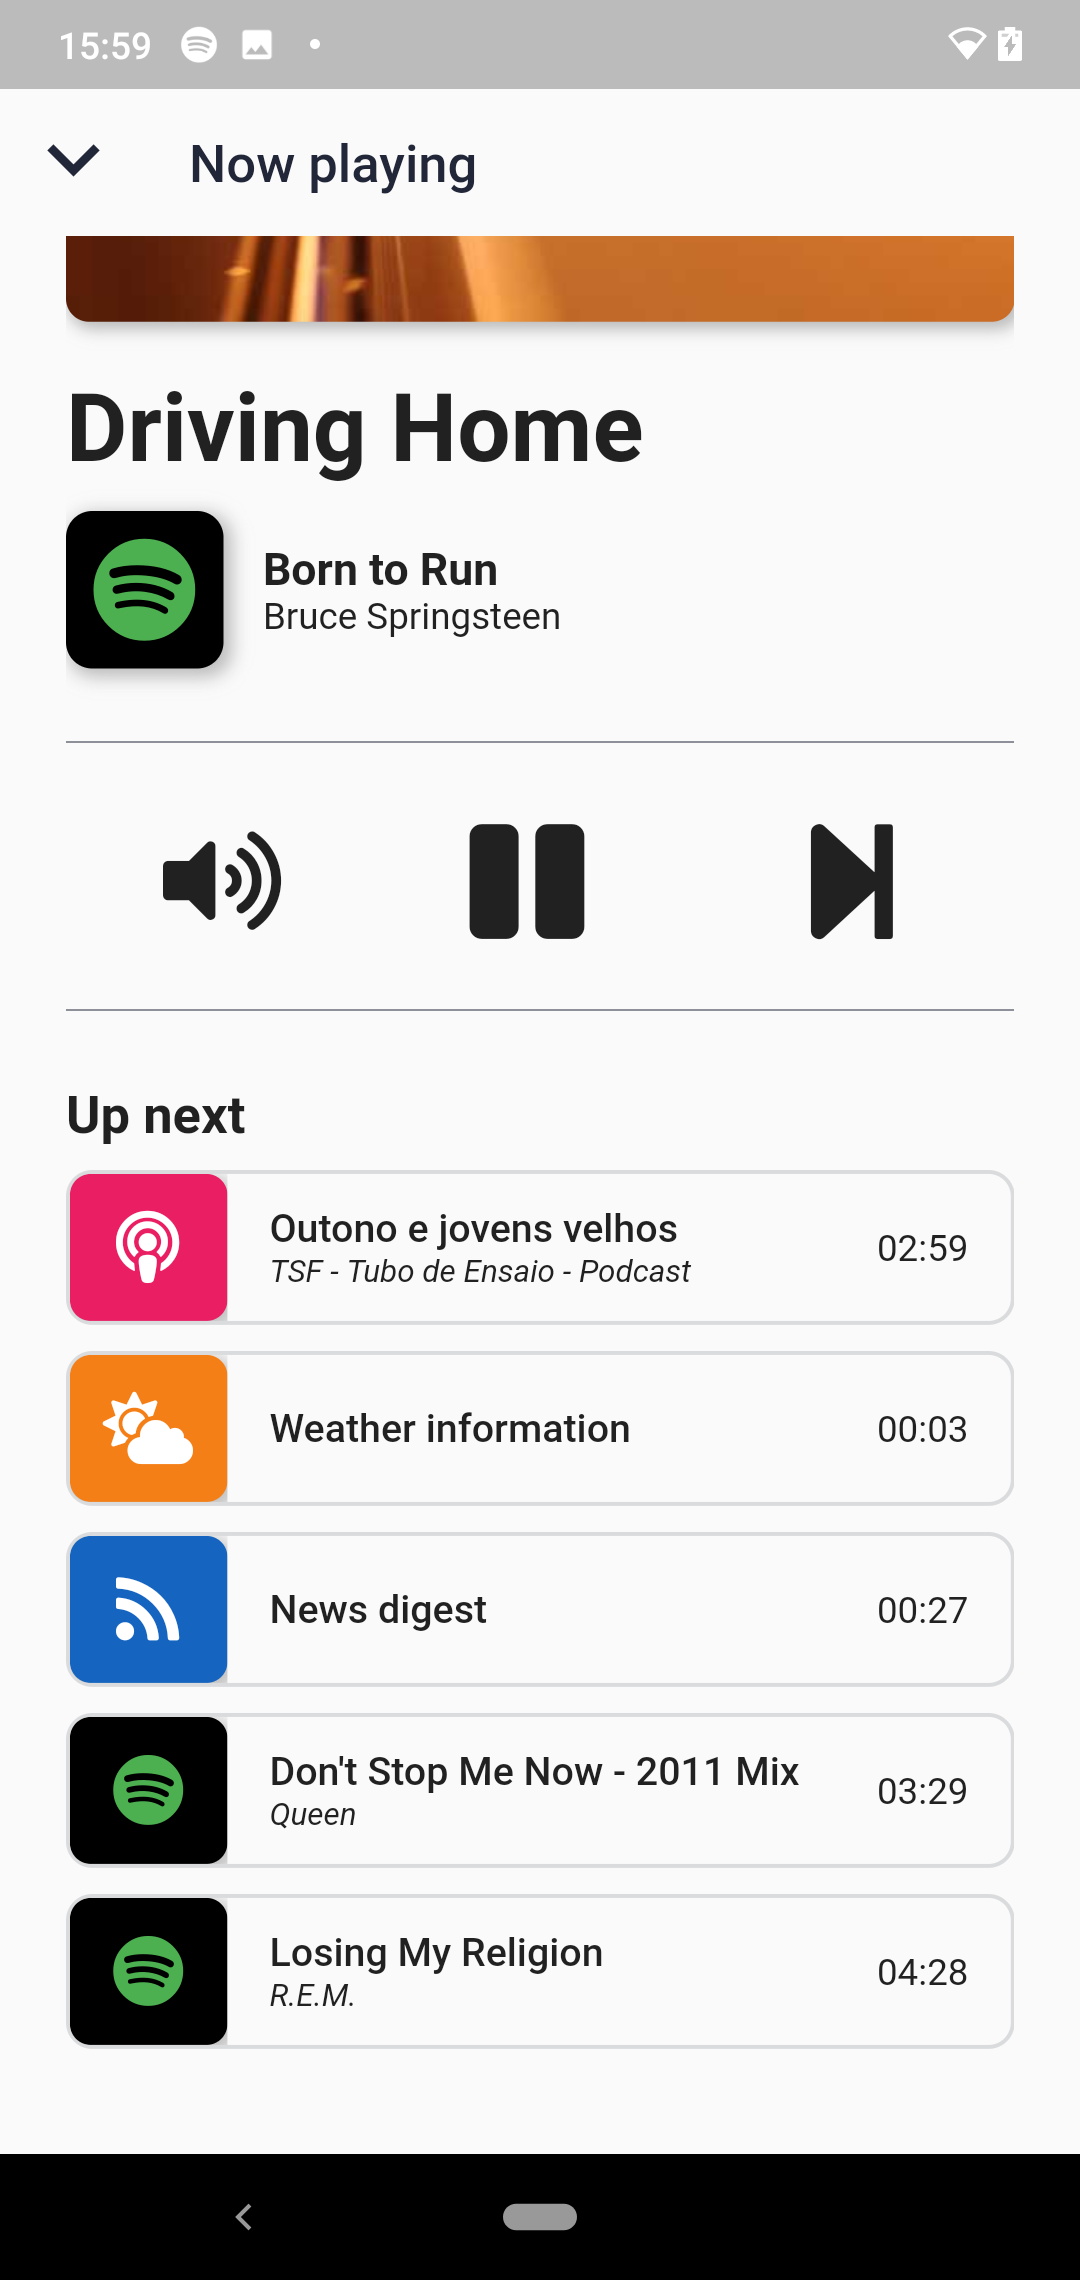
\includegraphics[width=0.29\textwidth]{./Images/screenshots/np2.png}}} \qquad
	\caption{"Now Playing" screen}
	\label{fig:npslol}
\end{figure}

\begin{figure}[h]
\centering
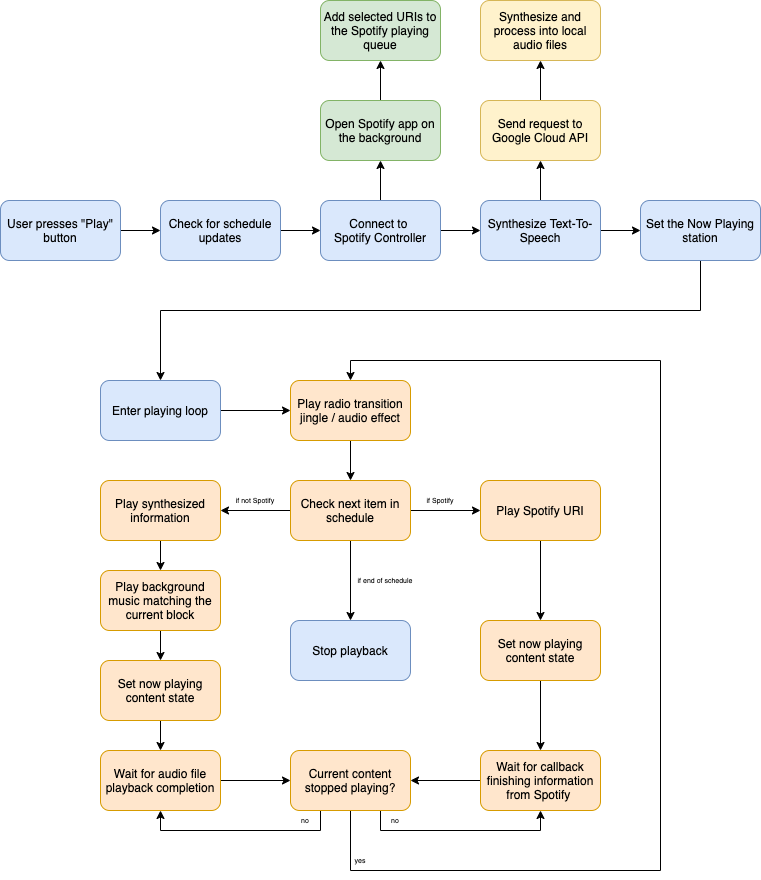
\includegraphics[width=0.8\textwidth]{./Images/code/alg.png}
\caption{Algorithm for playing a given station}
\label{fig:alg}
\end{figure}


To play the station, a 5-step algorithm is performed before entering the main playing loop. This algorithm is represented in Figure ~\ref{fig:alg}.

After pressing the play button, the first step of the algorithm is to check if the user has changed the configurations of any of the selected blocks, or if the schedule playing order has been modified. If it is the case, the algorithm updates and processes the schedule so that it is performed on the most recent configurations of the station.

Following this process, the platform will connect to the Spotify Controller, which is a dedicated component of the code that connects to the Spotify Playback \ac{API}. As mentioned in Section ~\ref{sub:spotify}, this is a different \ac{API} library from the one used to select the desired content from the music streaming service.

To control a user's Spotify playback, the \ac{API} requires that the Spotify application is installed on the user's device and that it is opened in the background, so that it can receive requests. This is a limitation set by the Spotify \ac{API} that we can't bypass. After the connection to the Spotify Controller is successful, then all the selected content (\acp{URI}) is added to the user's Spotify listening queue.

After the Spotify connection is handled, all the information from the remaining station's blocks is fetched, so that it is as updated and real-time as possible. The responses are then processed into a natural spoken text, which is then sent as a 'GET' request to the Google Cloud Text-to-Speech API~\footnote{For more information on used API for the text-to-speech synthesizer, visit the \href{https://cloud.google.com/text-to-speech/docs}{Google Cloud Text-to-Speech API website.}}. The API responds with a set of encoded information containing the synthesized sound bytes, which are locally converted into audio files. These audio files are then stored in the cache of the platform which, after playing the station, are discarded to save storage space.

Then, if Spotify successfully connected to the platform, and if all the requested information from the blocks is successfully synthesized into text-to-speech audio files, the last step before entering the main playing loop is to set the 'Now Playing' station as the current 'state' of the platform. This allows the access and control of the currently playing station throughout the interface, as shown in Figures ~\ref{fig:play2} and ~\ref{fig:npslol}.

Finally, the station enters its main playing loop. Every station begins with a radio transition jingle or audio effect that serves as a separator between content, mimicking a traditional terrestrial radio station, and granting a more cohesive and integrated experience to the user. This transition is naturally inserted between music tracks or other content to allow continued attention in the periphery. Transitions can also be turned off if the user wants a more synthetic listening experience.

Following this introductory audio effect, the algorithm checks whether the next item of the schedule is a Spotify \ac{URI} or not. If it is, it plays it by simply calling a 'play' function provided by the Spotify Controller, and sets the now playing state of the application. Then, the algorithm checks if the current Spotify content has finished playing, and, if so, it plays an audio transition and another iteration of the loop is processed.

The most difficult challenge we faced while coding this algorithm was the process of determining whether the Spotify content has finished playing or not. The Spotify Playback \ac{API} does not provide an easy way of accessing this information, allowing only the access of a limited set of playback information, such as the current position of a content's playback. To bypass this limitation, we crafted a sub-algorithm that checks second by second this information, and when the current position of a content's playback matches the total length of such content, an alert is sent to indicate that the content has finished playing. This approach adds complexity in terms of performance and resource usage, but it was the only way we found to bypass this limitation set by the Spotify Playback \ac{API}.

Conversely, if the next item on the schedule is not a Spotify \ac{URI}, then the algorithm picks up the matching synthesized audio file and plays it. At the same time, matching background music is added while the text-to-speech audio file is played, so that the user creates more empathy while listening to the information. The now playing state of the application is also set, and if the algorithm checks if the current content has finished playing, it plays an audio transition, and another iteration of the loop is processed. As we're processing local files, we didn't face the same issues in determining if the currently playing content has finished playing, unlike we had with Spotify content playback.

When the station finishes playing its matching schedule, the playback is stopped and all the local cached files are deleted. Nevertheless, the user can choose to loop or repeat the station, allowing a non-stop playback of content.

